\documentclass[twoside]{book}

% Packages required by doxygen
\usepackage{calc}
\usepackage{doxygen}
\usepackage{graphicx}
\usepackage[utf8]{inputenc}
\usepackage{makeidx}
\usepackage{multicol}
\usepackage{multirow}
\usepackage{textcomp}
\usepackage[table]{xcolor}

% Font selection
\usepackage[T1]{fontenc}
\usepackage{mathptmx}
\usepackage[scaled=.90]{helvet}
\usepackage{courier}
\usepackage{amssymb}
\usepackage{sectsty}
\renewcommand{\familydefault}{\sfdefault}
\allsectionsfont{%
  \fontseries{bc}\selectfont%
  \color{darkgray}%
}
\renewcommand{\DoxyLabelFont}{%
  \fontseries{bc}\selectfont%
  \color{darkgray}%
}

% Page & text layout
\usepackage{geometry}
\geometry{%
  a4paper,%
  top=2.5cm,%
  bottom=2.5cm,%
  left=2.5cm,%
  right=2.5cm%
}
\tolerance=750
\hfuzz=15pt
\hbadness=750
\setlength{\emergencystretch}{15pt}
\setlength{\parindent}{0cm}
\setlength{\parskip}{0.2cm}
\makeatletter
\renewcommand{\paragraph}{%
  \@startsection{paragraph}{4}{0ex}{-1.0ex}{1.0ex}{%
    \normalfont\normalsize\bfseries\SS@parafont%
  }%
}
\renewcommand{\subparagraph}{%
  \@startsection{subparagraph}{5}{0ex}{-1.0ex}{1.0ex}{%
    \normalfont\normalsize\bfseries\SS@subparafont%
  }%
}
\makeatother

% Headers & footers
\usepackage{fancyhdr}
\pagestyle{fancyplain}
\fancyhead[LE]{\fancyplain{}{\bfseries\thepage}}
\fancyhead[CE]{\fancyplain{}{}}
\fancyhead[RE]{\fancyplain{}{\bfseries\leftmark}}
\fancyhead[LO]{\fancyplain{}{\bfseries\rightmark}}
\fancyhead[CO]{\fancyplain{}{}}
\fancyhead[RO]{\fancyplain{}{\bfseries\thepage}}
\fancyfoot[LE]{\fancyplain{}{}}
\fancyfoot[CE]{\fancyplain{}{}}
\fancyfoot[RE]{\fancyplain{}{\bfseries\scriptsize Generated on Wed Dec 4 2013 09\-:49\-:08 for Workout App by Doxygen }}
\fancyfoot[LO]{\fancyplain{}{\bfseries\scriptsize Generated on Wed Dec 4 2013 09\-:49\-:08 for Workout App by Doxygen }}
\fancyfoot[CO]{\fancyplain{}{}}
\fancyfoot[RO]{\fancyplain{}{}}
\renewcommand{\footrulewidth}{0.4pt}
\renewcommand{\chaptermark}[1]{%
  \markboth{#1}{}%
}
\renewcommand{\sectionmark}[1]{%
  \markright{\thesection\ #1}%
}

% Indices & bibliography
\usepackage{natbib}
\usepackage[titles]{tocloft}
\setcounter{tocdepth}{3}
\setcounter{secnumdepth}{5}
\makeindex

% Hyperlinks (required, but should be loaded last)
\usepackage{ifpdf}
\ifpdf
  \usepackage[pdftex,pagebackref=true]{hyperref}
\else
  \usepackage[ps2pdf,pagebackref=true]{hyperref}
\fi
\hypersetup{%
  colorlinks=true,%
  linkcolor=blue,%
  citecolor=blue,%
  unicode%
}

% Custom commands
\newcommand{\clearemptydoublepage}{%
  \newpage{\pagestyle{empty}\cleardoublepage}%
}


%===== C O N T E N T S =====

\begin{document}

% Titlepage & ToC
\hypersetup{pageanchor=false}
\pagenumbering{roman}
\begin{titlepage}
\vspace*{7cm}
\begin{center}%
{\Large Workout App }\\
\vspace*{1cm}
{\large Generated by Doxygen 1.8.5}\\
\vspace*{0.5cm}
{\small Wed Dec 4 2013 09:49:08}\\
\end{center}
\end{titlepage}
\clearemptydoublepage
\tableofcontents
\clearemptydoublepage
\pagenumbering{arabic}
\hypersetup{pageanchor=true}

%--- Begin generated contents ---
\chapter{Namespace Index}
\section{Packages}
Here are the packages with brief descriptions (if available)\-:\begin{DoxyCompactList}
\item\contentsline{section}{\hyperlink{namespacecom}{com} }{\pageref{namespacecom}}{}
\item\contentsline{section}{\hyperlink{namespacecom_1_1example}{com.\-example} }{\pageref{namespacecom_1_1example}}{}
\item\contentsline{section}{\hyperlink{namespacecom_1_1example_1_1workoutcompanion}{com.\-example.\-workoutcompanion} }{\pageref{namespacecom_1_1example_1_1workoutcompanion}}{}
\item\contentsline{section}{\hyperlink{namespacecom_1_1example_1_1workoutcompanion_1_1controller}{com.\-example.\-workoutcompanion.\-controller} }{\pageref{namespacecom_1_1example_1_1workoutcompanion_1_1controller}}{}
\item\contentsline{section}{\hyperlink{namespacecom_1_1example_1_1workoutcompanion_1_1db}{com.\-example.\-workoutcompanion.\-db} }{\pageref{namespacecom_1_1example_1_1workoutcompanion_1_1db}}{}
\item\contentsline{section}{\hyperlink{namespacecom_1_1example_1_1workoutcompanion_1_1dom}{com.\-example.\-workoutcompanion.\-dom} }{\pageref{namespacecom_1_1example_1_1workoutcompanion_1_1dom}}{}
\end{DoxyCompactList}

\chapter{Hierarchical Index}
\section{Class Hierarchy}
This inheritance list is sorted roughly, but not completely, alphabetically\-:\begin{DoxyCompactList}
\item \contentsline{section}{com.\-example.\-workoutcompanion.\-Build\-Config}{\pageref{classcom_1_1example_1_1workoutcompanion_1_1_build_config}}{}
\item \contentsline{section}{com.\-example.\-workoutcompanion.\-controller.\-Command}{\pageref{interfacecom_1_1example_1_1workoutcompanion_1_1controller_1_1_command}}{}
\begin{DoxyCompactList}
\item \contentsline{section}{com.\-example.\-workoutcompanion.\-controller.\-Create\-Exercise\-Cmd}{\pageref{classcom_1_1example_1_1workoutcompanion_1_1controller_1_1_create_exercise_cmd}}{}
\item \contentsline{section}{com.\-example.\-workoutcompanion.\-controller.\-Create\-Workout\-Cmd}{\pageref{classcom_1_1example_1_1workoutcompanion_1_1controller_1_1_create_workout_cmd}}{}
\item \contentsline{section}{com.\-example.\-workoutcompanion.\-controller.\-Edit\-Exercise\-Cmd}{\pageref{classcom_1_1example_1_1workoutcompanion_1_1controller_1_1_edit_exercise_cmd}}{}
\item \contentsline{section}{com.\-example.\-workoutcompanion.\-controller.\-Edit\-Profile\-Cmd}{\pageref{classcom_1_1example_1_1workoutcompanion_1_1controller_1_1_edit_profile_cmd}}{}
\item \contentsline{section}{com.\-example.\-workoutcompanion.\-controller.\-Edit\-Workout\-Cmd}{\pageref{classcom_1_1example_1_1workoutcompanion_1_1controller_1_1_edit_workout_cmd}}{}
\begin{DoxyCompactList}
\item \contentsline{section}{com.\-example.\-workoutcompanion.\-controller.\-Add\-Exercise\-To\-Workout\-Cmd}{\pageref{classcom_1_1example_1_1workoutcompanion_1_1controller_1_1_add_exercise_to_workout_cmd}}{}
\item \contentsline{section}{com.\-example.\-workoutcompanion.\-controller.\-Remove\-Exercise\-From\-Workout\-Cmd}{\pageref{classcom_1_1example_1_1workoutcompanion_1_1controller_1_1_remove_exercise_from_workout_cmd}}{}
\end{DoxyCompactList}
\end{DoxyCompactList}
\item \contentsline{section}{com.\-example.\-workoutcompanion.\-controller.\-Controller}{\pageref{classcom_1_1example_1_1workoutcompanion_1_1controller_1_1_controller}}{}
\item \contentsline{section}{com.\-example.\-workoutcompanion.\-dom.\-Exercise}{\pageref{classcom_1_1example_1_1workoutcompanion_1_1dom_1_1_exercise}}{}
\item \contentsline{section}{com.\-example.\-workoutcompanion.\-dom.\-Profile}{\pageref{classcom_1_1example_1_1workoutcompanion_1_1dom_1_1_profile}}{}
\item \contentsline{section}{com.\-example.\-workoutcompanion.\-R}{\pageref{classcom_1_1example_1_1workoutcompanion_1_1_r}}{}
\item \contentsline{section}{com.\-example.\-workoutcompanion.\-controller.\-Receiver}{\pageref{classcom_1_1example_1_1workoutcompanion_1_1controller_1_1_receiver}}{}
\item \contentsline{section}{com.\-example.\-workoutcompanion.\-dom.\-Table\-Record}{\pageref{classcom_1_1example_1_1workoutcompanion_1_1dom_1_1_table_record}}{}
\begin{DoxyCompactList}
\item \contentsline{section}{com.\-example.\-workoutcompanion.\-dom.\-Workout\-Component}{\pageref{classcom_1_1example_1_1workoutcompanion_1_1dom_1_1_workout_component}}{}
\end{DoxyCompactList}
\item Tab\-Listener\begin{DoxyCompactList}
\item \contentsline{section}{com.\-example.\-workoutcompanion.\-Workout\-Activity}{\pageref{classcom_1_1example_1_1workoutcompanion_1_1_workout_activity}}{}
\end{DoxyCompactList}
\item \contentsline{section}{com.\-example.\-workoutcompanion.\-dom.\-Workout}{\pageref{classcom_1_1example_1_1workoutcompanion_1_1dom_1_1_workout}}{}
\item Activity\begin{DoxyCompactList}
\item \contentsline{section}{com.\-example.\-workoutcompanion.\-Edit\-Activity}{\pageref{classcom_1_1example_1_1workoutcompanion_1_1_edit_activity}}{}
\end{DoxyCompactList}
\item Base\-Expandable\-List\-Adapter\begin{DoxyCompactList}
\item \contentsline{section}{com.\-example.\-workoutcompanion.\-Workout\-List\-Adapter}{\pageref{classcom_1_1example_1_1workoutcompanion_1_1_workout_list_adapter}}{}
\end{DoxyCompactList}
\item Fragment\begin{DoxyCompactList}
\item \contentsline{section}{com.\-example.\-workoutcompanion.\-Profile\-Fragment}{\pageref{classcom_1_1example_1_1workoutcompanion_1_1_profile_fragment}}{}
\item \contentsline{section}{com.\-example.\-workoutcompanion.\-Workout\-Fragment}{\pageref{classcom_1_1example_1_1workoutcompanion_1_1_workout_fragment}}{}
\end{DoxyCompactList}
\item Fragment\-Activity\begin{DoxyCompactList}
\item \contentsline{section}{com.\-example.\-workoutcompanion.\-Workout\-Activity}{\pageref{classcom_1_1example_1_1workoutcompanion_1_1_workout_activity}}{}
\end{DoxyCompactList}
\item Fragment\-Pager\-Adapter\begin{DoxyCompactList}
\item \contentsline{section}{com.\-example.\-workoutcompanion.\-Sections\-Pager\-Adapter}{\pageref{classcom_1_1example_1_1workoutcompanion_1_1_sections_pager_adapter}}{}
\end{DoxyCompactList}
\item List\-Activity\begin{DoxyCompactList}
\item \contentsline{section}{com.\-example.\-workoutcompanion.\-Add\-Exercise\-Activity}{\pageref{classcom_1_1example_1_1workoutcompanion_1_1_add_exercise_activity}}{}
\end{DoxyCompactList}
\item Orm\-Lite\-Sqlite\-Open\-Helper\begin{DoxyCompactList}
\item \contentsline{section}{com.\-example.\-workoutcompanion.\-db.\-Database\-Handler}{\pageref{classcom_1_1example_1_1workoutcompanion_1_1db_1_1_database_handler}}{}
\end{DoxyCompactList}
\end{DoxyCompactList}

\chapter{Class Index}
\section{Class List}
Here are the classes, structs, unions and interfaces with brief descriptions\-:\begin{DoxyCompactList}
\item\contentsline{section}{\hyperlink{classcom_1_1example_1_1workoutcompanion_1_1_add_exercise_activity}{com.\-example.\-workoutcompanion.\-Add\-Exercise\-Activity} }{\pageref{classcom_1_1example_1_1workoutcompanion_1_1_add_exercise_activity}}{}
\item\contentsline{section}{\hyperlink{classcom_1_1example_1_1workoutcompanion_1_1controller_1_1_add_exercise_to_workout_cmd}{com.\-example.\-workoutcompanion.\-controller.\-Add\-Exercise\-To\-Workout\-Cmd} }{\pageref{classcom_1_1example_1_1workoutcompanion_1_1controller_1_1_add_exercise_to_workout_cmd}}{}
\item\contentsline{section}{\hyperlink{classcom_1_1example_1_1workoutcompanion_1_1_build_config}{com.\-example.\-workoutcompanion.\-Build\-Config} }{\pageref{classcom_1_1example_1_1workoutcompanion_1_1_build_config}}{}
\item\contentsline{section}{\hyperlink{interfacecom_1_1example_1_1workoutcompanion_1_1controller_1_1_command}{com.\-example.\-workoutcompanion.\-controller.\-Command} }{\pageref{interfacecom_1_1example_1_1workoutcompanion_1_1controller_1_1_command}}{}
\item\contentsline{section}{\hyperlink{classcom_1_1example_1_1workoutcompanion_1_1controller_1_1_controller}{com.\-example.\-workoutcompanion.\-controller.\-Controller} }{\pageref{classcom_1_1example_1_1workoutcompanion_1_1controller_1_1_controller}}{}
\item\contentsline{section}{\hyperlink{classcom_1_1example_1_1workoutcompanion_1_1controller_1_1_create_exercise_cmd}{com.\-example.\-workoutcompanion.\-controller.\-Create\-Exercise\-Cmd} }{\pageref{classcom_1_1example_1_1workoutcompanion_1_1controller_1_1_create_exercise_cmd}}{}
\item\contentsline{section}{\hyperlink{classcom_1_1example_1_1workoutcompanion_1_1controller_1_1_create_workout_cmd}{com.\-example.\-workoutcompanion.\-controller.\-Create\-Workout\-Cmd} }{\pageref{classcom_1_1example_1_1workoutcompanion_1_1controller_1_1_create_workout_cmd}}{}
\item\contentsline{section}{\hyperlink{classcom_1_1example_1_1workoutcompanion_1_1db_1_1_database_handler}{com.\-example.\-workoutcompanion.\-db.\-Database\-Handler} }{\pageref{classcom_1_1example_1_1workoutcompanion_1_1db_1_1_database_handler}}{}
\item\contentsline{section}{\hyperlink{classcom_1_1example_1_1workoutcompanion_1_1_edit_activity}{com.\-example.\-workoutcompanion.\-Edit\-Activity} }{\pageref{classcom_1_1example_1_1workoutcompanion_1_1_edit_activity}}{}
\item\contentsline{section}{\hyperlink{classcom_1_1example_1_1workoutcompanion_1_1controller_1_1_edit_exercise_cmd}{com.\-example.\-workoutcompanion.\-controller.\-Edit\-Exercise\-Cmd} }{\pageref{classcom_1_1example_1_1workoutcompanion_1_1controller_1_1_edit_exercise_cmd}}{}
\item\contentsline{section}{\hyperlink{classcom_1_1example_1_1workoutcompanion_1_1controller_1_1_edit_profile_cmd}{com.\-example.\-workoutcompanion.\-controller.\-Edit\-Profile\-Cmd} }{\pageref{classcom_1_1example_1_1workoutcompanion_1_1controller_1_1_edit_profile_cmd}}{}
\item\contentsline{section}{\hyperlink{classcom_1_1example_1_1workoutcompanion_1_1controller_1_1_edit_workout_cmd}{com.\-example.\-workoutcompanion.\-controller.\-Edit\-Workout\-Cmd} }{\pageref{classcom_1_1example_1_1workoutcompanion_1_1controller_1_1_edit_workout_cmd}}{}
\item\contentsline{section}{\hyperlink{classcom_1_1example_1_1workoutcompanion_1_1dom_1_1_exercise}{com.\-example.\-workoutcompanion.\-dom.\-Exercise} }{\pageref{classcom_1_1example_1_1workoutcompanion_1_1dom_1_1_exercise}}{}
\item\contentsline{section}{\hyperlink{classcom_1_1example_1_1workoutcompanion_1_1dom_1_1_profile}{com.\-example.\-workoutcompanion.\-dom.\-Profile} }{\pageref{classcom_1_1example_1_1workoutcompanion_1_1dom_1_1_profile}}{}
\item\contentsline{section}{\hyperlink{classcom_1_1example_1_1workoutcompanion_1_1_profile_fragment}{com.\-example.\-workoutcompanion.\-Profile\-Fragment} }{\pageref{classcom_1_1example_1_1workoutcompanion_1_1_profile_fragment}}{}
\item\contentsline{section}{\hyperlink{classcom_1_1example_1_1workoutcompanion_1_1_r}{com.\-example.\-workoutcompanion.\-R} }{\pageref{classcom_1_1example_1_1workoutcompanion_1_1_r}}{}
\item\contentsline{section}{\hyperlink{classcom_1_1example_1_1workoutcompanion_1_1controller_1_1_receiver}{com.\-example.\-workoutcompanion.\-controller.\-Receiver} }{\pageref{classcom_1_1example_1_1workoutcompanion_1_1controller_1_1_receiver}}{}
\item\contentsline{section}{\hyperlink{classcom_1_1example_1_1workoutcompanion_1_1controller_1_1_remove_exercise_from_workout_cmd}{com.\-example.\-workoutcompanion.\-controller.\-Remove\-Exercise\-From\-Workout\-Cmd} }{\pageref{classcom_1_1example_1_1workoutcompanion_1_1controller_1_1_remove_exercise_from_workout_cmd}}{}
\item\contentsline{section}{\hyperlink{classcom_1_1example_1_1workoutcompanion_1_1_sections_pager_adapter}{com.\-example.\-workoutcompanion.\-Sections\-Pager\-Adapter} }{\pageref{classcom_1_1example_1_1workoutcompanion_1_1_sections_pager_adapter}}{}
\item\contentsline{section}{\hyperlink{classcom_1_1example_1_1workoutcompanion_1_1dom_1_1_table_record}{com.\-example.\-workoutcompanion.\-dom.\-Table\-Record} }{\pageref{classcom_1_1example_1_1workoutcompanion_1_1dom_1_1_table_record}}{}
\item\contentsline{section}{\hyperlink{classcom_1_1example_1_1workoutcompanion_1_1dom_1_1_workout}{com.\-example.\-workoutcompanion.\-dom.\-Workout} }{\pageref{classcom_1_1example_1_1workoutcompanion_1_1dom_1_1_workout}}{}
\item\contentsline{section}{\hyperlink{classcom_1_1example_1_1workoutcompanion_1_1_workout_activity}{com.\-example.\-workoutcompanion.\-Workout\-Activity} }{\pageref{classcom_1_1example_1_1workoutcompanion_1_1_workout_activity}}{}
\item\contentsline{section}{\hyperlink{classcom_1_1example_1_1workoutcompanion_1_1dom_1_1_workout_component}{com.\-example.\-workoutcompanion.\-dom.\-Workout\-Component} }{\pageref{classcom_1_1example_1_1workoutcompanion_1_1dom_1_1_workout_component}}{}
\item\contentsline{section}{\hyperlink{classcom_1_1example_1_1workoutcompanion_1_1_workout_fragment}{com.\-example.\-workoutcompanion.\-Workout\-Fragment} }{\pageref{classcom_1_1example_1_1workoutcompanion_1_1_workout_fragment}}{}
\item\contentsline{section}{\hyperlink{classcom_1_1example_1_1workoutcompanion_1_1_workout_list_adapter}{com.\-example.\-workoutcompanion.\-Workout\-List\-Adapter} }{\pageref{classcom_1_1example_1_1workoutcompanion_1_1_workout_list_adapter}}{}
\end{DoxyCompactList}

\chapter{File Index}
\section{File List}
Here is a list of all files with brief descriptions\-:\begin{DoxyCompactList}
\item\contentsline{section}{Desktop/git\-\_\-proj/workout/gen/com/example/workoutcompanion/\hyperlink{_build_config_8java}{Build\-Config.\-java} }{\pageref{_build_config_8java}}{}
\item\contentsline{section}{Desktop/git\-\_\-proj/workout/gen/com/example/workoutcompanion/\hyperlink{_r_8java}{R.\-java} }{\pageref{_r_8java}}{}
\item\contentsline{section}{Desktop/git\-\_\-proj/workout/src/com/example/workoutcompanion/\hyperlink{_add_exercise_activity_8java}{Add\-Exercise\-Activity.\-java} }{\pageref{_add_exercise_activity_8java}}{}
\item\contentsline{section}{Desktop/git\-\_\-proj/workout/src/com/example/workoutcompanion/\hyperlink{_edit_activity_8java}{Edit\-Activity.\-java} }{\pageref{_edit_activity_8java}}{}
\item\contentsline{section}{Desktop/git\-\_\-proj/workout/src/com/example/workoutcompanion/\hyperlink{_profile_fragment_8java}{Profile\-Fragment.\-java} }{\pageref{_profile_fragment_8java}}{}
\item\contentsline{section}{Desktop/git\-\_\-proj/workout/src/com/example/workoutcompanion/\hyperlink{_sections_pager_adapter_8java}{Sections\-Pager\-Adapter.\-java} }{\pageref{_sections_pager_adapter_8java}}{}
\item\contentsline{section}{Desktop/git\-\_\-proj/workout/src/com/example/workoutcompanion/\hyperlink{_workout_activity_8java}{Workout\-Activity.\-java} }{\pageref{_workout_activity_8java}}{}
\item\contentsline{section}{Desktop/git\-\_\-proj/workout/src/com/example/workoutcompanion/\hyperlink{_workout_fragment_8java}{Workout\-Fragment.\-java} }{\pageref{_workout_fragment_8java}}{}
\item\contentsline{section}{Desktop/git\-\_\-proj/workout/src/com/example/workoutcompanion/\hyperlink{_workout_list_adapter_8java}{Workout\-List\-Adapter.\-java} }{\pageref{_workout_list_adapter_8java}}{}
\item\contentsline{section}{Desktop/git\-\_\-proj/workout/src/com/example/workoutcompanion/controller/\hyperlink{_add_exercise_to_workout_cmd_8java}{Add\-Exercise\-To\-Workout\-Cmd.\-java} }{\pageref{_add_exercise_to_workout_cmd_8java}}{}
\item\contentsline{section}{Desktop/git\-\_\-proj/workout/src/com/example/workoutcompanion/controller/\hyperlink{_command_8java}{Command.\-java} }{\pageref{_command_8java}}{}
\item\contentsline{section}{Desktop/git\-\_\-proj/workout/src/com/example/workoutcompanion/controller/\hyperlink{_controller_8java}{Controller.\-java} }{\pageref{_controller_8java}}{}
\item\contentsline{section}{Desktop/git\-\_\-proj/workout/src/com/example/workoutcompanion/controller/\hyperlink{_create_exercise_cmd_8java}{Create\-Exercise\-Cmd.\-java} }{\pageref{_create_exercise_cmd_8java}}{}
\item\contentsline{section}{Desktop/git\-\_\-proj/workout/src/com/example/workoutcompanion/controller/\hyperlink{_create_workout_cmd_8java}{Create\-Workout\-Cmd.\-java} }{\pageref{_create_workout_cmd_8java}}{}
\item\contentsline{section}{Desktop/git\-\_\-proj/workout/src/com/example/workoutcompanion/controller/\hyperlink{_edit_exercise_cmd_8java}{Edit\-Exercise\-Cmd.\-java} }{\pageref{_edit_exercise_cmd_8java}}{}
\item\contentsline{section}{Desktop/git\-\_\-proj/workout/src/com/example/workoutcompanion/controller/\hyperlink{_edit_profile_cmd_8java}{Edit\-Profile\-Cmd.\-java} }{\pageref{_edit_profile_cmd_8java}}{}
\item\contentsline{section}{Desktop/git\-\_\-proj/workout/src/com/example/workoutcompanion/controller/\hyperlink{_edit_workout_cmd_8java}{Edit\-Workout\-Cmd.\-java} }{\pageref{_edit_workout_cmd_8java}}{}
\item\contentsline{section}{Desktop/git\-\_\-proj/workout/src/com/example/workoutcompanion/controller/\hyperlink{_receiver_8java}{Receiver.\-java} }{\pageref{_receiver_8java}}{}
\item\contentsline{section}{Desktop/git\-\_\-proj/workout/src/com/example/workoutcompanion/controller/\hyperlink{_remove_exercise_from_workout_cmd_8java}{Remove\-Exercise\-From\-Workout\-Cmd.\-java} }{\pageref{_remove_exercise_from_workout_cmd_8java}}{}
\item\contentsline{section}{Desktop/git\-\_\-proj/workout/src/com/example/workoutcompanion/db/\hyperlink{_database_handler_8java}{Database\-Handler.\-java} }{\pageref{_database_handler_8java}}{}
\item\contentsline{section}{Desktop/git\-\_\-proj/workout/src/com/example/workoutcompanion/dom/\hyperlink{_exercise_8java}{Exercise.\-java} }{\pageref{_exercise_8java}}{}
\item\contentsline{section}{Desktop/git\-\_\-proj/workout/src/com/example/workoutcompanion/dom/\hyperlink{_profile_8java}{Profile.\-java} }{\pageref{_profile_8java}}{}
\item\contentsline{section}{Desktop/git\-\_\-proj/workout/src/com/example/workoutcompanion/dom/\hyperlink{_table_record_8java}{Table\-Record.\-java} }{\pageref{_table_record_8java}}{}
\item\contentsline{section}{Desktop/git\-\_\-proj/workout/src/com/example/workoutcompanion/dom/\hyperlink{_workout_8java}{Workout.\-java} }{\pageref{_workout_8java}}{}
\item\contentsline{section}{Desktop/git\-\_\-proj/workout/src/com/example/workoutcompanion/dom/\hyperlink{_workout_component_8java}{Workout\-Component.\-java} }{\pageref{_workout_component_8java}}{}
\end{DoxyCompactList}

\chapter{Namespace Documentation}
\hypertarget{namespacecom}{\section{Package com}
\label{namespacecom}\index{com@{com}}
}
\subsection*{Packages}
\begin{DoxyCompactItemize}
\item 
package \hyperlink{namespacecom_1_1example}{example}
\end{DoxyCompactItemize}

\hypertarget{namespacecom_1_1example}{\section{Package com.\-example}
\label{namespacecom_1_1example}\index{com.\-example@{com.\-example}}
}
\subsection*{Packages}
\begin{DoxyCompactItemize}
\item 
package \hyperlink{namespacecom_1_1example_1_1workoutcompanion}{workoutcompanion}
\end{DoxyCompactItemize}

\hypertarget{namespacecom_1_1example_1_1workoutcompanion}{\section{Package com.\-example.\-workoutcompanion}
\label{namespacecom_1_1example_1_1workoutcompanion}\index{com.\-example.\-workoutcompanion@{com.\-example.\-workoutcompanion}}
}
\subsection*{Packages}
\begin{DoxyCompactItemize}
\item 
package \hyperlink{namespacecom_1_1example_1_1workoutcompanion_1_1controller}{controller}
\item 
package \hyperlink{namespacecom_1_1example_1_1workoutcompanion_1_1db}{db}
\item 
package \hyperlink{namespacecom_1_1example_1_1workoutcompanion_1_1dom}{dom}
\end{DoxyCompactItemize}
\subsection*{Classes}
\begin{DoxyCompactItemize}
\item 
class \hyperlink{classcom_1_1example_1_1workoutcompanion_1_1_build_config}{Build\-Config}
\item 
class \hyperlink{classcom_1_1example_1_1workoutcompanion_1_1_r}{R}
\item 
class \hyperlink{classcom_1_1example_1_1workoutcompanion_1_1_profile_fragment}{Profile\-Fragment}
\item 
class \hyperlink{classcom_1_1example_1_1workoutcompanion_1_1_workout_activity}{Workout\-Activity}
\end{DoxyCompactItemize}


\subsection{Detailed Description}
Automatically generated file. D\-O N\-O\-T M\-O\-D\-I\-F\-Y 
\hypertarget{namespacecom_1_1example_1_1workoutcompanion_1_1controller}{\section{Package com.\-example.\-workoutcompanion.\-controller}
\label{namespacecom_1_1example_1_1workoutcompanion_1_1controller}\index{com.\-example.\-workoutcompanion.\-controller@{com.\-example.\-workoutcompanion.\-controller}}
}
\subsection*{Classes}
\begin{DoxyCompactItemize}
\item 
class \hyperlink{classcom_1_1example_1_1workoutcompanion_1_1controller_1_1_add_exercise_to_workout_cmd}{Add\-Exercise\-To\-Workout\-Cmd}
\item 
interface \hyperlink{interfacecom_1_1example_1_1workoutcompanion_1_1controller_1_1_command}{Command}
\item 
class \hyperlink{classcom_1_1example_1_1workoutcompanion_1_1controller_1_1_controller}{Controller}
\item 
class \hyperlink{classcom_1_1example_1_1workoutcompanion_1_1controller_1_1_create_exercise_cmd}{Create\-Exercise\-Cmd}
\item 
class \hyperlink{classcom_1_1example_1_1workoutcompanion_1_1controller_1_1_create_workout_cmd}{Create\-Workout\-Cmd}
\item 
class \hyperlink{classcom_1_1example_1_1workoutcompanion_1_1controller_1_1_edit_exercise_cmd}{Edit\-Exercise\-Cmd}
\item 
class \hyperlink{classcom_1_1example_1_1workoutcompanion_1_1controller_1_1_edit_profile_cmd}{Edit\-Profile\-Cmd}
\item 
class \hyperlink{classcom_1_1example_1_1workoutcompanion_1_1controller_1_1_edit_workout_cmd}{Edit\-Workout\-Cmd}
\item 
class \hyperlink{classcom_1_1example_1_1workoutcompanion_1_1controller_1_1_receiver}{Receiver}
\item 
class \hyperlink{classcom_1_1example_1_1workoutcompanion_1_1controller_1_1_remove_exercise_from_workout_cmd}{Remove\-Exercise\-From\-Workout\-Cmd}
\end{DoxyCompactItemize}

\hypertarget{namespacecom_1_1example_1_1workoutcompanion_1_1db}{\section{Package com.\-example.\-workoutcompanion.\-db}
\label{namespacecom_1_1example_1_1workoutcompanion_1_1db}\index{com.\-example.\-workoutcompanion.\-db@{com.\-example.\-workoutcompanion.\-db}}
}
\subsection*{Classes}
\begin{DoxyCompactItemize}
\item 
class \hyperlink{classcom_1_1example_1_1workoutcompanion_1_1db_1_1_database_handler}{Database\-Handler}
\end{DoxyCompactItemize}

\hypertarget{namespacecom_1_1example_1_1workoutcompanion_1_1dom}{\section{Package com.\-example.\-workoutcompanion.\-dom}
\label{namespacecom_1_1example_1_1workoutcompanion_1_1dom}\index{com.\-example.\-workoutcompanion.\-dom@{com.\-example.\-workoutcompanion.\-dom}}
}
\subsection*{Classes}
\begin{DoxyCompactItemize}
\item 
class \hyperlink{classcom_1_1example_1_1workoutcompanion_1_1dom_1_1_exercise}{Exercise}
\item 
class \hyperlink{classcom_1_1example_1_1workoutcompanion_1_1dom_1_1_profile}{Profile}
\item 
class \hyperlink{classcom_1_1example_1_1workoutcompanion_1_1dom_1_1_table_record}{Table\-Record}
\item 
class \hyperlink{classcom_1_1example_1_1workoutcompanion_1_1dom_1_1_workout}{Workout}
\item 
class \hyperlink{classcom_1_1example_1_1workoutcompanion_1_1dom_1_1_workout_component}{Workout\-Component}
\end{DoxyCompactItemize}

\chapter{Class Documentation}
\hypertarget{classcom_1_1example_1_1workoutcompanion_1_1controller_1_1_add_exercise_to_workout_cmd}{\section{com.\-example.\-workoutcompanion.\-controller.\-Add\-Exercise\-To\-Workout\-Cmd Class Reference}
\label{classcom_1_1example_1_1workoutcompanion_1_1controller_1_1_add_exercise_to_workout_cmd}\index{com.\-example.\-workoutcompanion.\-controller.\-Add\-Exercise\-To\-Workout\-Cmd@{com.\-example.\-workoutcompanion.\-controller.\-Add\-Exercise\-To\-Workout\-Cmd}}
}


Inheritance diagram for com.\-example.\-workoutcompanion.\-controller.\-Add\-Exercise\-To\-Workout\-Cmd\-:
\nopagebreak
\begin{figure}[H]
\begin{center}
\leavevmode
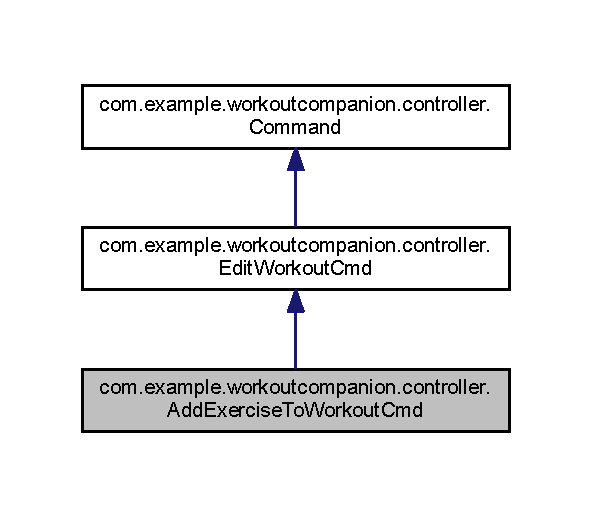
\includegraphics[width=284pt]{classcom_1_1example_1_1workoutcompanion_1_1controller_1_1_add_exercise_to_workout_cmd__inherit__graph}
\end{center}
\end{figure}


Collaboration diagram for com.\-example.\-workoutcompanion.\-controller.\-Add\-Exercise\-To\-Workout\-Cmd\-:
\nopagebreak
\begin{figure}[H]
\begin{center}
\leavevmode
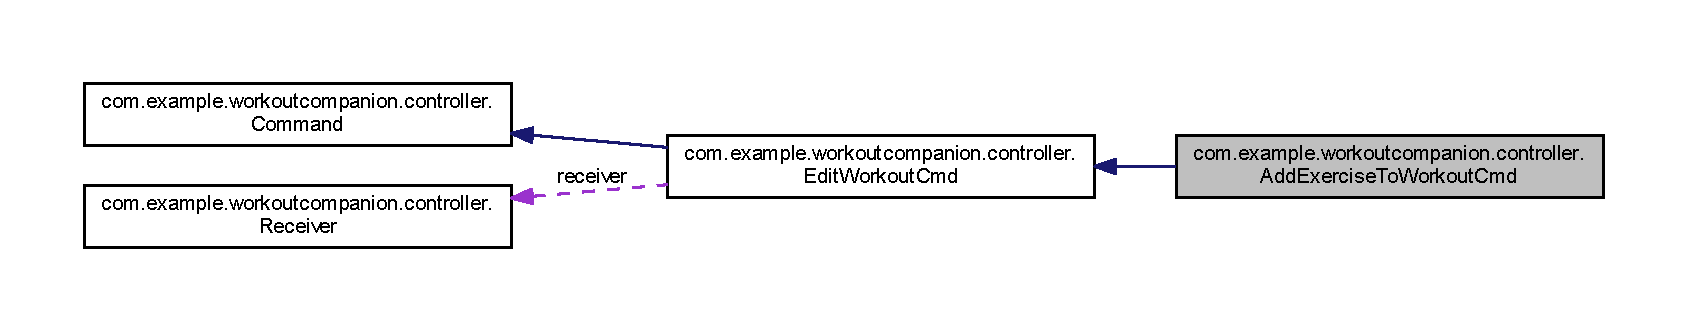
\includegraphics[width=350pt]{classcom_1_1example_1_1workoutcompanion_1_1controller_1_1_add_exercise_to_workout_cmd__coll__graph}
\end{center}
\end{figure}
\subsection*{Public Member Functions}
\begin{DoxyCompactItemize}
\item 
\hyperlink{classcom_1_1example_1_1workoutcompanion_1_1controller_1_1_add_exercise_to_workout_cmd_a99eead165db3c00c198ce107bbdc743e}{Add\-Exercise\-To\-Workout\-Cmd} (\hyperlink{classcom_1_1example_1_1workoutcompanion_1_1controller_1_1_receiver}{Receiver} receiver)
\item 
void \hyperlink{classcom_1_1example_1_1workoutcompanion_1_1controller_1_1_add_exercise_to_workout_cmd_a2e060976cc87dc386e97a8cb81fecaa2}{execute} (String...\-names)
\end{DoxyCompactItemize}


\subsection{Constructor \& Destructor Documentation}
\hypertarget{classcom_1_1example_1_1workoutcompanion_1_1controller_1_1_add_exercise_to_workout_cmd_a99eead165db3c00c198ce107bbdc743e}{\index{com\-::example\-::workoutcompanion\-::controller\-::\-Add\-Exercise\-To\-Workout\-Cmd@{com\-::example\-::workoutcompanion\-::controller\-::\-Add\-Exercise\-To\-Workout\-Cmd}!Add\-Exercise\-To\-Workout\-Cmd@{Add\-Exercise\-To\-Workout\-Cmd}}
\index{Add\-Exercise\-To\-Workout\-Cmd@{Add\-Exercise\-To\-Workout\-Cmd}!com::example::workoutcompanion::controller::AddExerciseToWorkoutCmd@{com\-::example\-::workoutcompanion\-::controller\-::\-Add\-Exercise\-To\-Workout\-Cmd}}
\subsubsection[{Add\-Exercise\-To\-Workout\-Cmd}]{\setlength{\rightskip}{0pt plus 5cm}com.\-example.\-workoutcompanion.\-controller.\-Add\-Exercise\-To\-Workout\-Cmd.\-Add\-Exercise\-To\-Workout\-Cmd (
\begin{DoxyParamCaption}
\item[{{\bf Receiver}}]{receiver}
\end{DoxyParamCaption}
)}}\label{classcom_1_1example_1_1workoutcompanion_1_1controller_1_1_add_exercise_to_workout_cmd_a99eead165db3c00c198ce107bbdc743e}


\subsection{Member Function Documentation}
\hypertarget{classcom_1_1example_1_1workoutcompanion_1_1controller_1_1_add_exercise_to_workout_cmd_a2e060976cc87dc386e97a8cb81fecaa2}{\index{com\-::example\-::workoutcompanion\-::controller\-::\-Add\-Exercise\-To\-Workout\-Cmd@{com\-::example\-::workoutcompanion\-::controller\-::\-Add\-Exercise\-To\-Workout\-Cmd}!execute@{execute}}
\index{execute@{execute}!com::example::workoutcompanion::controller::AddExerciseToWorkoutCmd@{com\-::example\-::workoutcompanion\-::controller\-::\-Add\-Exercise\-To\-Workout\-Cmd}}
\subsubsection[{execute}]{\setlength{\rightskip}{0pt plus 5cm}void com.\-example.\-workoutcompanion.\-controller.\-Add\-Exercise\-To\-Workout\-Cmd.\-execute (
\begin{DoxyParamCaption}
\item[{String...}]{names}
\end{DoxyParamCaption}
)}}\label{classcom_1_1example_1_1workoutcompanion_1_1controller_1_1_add_exercise_to_workout_cmd_a2e060976cc87dc386e97a8cb81fecaa2}


Implements \hyperlink{interfacecom_1_1example_1_1workoutcompanion_1_1controller_1_1_command_ad947864c82a300557eed99dd8367c020}{com.\-example.\-workoutcompanion.\-controller.\-Command}.



The documentation for this class was generated from the following file\-:\begin{DoxyCompactItemize}
\item 
Desktop/git\-\_\-proj/workout/src/com/example/workoutcompanion/controller/\hyperlink{_add_exercise_to_workout_cmd_8java}{Add\-Exercise\-To\-Workout\-Cmd.\-java}\end{DoxyCompactItemize}

\hypertarget{classcom_1_1example_1_1workoutcompanion_1_1_build_config}{\section{com.\-example.\-workoutcompanion.\-Build\-Config Class Reference}
\label{classcom_1_1example_1_1workoutcompanion_1_1_build_config}\index{com.\-example.\-workoutcompanion.\-Build\-Config@{com.\-example.\-workoutcompanion.\-Build\-Config}}
}
\subsection*{Static Public Attributes}
\begin{DoxyCompactItemize}
\item 
static final boolean \hyperlink{classcom_1_1example_1_1workoutcompanion_1_1_build_config_ae965e9b7606aa3b310518a23056acca0}{D\-E\-B\-U\-G} = true
\end{DoxyCompactItemize}


\subsection{Member Data Documentation}
\hypertarget{classcom_1_1example_1_1workoutcompanion_1_1_build_config_ae965e9b7606aa3b310518a23056acca0}{\index{com\-::example\-::workoutcompanion\-::\-Build\-Config@{com\-::example\-::workoutcompanion\-::\-Build\-Config}!D\-E\-B\-U\-G@{D\-E\-B\-U\-G}}
\index{D\-E\-B\-U\-G@{D\-E\-B\-U\-G}!com::example::workoutcompanion::BuildConfig@{com\-::example\-::workoutcompanion\-::\-Build\-Config}}
\subsubsection[{D\-E\-B\-U\-G}]{\setlength{\rightskip}{0pt plus 5cm}final boolean com.\-example.\-workoutcompanion.\-Build\-Config.\-D\-E\-B\-U\-G = true\hspace{0.3cm}{\ttfamily [static]}}}\label{classcom_1_1example_1_1workoutcompanion_1_1_build_config_ae965e9b7606aa3b310518a23056acca0}


The documentation for this class was generated from the following file\-:\begin{DoxyCompactItemize}
\item 
Desktop/git\-\_\-proj/workout/gen/com/example/workoutcompanion/\hyperlink{_build_config_8java}{Build\-Config.\-java}\end{DoxyCompactItemize}

\hypertarget{interfacecom_1_1example_1_1workoutcompanion_1_1controller_1_1_command}{\section{com.\-example.\-workoutcompanion.\-controller.\-Command Interface Reference}
\label{interfacecom_1_1example_1_1workoutcompanion_1_1controller_1_1_command}\index{com.\-example.\-workoutcompanion.\-controller.\-Command@{com.\-example.\-workoutcompanion.\-controller.\-Command}}
}


Inheritance diagram for com.\-example.\-workoutcompanion.\-controller.\-Command\-:\nopagebreak
\begin{figure}[H]
\begin{center}
\leavevmode
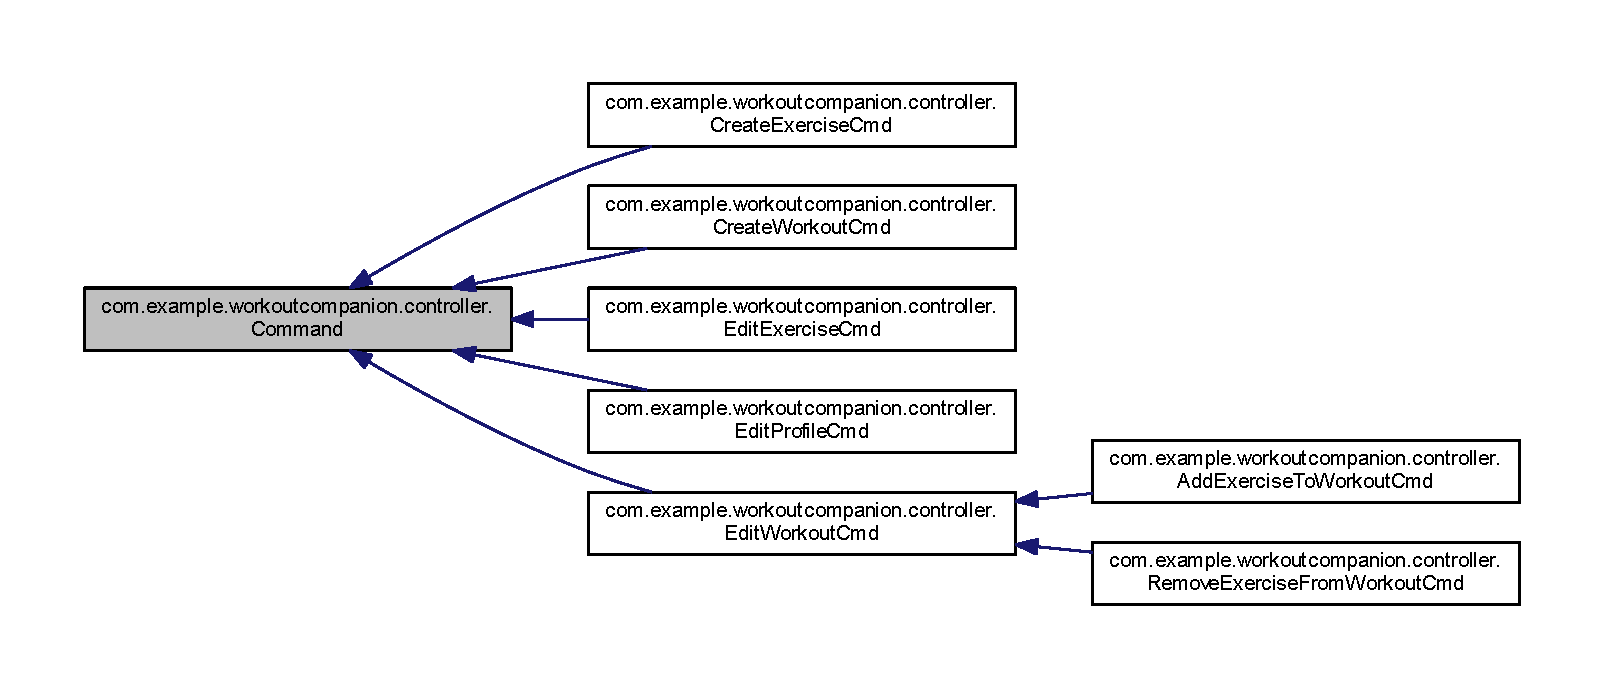
\includegraphics[width=350pt]{interfacecom_1_1example_1_1workoutcompanion_1_1controller_1_1_command__inherit__graph}
\end{center}
\end{figure}
\subsection*{Public Member Functions}
\begin{DoxyCompactItemize}
\item 
void \hyperlink{interfacecom_1_1example_1_1workoutcompanion_1_1controller_1_1_command_ad947864c82a300557eed99dd8367c020}{execute} (String...\-names)
\end{DoxyCompactItemize}


\subsection{Detailed Description}
\hyperlink{interfacecom_1_1example_1_1workoutcompanion_1_1controller_1_1_command}{Command} interface 

\subsection{Member Function Documentation}
\hypertarget{interfacecom_1_1example_1_1workoutcompanion_1_1controller_1_1_command_ad947864c82a300557eed99dd8367c020}{\index{com\-::example\-::workoutcompanion\-::controller\-::\-Command@{com\-::example\-::workoutcompanion\-::controller\-::\-Command}!execute@{execute}}
\index{execute@{execute}!com::example::workoutcompanion::controller::Command@{com\-::example\-::workoutcompanion\-::controller\-::\-Command}}
\subsubsection[{execute}]{\setlength{\rightskip}{0pt plus 5cm}void com.\-example.\-workoutcompanion.\-controller.\-Command.\-execute (
\begin{DoxyParamCaption}
\item[{String...}]{names}
\end{DoxyParamCaption}
)}}\label{interfacecom_1_1example_1_1workoutcompanion_1_1controller_1_1_command_ad947864c82a300557eed99dd8367c020}


Implemented in \hyperlink{classcom_1_1example_1_1workoutcompanion_1_1controller_1_1_create_workout_cmd_a40658da724258d7d017d73d10c010396}{com.\-example.\-workoutcompanion.\-controller.\-Create\-Workout\-Cmd}, \hyperlink{classcom_1_1example_1_1workoutcompanion_1_1controller_1_1_edit_exercise_cmd_ad88895b70ef7059ee016b328c935fa9d}{com.\-example.\-workoutcompanion.\-controller.\-Edit\-Exercise\-Cmd}, \hyperlink{classcom_1_1example_1_1workoutcompanion_1_1controller_1_1_edit_profile_cmd_aa88c4baa3aa144886cfe457c8eb270ff}{com.\-example.\-workoutcompanion.\-controller.\-Edit\-Profile\-Cmd}, \hyperlink{classcom_1_1example_1_1workoutcompanion_1_1controller_1_1_add_exercise_to_workout_cmd_a2e060976cc87dc386e97a8cb81fecaa2}{com.\-example.\-workoutcompanion.\-controller.\-Add\-Exercise\-To\-Workout\-Cmd}, \hyperlink{classcom_1_1example_1_1workoutcompanion_1_1controller_1_1_create_exercise_cmd_a54780641f2d350f4f8ce9dd124938425}{com.\-example.\-workoutcompanion.\-controller.\-Create\-Exercise\-Cmd}, and \hyperlink{classcom_1_1example_1_1workoutcompanion_1_1controller_1_1_remove_exercise_from_workout_cmd_aa1212feda70af3ae8eb41f2a47fc38e8}{com.\-example.\-workoutcompanion.\-controller.\-Remove\-Exercise\-From\-Workout\-Cmd}.



The documentation for this interface was generated from the following file\-:\begin{DoxyCompactItemize}
\item 
Desktop/git\-\_\-proj/workout/src/com/example/workoutcompanion/controller/\hyperlink{_command_8java}{Command.\-java}\end{DoxyCompactItemize}

\hypertarget{classcom_1_1example_1_1workoutcompanion_1_1controller_1_1_controller}{\section{com.\-example.\-workoutcompanion.\-controller.\-Controller Class Reference}
\label{classcom_1_1example_1_1workoutcompanion_1_1controller_1_1_controller}\index{com.\-example.\-workoutcompanion.\-controller.\-Controller@{com.\-example.\-workoutcompanion.\-controller.\-Controller}}
}
\subsection*{Public Member Functions}
\begin{DoxyCompactItemize}
\item 
\hyperlink{classcom_1_1example_1_1workoutcompanion_1_1controller_1_1_controller_aad923fda94f125fee5009e529ef1ac6d}{Controller} (Context context)
\end{DoxyCompactItemize}


\subsection{Constructor \& Destructor Documentation}
\hypertarget{classcom_1_1example_1_1workoutcompanion_1_1controller_1_1_controller_aad923fda94f125fee5009e529ef1ac6d}{\index{com\-::example\-::workoutcompanion\-::controller\-::\-Controller@{com\-::example\-::workoutcompanion\-::controller\-::\-Controller}!Controller@{Controller}}
\index{Controller@{Controller}!com::example::workoutcompanion::controller::Controller@{com\-::example\-::workoutcompanion\-::controller\-::\-Controller}}
\subsubsection[{Controller}]{\setlength{\rightskip}{0pt plus 5cm}com.\-example.\-workoutcompanion.\-controller.\-Controller.\-Controller (
\begin{DoxyParamCaption}
\item[{Context}]{context}
\end{DoxyParamCaption}
)}}\label{classcom_1_1example_1_1workoutcompanion_1_1controller_1_1_controller_aad923fda94f125fee5009e529ef1ac6d}


The documentation for this class was generated from the following file\-:\begin{DoxyCompactItemize}
\item 
Desktop/git\-\_\-proj/workout/src/com/example/workoutcompanion/controller/\hyperlink{_controller_8java}{Controller.\-java}\end{DoxyCompactItemize}

\hypertarget{classcom_1_1example_1_1workoutcompanion_1_1controller_1_1_create_exercise_cmd}{\section{com.\-example.\-workoutcompanion.\-controller.\-Create\-Exercise\-Cmd Class Reference}
\label{classcom_1_1example_1_1workoutcompanion_1_1controller_1_1_create_exercise_cmd}\index{com.\-example.\-workoutcompanion.\-controller.\-Create\-Exercise\-Cmd@{com.\-example.\-workoutcompanion.\-controller.\-Create\-Exercise\-Cmd}}
}


Inheritance diagram for com.\-example.\-workoutcompanion.\-controller.\-Create\-Exercise\-Cmd\-:\nopagebreak
\begin{figure}[H]
\begin{center}
\leavevmode
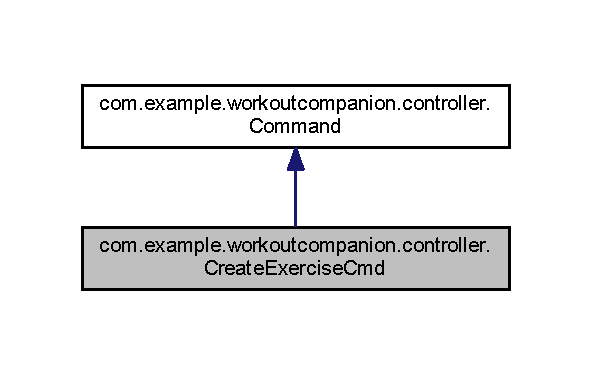
\includegraphics[width=284pt]{classcom_1_1example_1_1workoutcompanion_1_1controller_1_1_create_exercise_cmd__inherit__graph}
\end{center}
\end{figure}


Collaboration diagram for com.\-example.\-workoutcompanion.\-controller.\-Create\-Exercise\-Cmd\-:\nopagebreak
\begin{figure}[H]
\begin{center}
\leavevmode
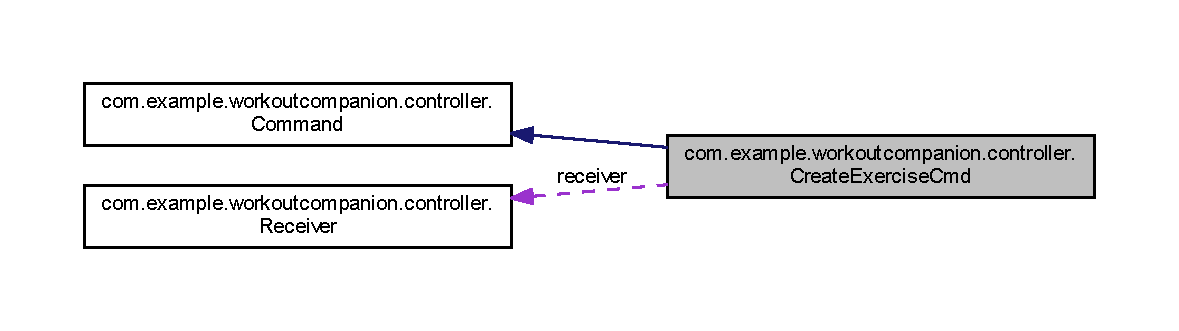
\includegraphics[width=350pt]{classcom_1_1example_1_1workoutcompanion_1_1controller_1_1_create_exercise_cmd__coll__graph}
\end{center}
\end{figure}
\subsection*{Public Member Functions}
\begin{DoxyCompactItemize}
\item 
\hyperlink{classcom_1_1example_1_1workoutcompanion_1_1controller_1_1_create_exercise_cmd_a429408763986cc4d27ef3d1b3faff69b}{Create\-Exercise\-Cmd} (\hyperlink{classcom_1_1example_1_1workoutcompanion_1_1controller_1_1_receiver}{Receiver} receiver)
\item 
void \hyperlink{classcom_1_1example_1_1workoutcompanion_1_1controller_1_1_create_exercise_cmd_a54780641f2d350f4f8ce9dd124938425}{execute} (String...\-names)
\end{DoxyCompactItemize}


\subsection{Constructor \& Destructor Documentation}
\hypertarget{classcom_1_1example_1_1workoutcompanion_1_1controller_1_1_create_exercise_cmd_a429408763986cc4d27ef3d1b3faff69b}{\index{com\-::example\-::workoutcompanion\-::controller\-::\-Create\-Exercise\-Cmd@{com\-::example\-::workoutcompanion\-::controller\-::\-Create\-Exercise\-Cmd}!Create\-Exercise\-Cmd@{Create\-Exercise\-Cmd}}
\index{Create\-Exercise\-Cmd@{Create\-Exercise\-Cmd}!com::example::workoutcompanion::controller::CreateExerciseCmd@{com\-::example\-::workoutcompanion\-::controller\-::\-Create\-Exercise\-Cmd}}
\subsubsection[{Create\-Exercise\-Cmd}]{\setlength{\rightskip}{0pt plus 5cm}com.\-example.\-workoutcompanion.\-controller.\-Create\-Exercise\-Cmd.\-Create\-Exercise\-Cmd (
\begin{DoxyParamCaption}
\item[{{\bf Receiver}}]{receiver}
\end{DoxyParamCaption}
)}}\label{classcom_1_1example_1_1workoutcompanion_1_1controller_1_1_create_exercise_cmd_a429408763986cc4d27ef3d1b3faff69b}


\subsection{Member Function Documentation}
\hypertarget{classcom_1_1example_1_1workoutcompanion_1_1controller_1_1_create_exercise_cmd_a54780641f2d350f4f8ce9dd124938425}{\index{com\-::example\-::workoutcompanion\-::controller\-::\-Create\-Exercise\-Cmd@{com\-::example\-::workoutcompanion\-::controller\-::\-Create\-Exercise\-Cmd}!execute@{execute}}
\index{execute@{execute}!com::example::workoutcompanion::controller::CreateExerciseCmd@{com\-::example\-::workoutcompanion\-::controller\-::\-Create\-Exercise\-Cmd}}
\subsubsection[{execute}]{\setlength{\rightskip}{0pt plus 5cm}void com.\-example.\-workoutcompanion.\-controller.\-Create\-Exercise\-Cmd.\-execute (
\begin{DoxyParamCaption}
\item[{String...}]{names}
\end{DoxyParamCaption}
)}}\label{classcom_1_1example_1_1workoutcompanion_1_1controller_1_1_create_exercise_cmd_a54780641f2d350f4f8ce9dd124938425}


Implements \hyperlink{interfacecom_1_1example_1_1workoutcompanion_1_1controller_1_1_command_ad947864c82a300557eed99dd8367c020}{com.\-example.\-workoutcompanion.\-controller.\-Command}.



The documentation for this class was generated from the following file\-:\begin{DoxyCompactItemize}
\item 
Desktop/git\-\_\-proj/workout/src/com/example/workoutcompanion/controller/\hyperlink{_create_exercise_cmd_8java}{Create\-Exercise\-Cmd.\-java}\end{DoxyCompactItemize}

\hypertarget{classcom_1_1example_1_1workoutcompanion_1_1controller_1_1_create_workout_cmd}{\section{com.\-example.\-workoutcompanion.\-controller.\-Create\-Workout\-Cmd Class Reference}
\label{classcom_1_1example_1_1workoutcompanion_1_1controller_1_1_create_workout_cmd}\index{com.\-example.\-workoutcompanion.\-controller.\-Create\-Workout\-Cmd@{com.\-example.\-workoutcompanion.\-controller.\-Create\-Workout\-Cmd}}
}


Inheritance diagram for com.\-example.\-workoutcompanion.\-controller.\-Create\-Workout\-Cmd\-:
\nopagebreak
\begin{figure}[H]
\begin{center}
\leavevmode
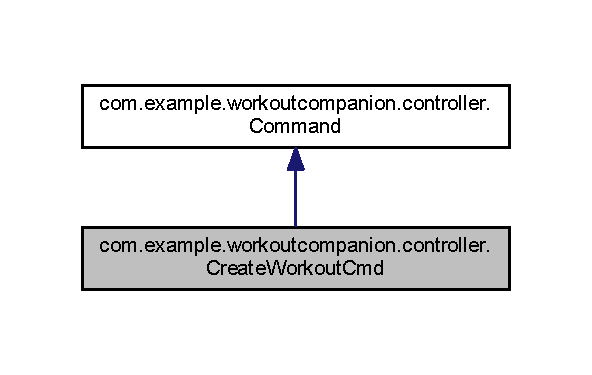
\includegraphics[width=284pt]{classcom_1_1example_1_1workoutcompanion_1_1controller_1_1_create_workout_cmd__inherit__graph}
\end{center}
\end{figure}


Collaboration diagram for com.\-example.\-workoutcompanion.\-controller.\-Create\-Workout\-Cmd\-:
\nopagebreak
\begin{figure}[H]
\begin{center}
\leavevmode
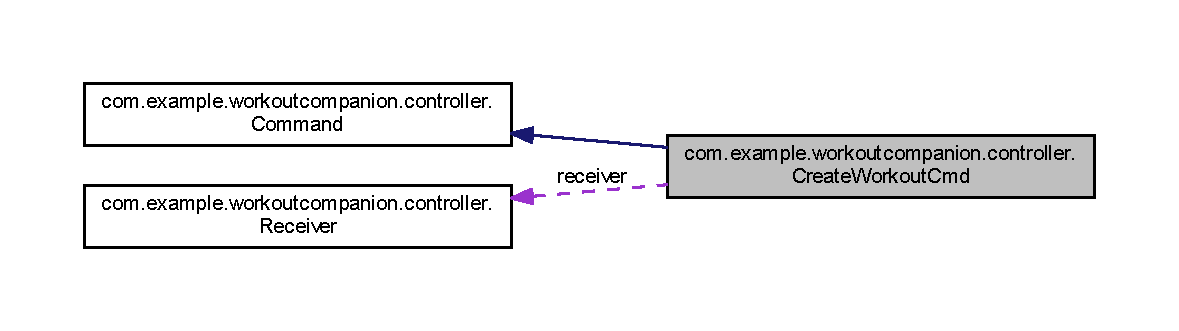
\includegraphics[width=350pt]{classcom_1_1example_1_1workoutcompanion_1_1controller_1_1_create_workout_cmd__coll__graph}
\end{center}
\end{figure}
\subsection*{Public Member Functions}
\begin{DoxyCompactItemize}
\item 
\hyperlink{classcom_1_1example_1_1workoutcompanion_1_1controller_1_1_create_workout_cmd_a55e5031af6d0106d82c050ddf68b9128}{Create\-Workout\-Cmd} (\hyperlink{classcom_1_1example_1_1workoutcompanion_1_1controller_1_1_receiver}{Receiver} receiver)
\item 
void \hyperlink{classcom_1_1example_1_1workoutcompanion_1_1controller_1_1_create_workout_cmd_a40658da724258d7d017d73d10c010396}{execute} (String...\-names)
\end{DoxyCompactItemize}


\subsection{Constructor \& Destructor Documentation}
\hypertarget{classcom_1_1example_1_1workoutcompanion_1_1controller_1_1_create_workout_cmd_a55e5031af6d0106d82c050ddf68b9128}{\index{com\-::example\-::workoutcompanion\-::controller\-::\-Create\-Workout\-Cmd@{com\-::example\-::workoutcompanion\-::controller\-::\-Create\-Workout\-Cmd}!Create\-Workout\-Cmd@{Create\-Workout\-Cmd}}
\index{Create\-Workout\-Cmd@{Create\-Workout\-Cmd}!com::example::workoutcompanion::controller::CreateWorkoutCmd@{com\-::example\-::workoutcompanion\-::controller\-::\-Create\-Workout\-Cmd}}
\subsubsection[{Create\-Workout\-Cmd}]{\setlength{\rightskip}{0pt plus 5cm}com.\-example.\-workoutcompanion.\-controller.\-Create\-Workout\-Cmd.\-Create\-Workout\-Cmd (
\begin{DoxyParamCaption}
\item[{{\bf Receiver}}]{receiver}
\end{DoxyParamCaption}
)}}\label{classcom_1_1example_1_1workoutcompanion_1_1controller_1_1_create_workout_cmd_a55e5031af6d0106d82c050ddf68b9128}


\subsection{Member Function Documentation}
\hypertarget{classcom_1_1example_1_1workoutcompanion_1_1controller_1_1_create_workout_cmd_a40658da724258d7d017d73d10c010396}{\index{com\-::example\-::workoutcompanion\-::controller\-::\-Create\-Workout\-Cmd@{com\-::example\-::workoutcompanion\-::controller\-::\-Create\-Workout\-Cmd}!execute@{execute}}
\index{execute@{execute}!com::example::workoutcompanion::controller::CreateWorkoutCmd@{com\-::example\-::workoutcompanion\-::controller\-::\-Create\-Workout\-Cmd}}
\subsubsection[{execute}]{\setlength{\rightskip}{0pt plus 5cm}void com.\-example.\-workoutcompanion.\-controller.\-Create\-Workout\-Cmd.\-execute (
\begin{DoxyParamCaption}
\item[{String...}]{names}
\end{DoxyParamCaption}
)}}\label{classcom_1_1example_1_1workoutcompanion_1_1controller_1_1_create_workout_cmd_a40658da724258d7d017d73d10c010396}
names\mbox{[}0\mbox{]} -\/ name of the workout names\mbox{[}...\mbox{]} -\/ names of workouts 

Implements \hyperlink{interfacecom_1_1example_1_1workoutcompanion_1_1controller_1_1_command_ad947864c82a300557eed99dd8367c020}{com.\-example.\-workoutcompanion.\-controller.\-Command}.



The documentation for this class was generated from the following file\-:\begin{DoxyCompactItemize}
\item 
Desktop/git\-\_\-proj/workout/src/com/example/workoutcompanion/controller/\hyperlink{_create_workout_cmd_8java}{Create\-Workout\-Cmd.\-java}\end{DoxyCompactItemize}

\hypertarget{classcom_1_1example_1_1workoutcompanion_1_1db_1_1_database_handler}{\section{com.\-example.\-workoutcompanion.\-db.\-Database\-Handler Class Reference}
\label{classcom_1_1example_1_1workoutcompanion_1_1db_1_1_database_handler}\index{com.\-example.\-workoutcompanion.\-db.\-Database\-Handler@{com.\-example.\-workoutcompanion.\-db.\-Database\-Handler}}
}


Inheritance diagram for com.\-example.\-workoutcompanion.\-db.\-Database\-Handler\-:\nopagebreak
\begin{figure}[H]
\begin{center}
\leavevmode
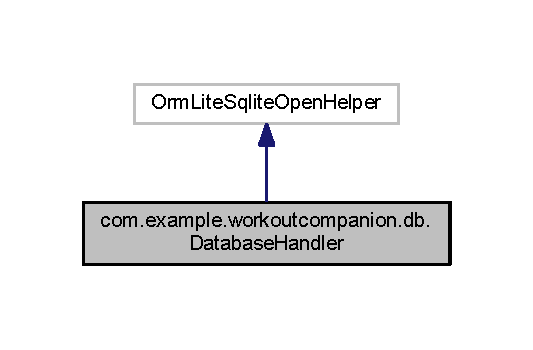
\includegraphics[width=256pt]{classcom_1_1example_1_1workoutcompanion_1_1db_1_1_database_handler__inherit__graph}
\end{center}
\end{figure}


Collaboration diagram for com.\-example.\-workoutcompanion.\-db.\-Database\-Handler\-:\nopagebreak
\begin{figure}[H]
\begin{center}
\leavevmode
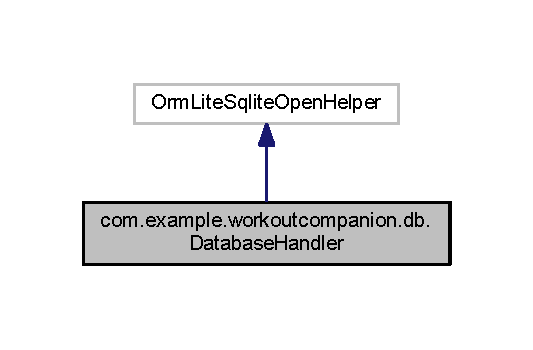
\includegraphics[width=256pt]{classcom_1_1example_1_1workoutcompanion_1_1db_1_1_database_handler__coll__graph}
\end{center}
\end{figure}
\subsection*{Public Member Functions}
\begin{DoxyCompactItemize}
\item 
\hyperlink{classcom_1_1example_1_1workoutcompanion_1_1db_1_1_database_handler_a70557f69e2eed6ec8a586c57ad6c5148}{Database\-Handler} (Context a\-Context)
\item 
void \hyperlink{classcom_1_1example_1_1workoutcompanion_1_1db_1_1_database_handler_ae8b1c67a6abc49ee420227fa24d54420}{on\-Create} (S\-Q\-Lite\-Database arg0, Connection\-Source arg1)
\item 
void \hyperlink{classcom_1_1example_1_1workoutcompanion_1_1db_1_1_database_handler_ac806115da11f781668b749a3c73e645b}{on\-Upgrade} (S\-Q\-Lite\-Database arg0, Connection\-Source arg1, int arg2, int arg3)
\item 
void \hyperlink{classcom_1_1example_1_1workoutcompanion_1_1db_1_1_database_handler_a89c6c6effa783f1873ebbcb9b301c6d8}{close} ()
\item 
\hyperlink{classcom_1_1example_1_1workoutcompanion_1_1dom_1_1_workout}{Workout} \hyperlink{classcom_1_1example_1_1workoutcompanion_1_1db_1_1_database_handler_aad77efaa1ca2fecbac8ef4b0c283fa12}{find\-Workout} (String workout\-Name)  throws S\-Q\-L\-Exception 
\item 
List$<$ \hyperlink{classcom_1_1example_1_1workoutcompanion_1_1dom_1_1_workout}{Workout} $>$ \hyperlink{classcom_1_1example_1_1workoutcompanion_1_1db_1_1_database_handler_a0375493d23c0dd16988f5b375b87be9b}{find\-All\-Workouts} ()  throws S\-Q\-L\-Exception 
\item 
\hyperlink{classcom_1_1example_1_1workoutcompanion_1_1dom_1_1_exercise}{Exercise} \hyperlink{classcom_1_1example_1_1workoutcompanion_1_1db_1_1_database_handler_af529635c9fad7b21b1f2afb17a0ca17f}{find\-Exercise} (String exercise\-Name)  throws S\-Q\-L\-Exception 
\item 
\hyperlink{classcom_1_1example_1_1workoutcompanion_1_1dom_1_1_exercise}{Exercise} \hyperlink{classcom_1_1example_1_1workoutcompanion_1_1db_1_1_database_handler_aa6f903c2616f7863bdf5199d43d955d3}{change\-Exercise\-Name} (String old\-Name, String new\-Name)  throws S\-Q\-L\-Exception 
\item 
\hyperlink{classcom_1_1example_1_1workoutcompanion_1_1dom_1_1_workout}{Workout} \hyperlink{classcom_1_1example_1_1workoutcompanion_1_1db_1_1_database_handler_acbc08344a1d529bfee3ff7c159126511}{change\-Workout\-Name} (String old\-Name, String new\-Name)  throws S\-Q\-L\-Exception 
\item 
List$<$ \hyperlink{classcom_1_1example_1_1workoutcompanion_1_1dom_1_1_exercise}{Exercise} $>$ \hyperlink{classcom_1_1example_1_1workoutcompanion_1_1db_1_1_database_handler_ac4159f5b8abd44ac948ef74031a7e7cc}{find\-All\-Exercises} ()  throws S\-Q\-L\-Exception 
\item 
\hyperlink{classcom_1_1example_1_1workoutcompanion_1_1dom_1_1_workout}{Workout} \hyperlink{classcom_1_1example_1_1workoutcompanion_1_1db_1_1_database_handler_a7677c50b7f83e38b29c61e4c63a90eef}{add\-Or\-Update\-Workout} (\hyperlink{classcom_1_1example_1_1workoutcompanion_1_1dom_1_1_workout}{Workout} a\-Workout)  throws S\-Q\-L\-Exception 
\item 
\hyperlink{classcom_1_1example_1_1workoutcompanion_1_1dom_1_1_exercise}{Exercise} \hyperlink{classcom_1_1example_1_1workoutcompanion_1_1db_1_1_database_handler_ad16c1da657957572cb436dc4b162814b}{add\-Or\-Update\-Exercise} (\hyperlink{classcom_1_1example_1_1workoutcompanion_1_1dom_1_1_exercise}{Exercise} a\-Exercise)  throws S\-Q\-L\-Exception 
\item 
void \hyperlink{classcom_1_1example_1_1workoutcompanion_1_1db_1_1_database_handler_a1b6c0537995132d282b71ffabdccb319}{remove\-Workout} (String name)  throws S\-Q\-L\-Exception 
\item 
void \hyperlink{classcom_1_1example_1_1workoutcompanion_1_1db_1_1_database_handler_ada07c0d3c047c761fde4e75832f5a6d9}{remove\-Exercise} (String name)  throws S\-Q\-L\-Exception 
\end{DoxyCompactItemize}


\subsection{Constructor \& Destructor Documentation}
\hypertarget{classcom_1_1example_1_1workoutcompanion_1_1db_1_1_database_handler_a70557f69e2eed6ec8a586c57ad6c5148}{\index{com\-::example\-::workoutcompanion\-::db\-::\-Database\-Handler@{com\-::example\-::workoutcompanion\-::db\-::\-Database\-Handler}!Database\-Handler@{Database\-Handler}}
\index{Database\-Handler@{Database\-Handler}!com::example::workoutcompanion::db::DatabaseHandler@{com\-::example\-::workoutcompanion\-::db\-::\-Database\-Handler}}
\subsubsection[{Database\-Handler}]{\setlength{\rightskip}{0pt plus 5cm}com.\-example.\-workoutcompanion.\-db.\-Database\-Handler.\-Database\-Handler (
\begin{DoxyParamCaption}
\item[{Context}]{a\-Context}
\end{DoxyParamCaption}
)}}\label{classcom_1_1example_1_1workoutcompanion_1_1db_1_1_database_handler_a70557f69e2eed6ec8a586c57ad6c5148}


\subsection{Member Function Documentation}
\hypertarget{classcom_1_1example_1_1workoutcompanion_1_1db_1_1_database_handler_ad16c1da657957572cb436dc4b162814b}{\index{com\-::example\-::workoutcompanion\-::db\-::\-Database\-Handler@{com\-::example\-::workoutcompanion\-::db\-::\-Database\-Handler}!add\-Or\-Update\-Exercise@{add\-Or\-Update\-Exercise}}
\index{add\-Or\-Update\-Exercise@{add\-Or\-Update\-Exercise}!com::example::workoutcompanion::db::DatabaseHandler@{com\-::example\-::workoutcompanion\-::db\-::\-Database\-Handler}}
\subsubsection[{add\-Or\-Update\-Exercise}]{\setlength{\rightskip}{0pt plus 5cm}{\bf Exercise} com.\-example.\-workoutcompanion.\-db.\-Database\-Handler.\-add\-Or\-Update\-Exercise (
\begin{DoxyParamCaption}
\item[{{\bf Exercise}}]{a\-Exercise}
\end{DoxyParamCaption}
) throws S\-Q\-L\-Exception}}\label{classcom_1_1example_1_1workoutcompanion_1_1db_1_1_database_handler_ad16c1da657957572cb436dc4b162814b}
\hypertarget{classcom_1_1example_1_1workoutcompanion_1_1db_1_1_database_handler_a7677c50b7f83e38b29c61e4c63a90eef}{\index{com\-::example\-::workoutcompanion\-::db\-::\-Database\-Handler@{com\-::example\-::workoutcompanion\-::db\-::\-Database\-Handler}!add\-Or\-Update\-Workout@{add\-Or\-Update\-Workout}}
\index{add\-Or\-Update\-Workout@{add\-Or\-Update\-Workout}!com::example::workoutcompanion::db::DatabaseHandler@{com\-::example\-::workoutcompanion\-::db\-::\-Database\-Handler}}
\subsubsection[{add\-Or\-Update\-Workout}]{\setlength{\rightskip}{0pt plus 5cm}{\bf Workout} com.\-example.\-workoutcompanion.\-db.\-Database\-Handler.\-add\-Or\-Update\-Workout (
\begin{DoxyParamCaption}
\item[{{\bf Workout}}]{a\-Workout}
\end{DoxyParamCaption}
) throws S\-Q\-L\-Exception}}\label{classcom_1_1example_1_1workoutcompanion_1_1db_1_1_database_handler_a7677c50b7f83e38b29c61e4c63a90eef}
\hypertarget{classcom_1_1example_1_1workoutcompanion_1_1db_1_1_database_handler_aa6f903c2616f7863bdf5199d43d955d3}{\index{com\-::example\-::workoutcompanion\-::db\-::\-Database\-Handler@{com\-::example\-::workoutcompanion\-::db\-::\-Database\-Handler}!change\-Exercise\-Name@{change\-Exercise\-Name}}
\index{change\-Exercise\-Name@{change\-Exercise\-Name}!com::example::workoutcompanion::db::DatabaseHandler@{com\-::example\-::workoutcompanion\-::db\-::\-Database\-Handler}}
\subsubsection[{change\-Exercise\-Name}]{\setlength{\rightskip}{0pt plus 5cm}{\bf Exercise} com.\-example.\-workoutcompanion.\-db.\-Database\-Handler.\-change\-Exercise\-Name (
\begin{DoxyParamCaption}
\item[{String}]{old\-Name, }
\item[{String}]{new\-Name}
\end{DoxyParamCaption}
) throws S\-Q\-L\-Exception}}\label{classcom_1_1example_1_1workoutcompanion_1_1db_1_1_database_handler_aa6f903c2616f7863bdf5199d43d955d3}
\hypertarget{classcom_1_1example_1_1workoutcompanion_1_1db_1_1_database_handler_acbc08344a1d529bfee3ff7c159126511}{\index{com\-::example\-::workoutcompanion\-::db\-::\-Database\-Handler@{com\-::example\-::workoutcompanion\-::db\-::\-Database\-Handler}!change\-Workout\-Name@{change\-Workout\-Name}}
\index{change\-Workout\-Name@{change\-Workout\-Name}!com::example::workoutcompanion::db::DatabaseHandler@{com\-::example\-::workoutcompanion\-::db\-::\-Database\-Handler}}
\subsubsection[{change\-Workout\-Name}]{\setlength{\rightskip}{0pt plus 5cm}{\bf Workout} com.\-example.\-workoutcompanion.\-db.\-Database\-Handler.\-change\-Workout\-Name (
\begin{DoxyParamCaption}
\item[{String}]{old\-Name, }
\item[{String}]{new\-Name}
\end{DoxyParamCaption}
) throws S\-Q\-L\-Exception}}\label{classcom_1_1example_1_1workoutcompanion_1_1db_1_1_database_handler_acbc08344a1d529bfee3ff7c159126511}
\hypertarget{classcom_1_1example_1_1workoutcompanion_1_1db_1_1_database_handler_a89c6c6effa783f1873ebbcb9b301c6d8}{\index{com\-::example\-::workoutcompanion\-::db\-::\-Database\-Handler@{com\-::example\-::workoutcompanion\-::db\-::\-Database\-Handler}!close@{close}}
\index{close@{close}!com::example::workoutcompanion::db::DatabaseHandler@{com\-::example\-::workoutcompanion\-::db\-::\-Database\-Handler}}
\subsubsection[{close}]{\setlength{\rightskip}{0pt plus 5cm}void com.\-example.\-workoutcompanion.\-db.\-Database\-Handler.\-close (
\begin{DoxyParamCaption}
{}
\end{DoxyParamCaption}
)}}\label{classcom_1_1example_1_1workoutcompanion_1_1db_1_1_database_handler_a89c6c6effa783f1873ebbcb9b301c6d8}
Close the database connections and clear any cached D\-A\-Os. \hypertarget{classcom_1_1example_1_1workoutcompanion_1_1db_1_1_database_handler_ac4159f5b8abd44ac948ef74031a7e7cc}{\index{com\-::example\-::workoutcompanion\-::db\-::\-Database\-Handler@{com\-::example\-::workoutcompanion\-::db\-::\-Database\-Handler}!find\-All\-Exercises@{find\-All\-Exercises}}
\index{find\-All\-Exercises@{find\-All\-Exercises}!com::example::workoutcompanion::db::DatabaseHandler@{com\-::example\-::workoutcompanion\-::db\-::\-Database\-Handler}}
\subsubsection[{find\-All\-Exercises}]{\setlength{\rightskip}{0pt plus 5cm}List$<${\bf Exercise}$>$ com.\-example.\-workoutcompanion.\-db.\-Database\-Handler.\-find\-All\-Exercises (
\begin{DoxyParamCaption}
{}
\end{DoxyParamCaption}
) throws S\-Q\-L\-Exception}}\label{classcom_1_1example_1_1workoutcompanion_1_1db_1_1_database_handler_ac4159f5b8abd44ac948ef74031a7e7cc}
\hypertarget{classcom_1_1example_1_1workoutcompanion_1_1db_1_1_database_handler_a0375493d23c0dd16988f5b375b87be9b}{\index{com\-::example\-::workoutcompanion\-::db\-::\-Database\-Handler@{com\-::example\-::workoutcompanion\-::db\-::\-Database\-Handler}!find\-All\-Workouts@{find\-All\-Workouts}}
\index{find\-All\-Workouts@{find\-All\-Workouts}!com::example::workoutcompanion::db::DatabaseHandler@{com\-::example\-::workoutcompanion\-::db\-::\-Database\-Handler}}
\subsubsection[{find\-All\-Workouts}]{\setlength{\rightskip}{0pt plus 5cm}List$<${\bf Workout}$>$ com.\-example.\-workoutcompanion.\-db.\-Database\-Handler.\-find\-All\-Workouts (
\begin{DoxyParamCaption}
{}
\end{DoxyParamCaption}
) throws S\-Q\-L\-Exception}}\label{classcom_1_1example_1_1workoutcompanion_1_1db_1_1_database_handler_a0375493d23c0dd16988f5b375b87be9b}
\hypertarget{classcom_1_1example_1_1workoutcompanion_1_1db_1_1_database_handler_af529635c9fad7b21b1f2afb17a0ca17f}{\index{com\-::example\-::workoutcompanion\-::db\-::\-Database\-Handler@{com\-::example\-::workoutcompanion\-::db\-::\-Database\-Handler}!find\-Exercise@{find\-Exercise}}
\index{find\-Exercise@{find\-Exercise}!com::example::workoutcompanion::db::DatabaseHandler@{com\-::example\-::workoutcompanion\-::db\-::\-Database\-Handler}}
\subsubsection[{find\-Exercise}]{\setlength{\rightskip}{0pt plus 5cm}{\bf Exercise} com.\-example.\-workoutcompanion.\-db.\-Database\-Handler.\-find\-Exercise (
\begin{DoxyParamCaption}
\item[{String}]{exercise\-Name}
\end{DoxyParamCaption}
) throws S\-Q\-L\-Exception}}\label{classcom_1_1example_1_1workoutcompanion_1_1db_1_1_database_handler_af529635c9fad7b21b1f2afb17a0ca17f}
\hypertarget{classcom_1_1example_1_1workoutcompanion_1_1db_1_1_database_handler_aad77efaa1ca2fecbac8ef4b0c283fa12}{\index{com\-::example\-::workoutcompanion\-::db\-::\-Database\-Handler@{com\-::example\-::workoutcompanion\-::db\-::\-Database\-Handler}!find\-Workout@{find\-Workout}}
\index{find\-Workout@{find\-Workout}!com::example::workoutcompanion::db::DatabaseHandler@{com\-::example\-::workoutcompanion\-::db\-::\-Database\-Handler}}
\subsubsection[{find\-Workout}]{\setlength{\rightskip}{0pt plus 5cm}{\bf Workout} com.\-example.\-workoutcompanion.\-db.\-Database\-Handler.\-find\-Workout (
\begin{DoxyParamCaption}
\item[{String}]{workout\-Name}
\end{DoxyParamCaption}
) throws S\-Q\-L\-Exception}}\label{classcom_1_1example_1_1workoutcompanion_1_1db_1_1_database_handler_aad77efaa1ca2fecbac8ef4b0c283fa12}
\hypertarget{classcom_1_1example_1_1workoutcompanion_1_1db_1_1_database_handler_ae8b1c67a6abc49ee420227fa24d54420}{\index{com\-::example\-::workoutcompanion\-::db\-::\-Database\-Handler@{com\-::example\-::workoutcompanion\-::db\-::\-Database\-Handler}!on\-Create@{on\-Create}}
\index{on\-Create@{on\-Create}!com::example::workoutcompanion::db::DatabaseHandler@{com\-::example\-::workoutcompanion\-::db\-::\-Database\-Handler}}
\subsubsection[{on\-Create}]{\setlength{\rightskip}{0pt plus 5cm}void com.\-example.\-workoutcompanion.\-db.\-Database\-Handler.\-on\-Create (
\begin{DoxyParamCaption}
\item[{S\-Q\-Lite\-Database}]{arg0, }
\item[{Connection\-Source}]{arg1}
\end{DoxyParamCaption}
)}}\label{classcom_1_1example_1_1workoutcompanion_1_1db_1_1_database_handler_ae8b1c67a6abc49ee420227fa24d54420}
\hypertarget{classcom_1_1example_1_1workoutcompanion_1_1db_1_1_database_handler_ac806115da11f781668b749a3c73e645b}{\index{com\-::example\-::workoutcompanion\-::db\-::\-Database\-Handler@{com\-::example\-::workoutcompanion\-::db\-::\-Database\-Handler}!on\-Upgrade@{on\-Upgrade}}
\index{on\-Upgrade@{on\-Upgrade}!com::example::workoutcompanion::db::DatabaseHandler@{com\-::example\-::workoutcompanion\-::db\-::\-Database\-Handler}}
\subsubsection[{on\-Upgrade}]{\setlength{\rightskip}{0pt plus 5cm}void com.\-example.\-workoutcompanion.\-db.\-Database\-Handler.\-on\-Upgrade (
\begin{DoxyParamCaption}
\item[{S\-Q\-Lite\-Database}]{arg0, }
\item[{Connection\-Source}]{arg1, }
\item[{int}]{arg2, }
\item[{int}]{arg3}
\end{DoxyParamCaption}
)}}\label{classcom_1_1example_1_1workoutcompanion_1_1db_1_1_database_handler_ac806115da11f781668b749a3c73e645b}
\hypertarget{classcom_1_1example_1_1workoutcompanion_1_1db_1_1_database_handler_ada07c0d3c047c761fde4e75832f5a6d9}{\index{com\-::example\-::workoutcompanion\-::db\-::\-Database\-Handler@{com\-::example\-::workoutcompanion\-::db\-::\-Database\-Handler}!remove\-Exercise@{remove\-Exercise}}
\index{remove\-Exercise@{remove\-Exercise}!com::example::workoutcompanion::db::DatabaseHandler@{com\-::example\-::workoutcompanion\-::db\-::\-Database\-Handler}}
\subsubsection[{remove\-Exercise}]{\setlength{\rightskip}{0pt plus 5cm}void com.\-example.\-workoutcompanion.\-db.\-Database\-Handler.\-remove\-Exercise (
\begin{DoxyParamCaption}
\item[{String}]{name}
\end{DoxyParamCaption}
) throws S\-Q\-L\-Exception}}\label{classcom_1_1example_1_1workoutcompanion_1_1db_1_1_database_handler_ada07c0d3c047c761fde4e75832f5a6d9}
\hypertarget{classcom_1_1example_1_1workoutcompanion_1_1db_1_1_database_handler_a1b6c0537995132d282b71ffabdccb319}{\index{com\-::example\-::workoutcompanion\-::db\-::\-Database\-Handler@{com\-::example\-::workoutcompanion\-::db\-::\-Database\-Handler}!remove\-Workout@{remove\-Workout}}
\index{remove\-Workout@{remove\-Workout}!com::example::workoutcompanion::db::DatabaseHandler@{com\-::example\-::workoutcompanion\-::db\-::\-Database\-Handler}}
\subsubsection[{remove\-Workout}]{\setlength{\rightskip}{0pt plus 5cm}void com.\-example.\-workoutcompanion.\-db.\-Database\-Handler.\-remove\-Workout (
\begin{DoxyParamCaption}
\item[{String}]{name}
\end{DoxyParamCaption}
) throws S\-Q\-L\-Exception}}\label{classcom_1_1example_1_1workoutcompanion_1_1db_1_1_database_handler_a1b6c0537995132d282b71ffabdccb319}


The documentation for this class was generated from the following file\-:\begin{DoxyCompactItemize}
\item 
Desktop/git\-\_\-proj/workout/src/com/example/workoutcompanion/db/\hyperlink{_database_handler_8java}{Database\-Handler.\-java}\end{DoxyCompactItemize}

\hypertarget{classcom_1_1example_1_1workoutcompanion_1_1controller_1_1_edit_exercise_cmd}{\section{com.\-example.\-workoutcompanion.\-controller.\-Edit\-Exercise\-Cmd Class Reference}
\label{classcom_1_1example_1_1workoutcompanion_1_1controller_1_1_edit_exercise_cmd}\index{com.\-example.\-workoutcompanion.\-controller.\-Edit\-Exercise\-Cmd@{com.\-example.\-workoutcompanion.\-controller.\-Edit\-Exercise\-Cmd}}
}


Inheritance diagram for com.\-example.\-workoutcompanion.\-controller.\-Edit\-Exercise\-Cmd\-:\nopagebreak
\begin{figure}[H]
\begin{center}
\leavevmode
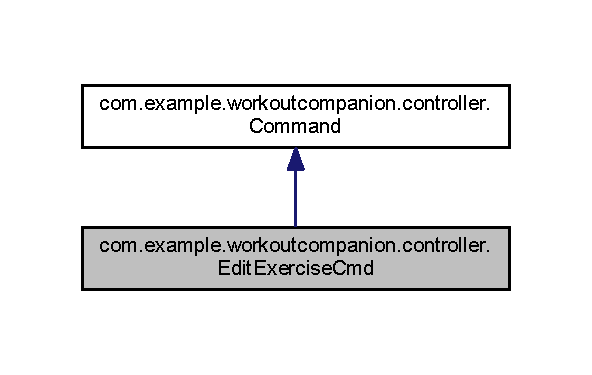
\includegraphics[width=284pt]{classcom_1_1example_1_1workoutcompanion_1_1controller_1_1_edit_exercise_cmd__inherit__graph}
\end{center}
\end{figure}


Collaboration diagram for com.\-example.\-workoutcompanion.\-controller.\-Edit\-Exercise\-Cmd\-:\nopagebreak
\begin{figure}[H]
\begin{center}
\leavevmode
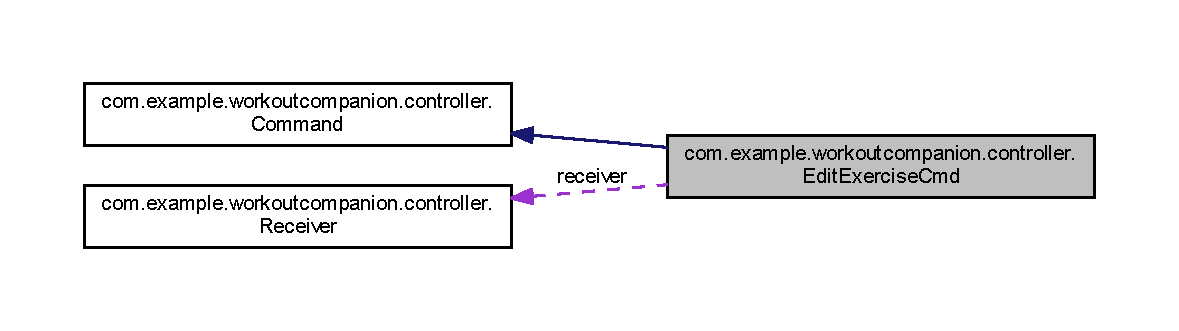
\includegraphics[width=350pt]{classcom_1_1example_1_1workoutcompanion_1_1controller_1_1_edit_exercise_cmd__coll__graph}
\end{center}
\end{figure}
\subsection*{Public Member Functions}
\begin{DoxyCompactItemize}
\item 
\hyperlink{classcom_1_1example_1_1workoutcompanion_1_1controller_1_1_edit_exercise_cmd_a69ec5e6cb3779e5ca5e99c7926208ee7}{Edit\-Exercise\-Cmd} (\hyperlink{classcom_1_1example_1_1workoutcompanion_1_1controller_1_1_receiver}{Receiver} receiver)
\item 
void \hyperlink{classcom_1_1example_1_1workoutcompanion_1_1controller_1_1_edit_exercise_cmd_ad88895b70ef7059ee016b328c935fa9d}{execute} (String...\-name)
\end{DoxyCompactItemize}


\subsection{Constructor \& Destructor Documentation}
\hypertarget{classcom_1_1example_1_1workoutcompanion_1_1controller_1_1_edit_exercise_cmd_a69ec5e6cb3779e5ca5e99c7926208ee7}{\index{com\-::example\-::workoutcompanion\-::controller\-::\-Edit\-Exercise\-Cmd@{com\-::example\-::workoutcompanion\-::controller\-::\-Edit\-Exercise\-Cmd}!Edit\-Exercise\-Cmd@{Edit\-Exercise\-Cmd}}
\index{Edit\-Exercise\-Cmd@{Edit\-Exercise\-Cmd}!com::example::workoutcompanion::controller::EditExerciseCmd@{com\-::example\-::workoutcompanion\-::controller\-::\-Edit\-Exercise\-Cmd}}
\subsubsection[{Edit\-Exercise\-Cmd}]{\setlength{\rightskip}{0pt plus 5cm}com.\-example.\-workoutcompanion.\-controller.\-Edit\-Exercise\-Cmd.\-Edit\-Exercise\-Cmd (
\begin{DoxyParamCaption}
\item[{{\bf Receiver}}]{receiver}
\end{DoxyParamCaption}
)}}\label{classcom_1_1example_1_1workoutcompanion_1_1controller_1_1_edit_exercise_cmd_a69ec5e6cb3779e5ca5e99c7926208ee7}


\subsection{Member Function Documentation}
\hypertarget{classcom_1_1example_1_1workoutcompanion_1_1controller_1_1_edit_exercise_cmd_ad88895b70ef7059ee016b328c935fa9d}{\index{com\-::example\-::workoutcompanion\-::controller\-::\-Edit\-Exercise\-Cmd@{com\-::example\-::workoutcompanion\-::controller\-::\-Edit\-Exercise\-Cmd}!execute@{execute}}
\index{execute@{execute}!com::example::workoutcompanion::controller::EditExerciseCmd@{com\-::example\-::workoutcompanion\-::controller\-::\-Edit\-Exercise\-Cmd}}
\subsubsection[{execute}]{\setlength{\rightskip}{0pt plus 5cm}void com.\-example.\-workoutcompanion.\-controller.\-Edit\-Exercise\-Cmd.\-execute (
\begin{DoxyParamCaption}
\item[{String...}]{name}
\end{DoxyParamCaption}
)}}\label{classcom_1_1example_1_1workoutcompanion_1_1controller_1_1_edit_exercise_cmd_ad88895b70ef7059ee016b328c935fa9d}


Implements \hyperlink{interfacecom_1_1example_1_1workoutcompanion_1_1controller_1_1_command_ad947864c82a300557eed99dd8367c020}{com.\-example.\-workoutcompanion.\-controller.\-Command}.



The documentation for this class was generated from the following file\-:\begin{DoxyCompactItemize}
\item 
Desktop/git\-\_\-proj/workout/src/com/example/workoutcompanion/controller/\hyperlink{_edit_exercise_cmd_8java}{Edit\-Exercise\-Cmd.\-java}\end{DoxyCompactItemize}

\hypertarget{classcom_1_1example_1_1workoutcompanion_1_1controller_1_1_edit_profile_cmd}{\section{com.\-example.\-workoutcompanion.\-controller.\-Edit\-Profile\-Cmd Class Reference}
\label{classcom_1_1example_1_1workoutcompanion_1_1controller_1_1_edit_profile_cmd}\index{com.\-example.\-workoutcompanion.\-controller.\-Edit\-Profile\-Cmd@{com.\-example.\-workoutcompanion.\-controller.\-Edit\-Profile\-Cmd}}
}


Inheritance diagram for com.\-example.\-workoutcompanion.\-controller.\-Edit\-Profile\-Cmd\-:
\nopagebreak
\begin{figure}[H]
\begin{center}
\leavevmode
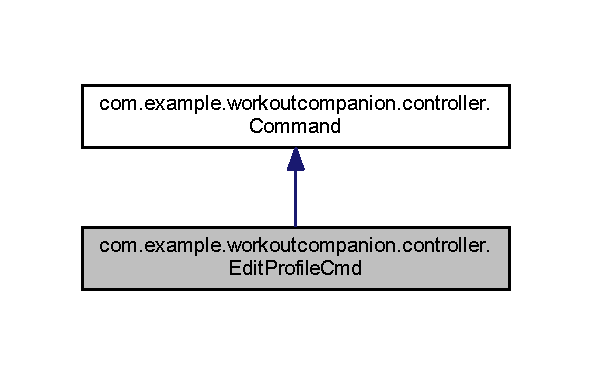
\includegraphics[width=284pt]{classcom_1_1example_1_1workoutcompanion_1_1controller_1_1_edit_profile_cmd__inherit__graph}
\end{center}
\end{figure}


Collaboration diagram for com.\-example.\-workoutcompanion.\-controller.\-Edit\-Profile\-Cmd\-:
\nopagebreak
\begin{figure}[H]
\begin{center}
\leavevmode
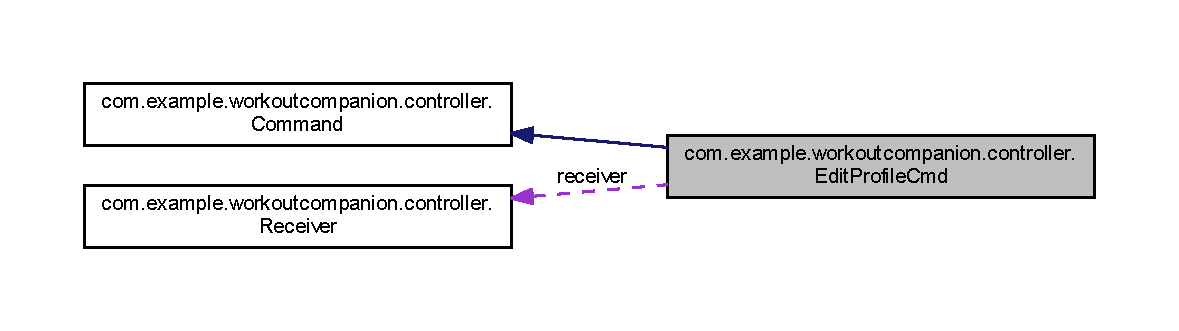
\includegraphics[width=350pt]{classcom_1_1example_1_1workoutcompanion_1_1controller_1_1_edit_profile_cmd__coll__graph}
\end{center}
\end{figure}
\subsection*{Public Member Functions}
\begin{DoxyCompactItemize}
\item 
\hyperlink{classcom_1_1example_1_1workoutcompanion_1_1controller_1_1_edit_profile_cmd_a602cc367fffbae2db5a420eb18ef72c8}{Edit\-Profile\-Cmd} (\hyperlink{classcom_1_1example_1_1workoutcompanion_1_1controller_1_1_receiver}{Receiver} receiver)
\item 
void \hyperlink{classcom_1_1example_1_1workoutcompanion_1_1controller_1_1_edit_profile_cmd_aa88c4baa3aa144886cfe457c8eb270ff}{execute} (String...\-names)
\end{DoxyCompactItemize}


\subsection{Constructor \& Destructor Documentation}
\hypertarget{classcom_1_1example_1_1workoutcompanion_1_1controller_1_1_edit_profile_cmd_a602cc367fffbae2db5a420eb18ef72c8}{\index{com\-::example\-::workoutcompanion\-::controller\-::\-Edit\-Profile\-Cmd@{com\-::example\-::workoutcompanion\-::controller\-::\-Edit\-Profile\-Cmd}!Edit\-Profile\-Cmd@{Edit\-Profile\-Cmd}}
\index{Edit\-Profile\-Cmd@{Edit\-Profile\-Cmd}!com::example::workoutcompanion::controller::EditProfileCmd@{com\-::example\-::workoutcompanion\-::controller\-::\-Edit\-Profile\-Cmd}}
\subsubsection[{Edit\-Profile\-Cmd}]{\setlength{\rightskip}{0pt plus 5cm}com.\-example.\-workoutcompanion.\-controller.\-Edit\-Profile\-Cmd.\-Edit\-Profile\-Cmd (
\begin{DoxyParamCaption}
\item[{{\bf Receiver}}]{receiver}
\end{DoxyParamCaption}
)}}\label{classcom_1_1example_1_1workoutcompanion_1_1controller_1_1_edit_profile_cmd_a602cc367fffbae2db5a420eb18ef72c8}


\subsection{Member Function Documentation}
\hypertarget{classcom_1_1example_1_1workoutcompanion_1_1controller_1_1_edit_profile_cmd_aa88c4baa3aa144886cfe457c8eb270ff}{\index{com\-::example\-::workoutcompanion\-::controller\-::\-Edit\-Profile\-Cmd@{com\-::example\-::workoutcompanion\-::controller\-::\-Edit\-Profile\-Cmd}!execute@{execute}}
\index{execute@{execute}!com::example::workoutcompanion::controller::EditProfileCmd@{com\-::example\-::workoutcompanion\-::controller\-::\-Edit\-Profile\-Cmd}}
\subsubsection[{execute}]{\setlength{\rightskip}{0pt plus 5cm}void com.\-example.\-workoutcompanion.\-controller.\-Edit\-Profile\-Cmd.\-execute (
\begin{DoxyParamCaption}
\item[{String...}]{names}
\end{DoxyParamCaption}
)}}\label{classcom_1_1example_1_1workoutcompanion_1_1controller_1_1_edit_profile_cmd_aa88c4baa3aa144886cfe457c8eb270ff}


Implements \hyperlink{interfacecom_1_1example_1_1workoutcompanion_1_1controller_1_1_command_ad947864c82a300557eed99dd8367c020}{com.\-example.\-workoutcompanion.\-controller.\-Command}.



The documentation for this class was generated from the following file\-:\begin{DoxyCompactItemize}
\item 
Desktop/git\-\_\-proj/workout/src/com/example/workoutcompanion/controller/\hyperlink{_edit_profile_cmd_8java}{Edit\-Profile\-Cmd.\-java}\end{DoxyCompactItemize}

\hypertarget{classcom_1_1example_1_1workoutcompanion_1_1controller_1_1_edit_workout_cmd}{\section{com.\-example.\-workoutcompanion.\-controller.\-Edit\-Workout\-Cmd Class Reference}
\label{classcom_1_1example_1_1workoutcompanion_1_1controller_1_1_edit_workout_cmd}\index{com.\-example.\-workoutcompanion.\-controller.\-Edit\-Workout\-Cmd@{com.\-example.\-workoutcompanion.\-controller.\-Edit\-Workout\-Cmd}}
}


Inheritance diagram for com.\-example.\-workoutcompanion.\-controller.\-Edit\-Workout\-Cmd\-:
\nopagebreak
\begin{figure}[H]
\begin{center}
\leavevmode
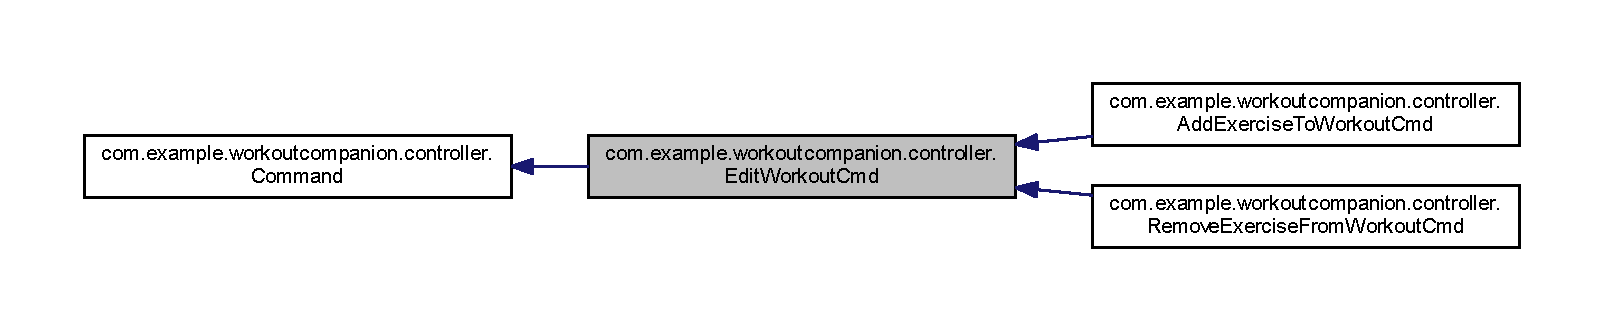
\includegraphics[width=350pt]{classcom_1_1example_1_1workoutcompanion_1_1controller_1_1_edit_workout_cmd__inherit__graph}
\end{center}
\end{figure}


Collaboration diagram for com.\-example.\-workoutcompanion.\-controller.\-Edit\-Workout\-Cmd\-:
\nopagebreak
\begin{figure}[H]
\begin{center}
\leavevmode
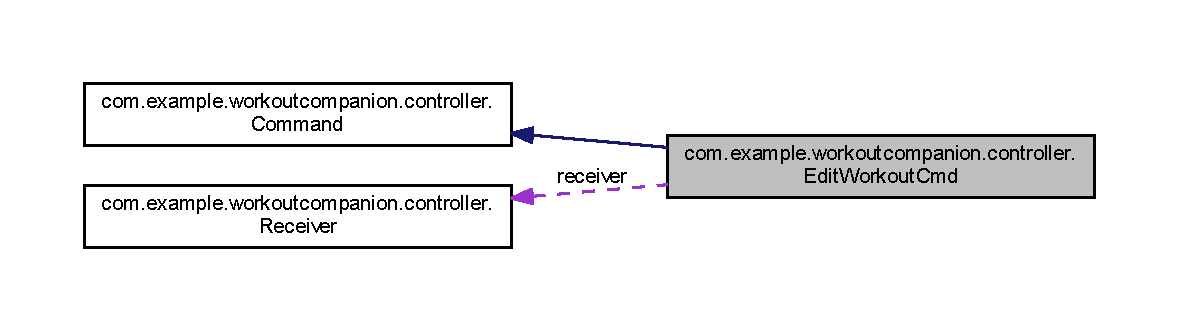
\includegraphics[width=350pt]{classcom_1_1example_1_1workoutcompanion_1_1controller_1_1_edit_workout_cmd__coll__graph}
\end{center}
\end{figure}
\subsection*{Public Member Functions}
\begin{DoxyCompactItemize}
\item 
\hyperlink{classcom_1_1example_1_1workoutcompanion_1_1controller_1_1_edit_workout_cmd_a8d6241f5081888e0bec1a15c8051e6ec}{Edit\-Workout\-Cmd} (\hyperlink{classcom_1_1example_1_1workoutcompanion_1_1controller_1_1_receiver}{Receiver} receiver)
\end{DoxyCompactItemize}


\subsection{Constructor \& Destructor Documentation}
\hypertarget{classcom_1_1example_1_1workoutcompanion_1_1controller_1_1_edit_workout_cmd_a8d6241f5081888e0bec1a15c8051e6ec}{\index{com\-::example\-::workoutcompanion\-::controller\-::\-Edit\-Workout\-Cmd@{com\-::example\-::workoutcompanion\-::controller\-::\-Edit\-Workout\-Cmd}!Edit\-Workout\-Cmd@{Edit\-Workout\-Cmd}}
\index{Edit\-Workout\-Cmd@{Edit\-Workout\-Cmd}!com::example::workoutcompanion::controller::EditWorkoutCmd@{com\-::example\-::workoutcompanion\-::controller\-::\-Edit\-Workout\-Cmd}}
\subsubsection[{Edit\-Workout\-Cmd}]{\setlength{\rightskip}{0pt plus 5cm}com.\-example.\-workoutcompanion.\-controller.\-Edit\-Workout\-Cmd.\-Edit\-Workout\-Cmd (
\begin{DoxyParamCaption}
\item[{{\bf Receiver}}]{receiver}
\end{DoxyParamCaption}
)}}\label{classcom_1_1example_1_1workoutcompanion_1_1controller_1_1_edit_workout_cmd_a8d6241f5081888e0bec1a15c8051e6ec}


The documentation for this class was generated from the following file\-:\begin{DoxyCompactItemize}
\item 
Desktop/git\-\_\-proj/workout/src/com/example/workoutcompanion/controller/\hyperlink{_edit_workout_cmd_8java}{Edit\-Workout\-Cmd.\-java}\end{DoxyCompactItemize}

\hypertarget{classcom_1_1example_1_1workoutcompanion_1_1dom_1_1_exercise}{\section{com.\-example.\-workoutcompanion.\-dom.\-Exercise Class Reference}
\label{classcom_1_1example_1_1workoutcompanion_1_1dom_1_1_exercise}\index{com.\-example.\-workoutcompanion.\-dom.\-Exercise@{com.\-example.\-workoutcompanion.\-dom.\-Exercise}}
}
\subsection*{Public Member Functions}
\begin{DoxyCompactItemize}
\item 
\hyperlink{classcom_1_1example_1_1workoutcompanion_1_1dom_1_1_exercise_a37072c8ae939cf4c97c09a6158eeafa6}{Exercise} (String a\-\_\-s\-Name)
\item 
Foreign\-Collection$<$ \hyperlink{classcom_1_1example_1_1workoutcompanion_1_1dom_1_1_workout}{Workout} $>$ \hyperlink{classcom_1_1example_1_1workoutcompanion_1_1dom_1_1_exercise_a7094714bc04027326cc8df11f3ca9386}{get\-Workouts} ()
\item 
String \hyperlink{classcom_1_1example_1_1workoutcompanion_1_1dom_1_1_exercise_aa3aa2d96310db78e6c78816929a80a9f}{get\-Name} ()
\item 
void \hyperlink{classcom_1_1example_1_1workoutcompanion_1_1dom_1_1_exercise_a3e169898ed772f62d20c2d2899c30eb6}{set\-Name} (String new\-Name)
\end{DoxyCompactItemize}
\subsection*{Static Public Attributes}
\begin{DoxyCompactItemize}
\item 
static final String \hyperlink{classcom_1_1example_1_1workoutcompanion_1_1dom_1_1_exercise_a1aeb9a6e42c38c3169197b37e8ee79f8}{E\-X\-E\-R\-C\-I\-S\-E\-\_\-\-N\-A\-M\-E\-\_\-\-C\-O\-L\-U\-M\-N\-\_\-\-F\-I\-E\-L\-D} = \char`\"{}name\char`\"{}
\end{DoxyCompactItemize}


\subsection{Constructor \& Destructor Documentation}
\hypertarget{classcom_1_1example_1_1workoutcompanion_1_1dom_1_1_exercise_a37072c8ae939cf4c97c09a6158eeafa6}{\index{com\-::example\-::workoutcompanion\-::dom\-::\-Exercise@{com\-::example\-::workoutcompanion\-::dom\-::\-Exercise}!Exercise@{Exercise}}
\index{Exercise@{Exercise}!com::example::workoutcompanion::dom::Exercise@{com\-::example\-::workoutcompanion\-::dom\-::\-Exercise}}
\subsubsection[{Exercise}]{\setlength{\rightskip}{0pt plus 5cm}com.\-example.\-workoutcompanion.\-dom.\-Exercise.\-Exercise (
\begin{DoxyParamCaption}
\item[{String}]{a\-\_\-s\-Name}
\end{DoxyParamCaption}
)}}\label{classcom_1_1example_1_1workoutcompanion_1_1dom_1_1_exercise_a37072c8ae939cf4c97c09a6158eeafa6}


\subsection{Member Function Documentation}
\hypertarget{classcom_1_1example_1_1workoutcompanion_1_1dom_1_1_exercise_aa3aa2d96310db78e6c78816929a80a9f}{\index{com\-::example\-::workoutcompanion\-::dom\-::\-Exercise@{com\-::example\-::workoutcompanion\-::dom\-::\-Exercise}!get\-Name@{get\-Name}}
\index{get\-Name@{get\-Name}!com::example::workoutcompanion::dom::Exercise@{com\-::example\-::workoutcompanion\-::dom\-::\-Exercise}}
\subsubsection[{get\-Name}]{\setlength{\rightskip}{0pt plus 5cm}String com.\-example.\-workoutcompanion.\-dom.\-Exercise.\-get\-Name (
\begin{DoxyParamCaption}
{}
\end{DoxyParamCaption}
)}}\label{classcom_1_1example_1_1workoutcompanion_1_1dom_1_1_exercise_aa3aa2d96310db78e6c78816929a80a9f}
\hypertarget{classcom_1_1example_1_1workoutcompanion_1_1dom_1_1_exercise_a7094714bc04027326cc8df11f3ca9386}{\index{com\-::example\-::workoutcompanion\-::dom\-::\-Exercise@{com\-::example\-::workoutcompanion\-::dom\-::\-Exercise}!get\-Workouts@{get\-Workouts}}
\index{get\-Workouts@{get\-Workouts}!com::example::workoutcompanion::dom::Exercise@{com\-::example\-::workoutcompanion\-::dom\-::\-Exercise}}
\subsubsection[{get\-Workouts}]{\setlength{\rightskip}{0pt plus 5cm}Foreign\-Collection$<${\bf Workout}$>$ com.\-example.\-workoutcompanion.\-dom.\-Exercise.\-get\-Workouts (
\begin{DoxyParamCaption}
{}
\end{DoxyParamCaption}
)}}\label{classcom_1_1example_1_1workoutcompanion_1_1dom_1_1_exercise_a7094714bc04027326cc8df11f3ca9386}
\hypertarget{classcom_1_1example_1_1workoutcompanion_1_1dom_1_1_exercise_a3e169898ed772f62d20c2d2899c30eb6}{\index{com\-::example\-::workoutcompanion\-::dom\-::\-Exercise@{com\-::example\-::workoutcompanion\-::dom\-::\-Exercise}!set\-Name@{set\-Name}}
\index{set\-Name@{set\-Name}!com::example::workoutcompanion::dom::Exercise@{com\-::example\-::workoutcompanion\-::dom\-::\-Exercise}}
\subsubsection[{set\-Name}]{\setlength{\rightskip}{0pt plus 5cm}void com.\-example.\-workoutcompanion.\-dom.\-Exercise.\-set\-Name (
\begin{DoxyParamCaption}
\item[{String}]{new\-Name}
\end{DoxyParamCaption}
)}}\label{classcom_1_1example_1_1workoutcompanion_1_1dom_1_1_exercise_a3e169898ed772f62d20c2d2899c30eb6}


\subsection{Member Data Documentation}
\hypertarget{classcom_1_1example_1_1workoutcompanion_1_1dom_1_1_exercise_a1aeb9a6e42c38c3169197b37e8ee79f8}{\index{com\-::example\-::workoutcompanion\-::dom\-::\-Exercise@{com\-::example\-::workoutcompanion\-::dom\-::\-Exercise}!E\-X\-E\-R\-C\-I\-S\-E\-\_\-\-N\-A\-M\-E\-\_\-\-C\-O\-L\-U\-M\-N\-\_\-\-F\-I\-E\-L\-D@{E\-X\-E\-R\-C\-I\-S\-E\-\_\-\-N\-A\-M\-E\-\_\-\-C\-O\-L\-U\-M\-N\-\_\-\-F\-I\-E\-L\-D}}
\index{E\-X\-E\-R\-C\-I\-S\-E\-\_\-\-N\-A\-M\-E\-\_\-\-C\-O\-L\-U\-M\-N\-\_\-\-F\-I\-E\-L\-D@{E\-X\-E\-R\-C\-I\-S\-E\-\_\-\-N\-A\-M\-E\-\_\-\-C\-O\-L\-U\-M\-N\-\_\-\-F\-I\-E\-L\-D}!com::example::workoutcompanion::dom::Exercise@{com\-::example\-::workoutcompanion\-::dom\-::\-Exercise}}
\subsubsection[{E\-X\-E\-R\-C\-I\-S\-E\-\_\-\-N\-A\-M\-E\-\_\-\-C\-O\-L\-U\-M\-N\-\_\-\-F\-I\-E\-L\-D}]{\setlength{\rightskip}{0pt plus 5cm}final String com.\-example.\-workoutcompanion.\-dom.\-Exercise.\-E\-X\-E\-R\-C\-I\-S\-E\-\_\-\-N\-A\-M\-E\-\_\-\-C\-O\-L\-U\-M\-N\-\_\-\-F\-I\-E\-L\-D = \char`\"{}name\char`\"{}\hspace{0.3cm}{\ttfamily [static]}}}\label{classcom_1_1example_1_1workoutcompanion_1_1dom_1_1_exercise_a1aeb9a6e42c38c3169197b37e8ee79f8}


The documentation for this class was generated from the following file\-:\begin{DoxyCompactItemize}
\item 
Desktop/git\-\_\-proj/workout/src/com/example/workoutcompanion/dom/\hyperlink{_exercise_8java}{Exercise.\-java}\end{DoxyCompactItemize}

\hypertarget{classcom_1_1example_1_1workoutcompanion_1_1dom_1_1_profile}{\section{com.\-example.\-workoutcompanion.\-dom.\-Profile Class Reference}
\label{classcom_1_1example_1_1workoutcompanion_1_1dom_1_1_profile}\index{com.\-example.\-workoutcompanion.\-dom.\-Profile@{com.\-example.\-workoutcompanion.\-dom.\-Profile}}
}
\subsection*{Public Member Functions}
\begin{DoxyCompactItemize}
\item 
\hyperlink{classcom_1_1example_1_1workoutcompanion_1_1dom_1_1_profile_a7864d394beb2f58cca1319c57d525048}{Profile} ()
\item 
void \hyperlink{classcom_1_1example_1_1workoutcompanion_1_1dom_1_1_profile_ab7f72d54e1eb8cf4311e025ad4629a01}{add\-Workout} (\hyperlink{classcom_1_1example_1_1workoutcompanion_1_1dom_1_1_workout}{Workout} workout)
\item 
void \hyperlink{classcom_1_1example_1_1workoutcompanion_1_1dom_1_1_profile_a7bc92d322add1308cba46dafd1018195}{remove\-Workout} (\hyperlink{classcom_1_1example_1_1workoutcompanion_1_1dom_1_1_workout}{Workout} workout)
\item 
String \hyperlink{classcom_1_1example_1_1workoutcompanion_1_1dom_1_1_profile_a226ddee02ad02b0dd027f754dede5031}{get\-Name} ()
\item 
void \hyperlink{classcom_1_1example_1_1workoutcompanion_1_1dom_1_1_profile_a127e4507e0f6c9eb08125a1507a01944}{set\-Name} (String name)
\item 
List$<$ \hyperlink{classcom_1_1example_1_1workoutcompanion_1_1dom_1_1_workout}{Workout} $>$ \hyperlink{classcom_1_1example_1_1workoutcompanion_1_1dom_1_1_profile_af184b95d5481b6bc850b602b470a02c1}{get\-Workouts} ()
\item 
void \hyperlink{classcom_1_1example_1_1workoutcompanion_1_1dom_1_1_profile_a33221af697e6082f614da117a87a28a1}{set\-Workouts} (List$<$ \hyperlink{classcom_1_1example_1_1workoutcompanion_1_1dom_1_1_workout}{Workout} $>$ workouts)
\end{DoxyCompactItemize}


\subsection{Constructor \& Destructor Documentation}
\hypertarget{classcom_1_1example_1_1workoutcompanion_1_1dom_1_1_profile_a7864d394beb2f58cca1319c57d525048}{\index{com\-::example\-::workoutcompanion\-::dom\-::\-Profile@{com\-::example\-::workoutcompanion\-::dom\-::\-Profile}!Profile@{Profile}}
\index{Profile@{Profile}!com::example::workoutcompanion::dom::Profile@{com\-::example\-::workoutcompanion\-::dom\-::\-Profile}}
\subsubsection[{Profile}]{\setlength{\rightskip}{0pt plus 5cm}com.\-example.\-workoutcompanion.\-dom.\-Profile.\-Profile (
\begin{DoxyParamCaption}
{}
\end{DoxyParamCaption}
)}}\label{classcom_1_1example_1_1workoutcompanion_1_1dom_1_1_profile_a7864d394beb2f58cca1319c57d525048}


\subsection{Member Function Documentation}
\hypertarget{classcom_1_1example_1_1workoutcompanion_1_1dom_1_1_profile_ab7f72d54e1eb8cf4311e025ad4629a01}{\index{com\-::example\-::workoutcompanion\-::dom\-::\-Profile@{com\-::example\-::workoutcompanion\-::dom\-::\-Profile}!add\-Workout@{add\-Workout}}
\index{add\-Workout@{add\-Workout}!com::example::workoutcompanion::dom::Profile@{com\-::example\-::workoutcompanion\-::dom\-::\-Profile}}
\subsubsection[{add\-Workout}]{\setlength{\rightskip}{0pt plus 5cm}void com.\-example.\-workoutcompanion.\-dom.\-Profile.\-add\-Workout (
\begin{DoxyParamCaption}
\item[{{\bf Workout}}]{workout}
\end{DoxyParamCaption}
)}}\label{classcom_1_1example_1_1workoutcompanion_1_1dom_1_1_profile_ab7f72d54e1eb8cf4311e025ad4629a01}
\hypertarget{classcom_1_1example_1_1workoutcompanion_1_1dom_1_1_profile_a226ddee02ad02b0dd027f754dede5031}{\index{com\-::example\-::workoutcompanion\-::dom\-::\-Profile@{com\-::example\-::workoutcompanion\-::dom\-::\-Profile}!get\-Name@{get\-Name}}
\index{get\-Name@{get\-Name}!com::example::workoutcompanion::dom::Profile@{com\-::example\-::workoutcompanion\-::dom\-::\-Profile}}
\subsubsection[{get\-Name}]{\setlength{\rightskip}{0pt plus 5cm}String com.\-example.\-workoutcompanion.\-dom.\-Profile.\-get\-Name (
\begin{DoxyParamCaption}
{}
\end{DoxyParamCaption}
)}}\label{classcom_1_1example_1_1workoutcompanion_1_1dom_1_1_profile_a226ddee02ad02b0dd027f754dede5031}
\hypertarget{classcom_1_1example_1_1workoutcompanion_1_1dom_1_1_profile_af184b95d5481b6bc850b602b470a02c1}{\index{com\-::example\-::workoutcompanion\-::dom\-::\-Profile@{com\-::example\-::workoutcompanion\-::dom\-::\-Profile}!get\-Workouts@{get\-Workouts}}
\index{get\-Workouts@{get\-Workouts}!com::example::workoutcompanion::dom::Profile@{com\-::example\-::workoutcompanion\-::dom\-::\-Profile}}
\subsubsection[{get\-Workouts}]{\setlength{\rightskip}{0pt plus 5cm}List$<${\bf Workout}$>$ com.\-example.\-workoutcompanion.\-dom.\-Profile.\-get\-Workouts (
\begin{DoxyParamCaption}
{}
\end{DoxyParamCaption}
)}}\label{classcom_1_1example_1_1workoutcompanion_1_1dom_1_1_profile_af184b95d5481b6bc850b602b470a02c1}
\hypertarget{classcom_1_1example_1_1workoutcompanion_1_1dom_1_1_profile_a7bc92d322add1308cba46dafd1018195}{\index{com\-::example\-::workoutcompanion\-::dom\-::\-Profile@{com\-::example\-::workoutcompanion\-::dom\-::\-Profile}!remove\-Workout@{remove\-Workout}}
\index{remove\-Workout@{remove\-Workout}!com::example::workoutcompanion::dom::Profile@{com\-::example\-::workoutcompanion\-::dom\-::\-Profile}}
\subsubsection[{remove\-Workout}]{\setlength{\rightskip}{0pt plus 5cm}void com.\-example.\-workoutcompanion.\-dom.\-Profile.\-remove\-Workout (
\begin{DoxyParamCaption}
\item[{{\bf Workout}}]{workout}
\end{DoxyParamCaption}
)}}\label{classcom_1_1example_1_1workoutcompanion_1_1dom_1_1_profile_a7bc92d322add1308cba46dafd1018195}
\hypertarget{classcom_1_1example_1_1workoutcompanion_1_1dom_1_1_profile_a127e4507e0f6c9eb08125a1507a01944}{\index{com\-::example\-::workoutcompanion\-::dom\-::\-Profile@{com\-::example\-::workoutcompanion\-::dom\-::\-Profile}!set\-Name@{set\-Name}}
\index{set\-Name@{set\-Name}!com::example::workoutcompanion::dom::Profile@{com\-::example\-::workoutcompanion\-::dom\-::\-Profile}}
\subsubsection[{set\-Name}]{\setlength{\rightskip}{0pt plus 5cm}void com.\-example.\-workoutcompanion.\-dom.\-Profile.\-set\-Name (
\begin{DoxyParamCaption}
\item[{String}]{name}
\end{DoxyParamCaption}
)}}\label{classcom_1_1example_1_1workoutcompanion_1_1dom_1_1_profile_a127e4507e0f6c9eb08125a1507a01944}
\hypertarget{classcom_1_1example_1_1workoutcompanion_1_1dom_1_1_profile_a33221af697e6082f614da117a87a28a1}{\index{com\-::example\-::workoutcompanion\-::dom\-::\-Profile@{com\-::example\-::workoutcompanion\-::dom\-::\-Profile}!set\-Workouts@{set\-Workouts}}
\index{set\-Workouts@{set\-Workouts}!com::example::workoutcompanion::dom::Profile@{com\-::example\-::workoutcompanion\-::dom\-::\-Profile}}
\subsubsection[{set\-Workouts}]{\setlength{\rightskip}{0pt plus 5cm}void com.\-example.\-workoutcompanion.\-dom.\-Profile.\-set\-Workouts (
\begin{DoxyParamCaption}
\item[{List$<$ {\bf Workout} $>$}]{workouts}
\end{DoxyParamCaption}
)}}\label{classcom_1_1example_1_1workoutcompanion_1_1dom_1_1_profile_a33221af697e6082f614da117a87a28a1}


The documentation for this class was generated from the following file\-:\begin{DoxyCompactItemize}
\item 
Desktop/git\-\_\-proj/workout/src/com/example/workoutcompanion/dom/\hyperlink{_profile_8java}{Profile.\-java}\end{DoxyCompactItemize}

\hypertarget{classcom_1_1example_1_1workoutcompanion_1_1_profile_fragment}{\section{com.\-example.\-workoutcompanion.\-Profile\-Fragment Class Reference}
\label{classcom_1_1example_1_1workoutcompanion_1_1_profile_fragment}\index{com.\-example.\-workoutcompanion.\-Profile\-Fragment@{com.\-example.\-workoutcompanion.\-Profile\-Fragment}}
}


Inheritance diagram for com.\-example.\-workoutcompanion.\-Profile\-Fragment\-:
\nopagebreak
\begin{figure}[H]
\begin{center}
\leavevmode
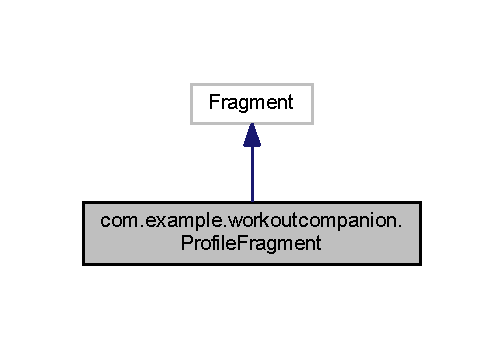
\includegraphics[width=242pt]{classcom_1_1example_1_1workoutcompanion_1_1_profile_fragment__inherit__graph}
\end{center}
\end{figure}


Collaboration diagram for com.\-example.\-workoutcompanion.\-Profile\-Fragment\-:
\nopagebreak
\begin{figure}[H]
\begin{center}
\leavevmode
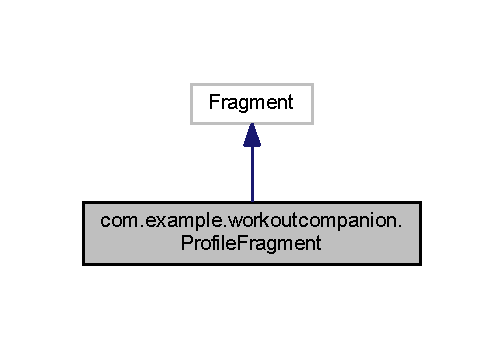
\includegraphics[width=242pt]{classcom_1_1example_1_1workoutcompanion_1_1_profile_fragment__coll__graph}
\end{center}
\end{figure}
\subsection*{Public Member Functions}
\begin{DoxyCompactItemize}
\item 
\hyperlink{classcom_1_1example_1_1workoutcompanion_1_1_profile_fragment_a85723fbb871783d0e1d7815a512f38a8}{Profile\-Fragment} ()
\item 
View \hyperlink{classcom_1_1example_1_1workoutcompanion_1_1_profile_fragment_a0593966558a1be66ac1bca16dc2da213}{on\-Create\-View} (final Layout\-Inflater inflater, final View\-Group container, Bundle saved\-Instance\-State)
\end{DoxyCompactItemize}


\subsection{Constructor \& Destructor Documentation}
\hypertarget{classcom_1_1example_1_1workoutcompanion_1_1_profile_fragment_a85723fbb871783d0e1d7815a512f38a8}{\index{com\-::example\-::workoutcompanion\-::\-Profile\-Fragment@{com\-::example\-::workoutcompanion\-::\-Profile\-Fragment}!Profile\-Fragment@{Profile\-Fragment}}
\index{Profile\-Fragment@{Profile\-Fragment}!com::example::workoutcompanion::ProfileFragment@{com\-::example\-::workoutcompanion\-::\-Profile\-Fragment}}
\subsubsection[{Profile\-Fragment}]{\setlength{\rightskip}{0pt plus 5cm}com.\-example.\-workoutcompanion.\-Profile\-Fragment.\-Profile\-Fragment (
\begin{DoxyParamCaption}
{}
\end{DoxyParamCaption}
)}}\label{classcom_1_1example_1_1workoutcompanion_1_1_profile_fragment_a85723fbb871783d0e1d7815a512f38a8}


\subsection{Member Function Documentation}
\hypertarget{classcom_1_1example_1_1workoutcompanion_1_1_profile_fragment_a0593966558a1be66ac1bca16dc2da213}{\index{com\-::example\-::workoutcompanion\-::\-Profile\-Fragment@{com\-::example\-::workoutcompanion\-::\-Profile\-Fragment}!on\-Create\-View@{on\-Create\-View}}
\index{on\-Create\-View@{on\-Create\-View}!com::example::workoutcompanion::ProfileFragment@{com\-::example\-::workoutcompanion\-::\-Profile\-Fragment}}
\subsubsection[{on\-Create\-View}]{\setlength{\rightskip}{0pt plus 5cm}View com.\-example.\-workoutcompanion.\-Profile\-Fragment.\-on\-Create\-View (
\begin{DoxyParamCaption}
\item[{final Layout\-Inflater}]{inflater, }
\item[{final View\-Group}]{container, }
\item[{Bundle}]{saved\-Instance\-State}
\end{DoxyParamCaption}
)}}\label{classcom_1_1example_1_1workoutcompanion_1_1_profile_fragment_a0593966558a1be66ac1bca16dc2da213}


The documentation for this class was generated from the following file\-:\begin{DoxyCompactItemize}
\item 
Desktop/git\-\_\-proj/workout/src/com/example/workoutcompanion/\hyperlink{_profile_fragment_8java}{Profile\-Fragment.\-java}\end{DoxyCompactItemize}

\hypertarget{classcom_1_1example_1_1workoutcompanion_1_1_r}{\section{com.\-example.\-workoutcompanion.\-R Class Reference}
\label{classcom_1_1example_1_1workoutcompanion_1_1_r}\index{com.\-example.\-workoutcompanion.\-R@{com.\-example.\-workoutcompanion.\-R}}
}
\subsection*{Classes}
\begin{DoxyCompactItemize}
\item 
class {\bfseries attr}
\item 
class {\bfseries dimen}
\item 
class {\bfseries drawable}
\item 
class {\bfseries id}
\item 
class {\bfseries layout}
\item 
class {\bfseries menu}
\item 
class {\bfseries string}
\item 
class {\bfseries style}
\end{DoxyCompactItemize}


The documentation for this class was generated from the following file\-:\begin{DoxyCompactItemize}
\item 
Desktop/git\-\_\-proj/workout/gen/com/example/workoutcompanion/\hyperlink{_r_8java}{R.\-java}\end{DoxyCompactItemize}

\hypertarget{classcom_1_1example_1_1workoutcompanion_1_1controller_1_1_receiver}{\section{com.\-example.\-workoutcompanion.\-controller.\-Receiver Class Reference}
\label{classcom_1_1example_1_1workoutcompanion_1_1controller_1_1_receiver}\index{com.\-example.\-workoutcompanion.\-controller.\-Receiver@{com.\-example.\-workoutcompanion.\-controller.\-Receiver}}
}
\subsection*{Public Member Functions}
\begin{DoxyCompactItemize}
\item 
\hyperlink{classcom_1_1example_1_1workoutcompanion_1_1controller_1_1_receiver_acfb96b1541e3ba23321ed2d48cbbead1}{Receiver} (Context context)
\item 
boolean \hyperlink{classcom_1_1example_1_1workoutcompanion_1_1controller_1_1_receiver_a4dcbb836cd0af78eb9ff1960b06fffcb}{Create\-Workout} (String workout\-Name, String\mbox{[}$\,$\mbox{]} exercises)
\item 
boolean \hyperlink{classcom_1_1example_1_1workoutcompanion_1_1controller_1_1_receiver_a4a001b8158e4f00285c3a1c0302349f5}{Edit\-Workout} (String workout\-Name, String\mbox{[}$\,$\mbox{]} ex\-To\-Add, String\mbox{[}$\,$\mbox{]} ex\-To\-Rem)
\item 
boolean \hyperlink{classcom_1_1example_1_1workoutcompanion_1_1controller_1_1_receiver_a96eb1deda2a7bd7278c42df823a520f4}{Create\-Exercise} (String exercise\-Name)
\item 
boolean \hyperlink{classcom_1_1example_1_1workoutcompanion_1_1controller_1_1_receiver_af5807c400c5c805c8807d7bacd138c0b}{Edit\-Exercise} (String exercise\-Name)
\item 
boolean \hyperlink{classcom_1_1example_1_1workoutcompanion_1_1controller_1_1_receiver_a8cc04e91e624349f214b4550ab61ce56}{Edit\-Profile} ()
\end{DoxyCompactItemize}


\subsection{Constructor \& Destructor Documentation}
\hypertarget{classcom_1_1example_1_1workoutcompanion_1_1controller_1_1_receiver_acfb96b1541e3ba23321ed2d48cbbead1}{\index{com\-::example\-::workoutcompanion\-::controller\-::\-Receiver@{com\-::example\-::workoutcompanion\-::controller\-::\-Receiver}!Receiver@{Receiver}}
\index{Receiver@{Receiver}!com::example::workoutcompanion::controller::Receiver@{com\-::example\-::workoutcompanion\-::controller\-::\-Receiver}}
\subsubsection[{Receiver}]{\setlength{\rightskip}{0pt plus 5cm}com.\-example.\-workoutcompanion.\-controller.\-Receiver.\-Receiver (
\begin{DoxyParamCaption}
\item[{Context}]{context}
\end{DoxyParamCaption}
)}}\label{classcom_1_1example_1_1workoutcompanion_1_1controller_1_1_receiver_acfb96b1541e3ba23321ed2d48cbbead1}
Constructor for receiver. Creates Database\-Handler based on supplied context. 
\begin{DoxyParams}{Parameters}
{\em context} & Some context \\
\hline
\end{DoxyParams}


\subsection{Member Function Documentation}
\hypertarget{classcom_1_1example_1_1workoutcompanion_1_1controller_1_1_receiver_a96eb1deda2a7bd7278c42df823a520f4}{\index{com\-::example\-::workoutcompanion\-::controller\-::\-Receiver@{com\-::example\-::workoutcompanion\-::controller\-::\-Receiver}!Create\-Exercise@{Create\-Exercise}}
\index{Create\-Exercise@{Create\-Exercise}!com::example::workoutcompanion::controller::Receiver@{com\-::example\-::workoutcompanion\-::controller\-::\-Receiver}}
\subsubsection[{Create\-Exercise}]{\setlength{\rightskip}{0pt plus 5cm}boolean com.\-example.\-workoutcompanion.\-controller.\-Receiver.\-Create\-Exercise (
\begin{DoxyParamCaption}
\item[{String}]{exercise\-Name}
\end{DoxyParamCaption}
)}}\label{classcom_1_1example_1_1workoutcompanion_1_1controller_1_1_receiver_a96eb1deda2a7bd7278c42df823a520f4}
Creates an exercise for the given name. 
\begin{DoxyParams}{Parameters}
{\em exercise\-Name} & String Name of the exercise \\
\hline
\end{DoxyParams}
\begin{DoxyReturn}{Returns}
boolean success 
\end{DoxyReturn}
\hypertarget{classcom_1_1example_1_1workoutcompanion_1_1controller_1_1_receiver_a4dcbb836cd0af78eb9ff1960b06fffcb}{\index{com\-::example\-::workoutcompanion\-::controller\-::\-Receiver@{com\-::example\-::workoutcompanion\-::controller\-::\-Receiver}!Create\-Workout@{Create\-Workout}}
\index{Create\-Workout@{Create\-Workout}!com::example::workoutcompanion::controller::Receiver@{com\-::example\-::workoutcompanion\-::controller\-::\-Receiver}}
\subsubsection[{Create\-Workout}]{\setlength{\rightskip}{0pt plus 5cm}boolean com.\-example.\-workoutcompanion.\-controller.\-Receiver.\-Create\-Workout (
\begin{DoxyParamCaption}
\item[{String}]{workout\-Name, }
\item[{String\mbox{[}$\,$\mbox{]}}]{exercises}
\end{DoxyParamCaption}
)}}\label{classcom_1_1example_1_1workoutcompanion_1_1controller_1_1_receiver_a4dcbb836cd0af78eb9ff1960b06fffcb}
Creates workout for given string name and array of string exercises. 
\begin{DoxyParams}{Parameters}
{\em workout\-Name} & String Name of workout \\
\hline
{\em exercises} & String\mbox{[}\mbox{]} Array of exercise names \\
\hline
\end{DoxyParams}
\begin{DoxyReturn}{Returns}
boolean success 
\end{DoxyReturn}
\hypertarget{classcom_1_1example_1_1workoutcompanion_1_1controller_1_1_receiver_af5807c400c5c805c8807d7bacd138c0b}{\index{com\-::example\-::workoutcompanion\-::controller\-::\-Receiver@{com\-::example\-::workoutcompanion\-::controller\-::\-Receiver}!Edit\-Exercise@{Edit\-Exercise}}
\index{Edit\-Exercise@{Edit\-Exercise}!com::example::workoutcompanion::controller::Receiver@{com\-::example\-::workoutcompanion\-::controller\-::\-Receiver}}
\subsubsection[{Edit\-Exercise}]{\setlength{\rightskip}{0pt plus 5cm}boolean com.\-example.\-workoutcompanion.\-controller.\-Receiver.\-Edit\-Exercise (
\begin{DoxyParamCaption}
\item[{String}]{exercise\-Name}
\end{DoxyParamCaption}
)}}\label{classcom_1_1example_1_1workoutcompanion_1_1controller_1_1_receiver_af5807c400c5c805c8807d7bacd138c0b}
Edits an exercise that is present in the database. 
\begin{DoxyParams}{Parameters}
{\em exercise\-Name} & String Name of exercise \\
\hline
\end{DoxyParams}
\begin{DoxyReturn}{Returns}
boolean success 
\end{DoxyReturn}
\hypertarget{classcom_1_1example_1_1workoutcompanion_1_1controller_1_1_receiver_a8cc04e91e624349f214b4550ab61ce56}{\index{com\-::example\-::workoutcompanion\-::controller\-::\-Receiver@{com\-::example\-::workoutcompanion\-::controller\-::\-Receiver}!Edit\-Profile@{Edit\-Profile}}
\index{Edit\-Profile@{Edit\-Profile}!com::example::workoutcompanion::controller::Receiver@{com\-::example\-::workoutcompanion\-::controller\-::\-Receiver}}
\subsubsection[{Edit\-Profile}]{\setlength{\rightskip}{0pt plus 5cm}boolean com.\-example.\-workoutcompanion.\-controller.\-Receiver.\-Edit\-Profile (
\begin{DoxyParamCaption}
{}
\end{DoxyParamCaption}
)}}\label{classcom_1_1example_1_1workoutcompanion_1_1controller_1_1_receiver_a8cc04e91e624349f214b4550ab61ce56}
\begin{DoxyReturn}{Returns}

\end{DoxyReturn}
\hypertarget{classcom_1_1example_1_1workoutcompanion_1_1controller_1_1_receiver_a4a001b8158e4f00285c3a1c0302349f5}{\index{com\-::example\-::workoutcompanion\-::controller\-::\-Receiver@{com\-::example\-::workoutcompanion\-::controller\-::\-Receiver}!Edit\-Workout@{Edit\-Workout}}
\index{Edit\-Workout@{Edit\-Workout}!com::example::workoutcompanion::controller::Receiver@{com\-::example\-::workoutcompanion\-::controller\-::\-Receiver}}
\subsubsection[{Edit\-Workout}]{\setlength{\rightskip}{0pt plus 5cm}boolean com.\-example.\-workoutcompanion.\-controller.\-Receiver.\-Edit\-Workout (
\begin{DoxyParamCaption}
\item[{String}]{workout\-Name, }
\item[{String\mbox{[}$\,$\mbox{]}}]{ex\-To\-Add, }
\item[{String\mbox{[}$\,$\mbox{]}}]{ex\-To\-Rem}
\end{DoxyParamCaption}
)}}\label{classcom_1_1example_1_1workoutcompanion_1_1controller_1_1_receiver_a4a001b8158e4f00285c3a1c0302349f5}
Edits the database entry for given workout to hold new exercises 
\begin{DoxyParams}{Parameters}
{\em workout\-Name} & String Name of workout to edit \\
\hline
{\em ex\-To\-Add} & String\mbox{[}\mbox{]} Names of exercises to add to workout \\
\hline
{\em ex\-To\-Rem} & String\mbox{[}\mbox{]} Names of exercises to remove from workout \\
\hline
\end{DoxyParams}
\begin{DoxyReturn}{Returns}
boolean success 
\end{DoxyReturn}


The documentation for this class was generated from the following file\-:\begin{DoxyCompactItemize}
\item 
Desktop/git\-\_\-proj/workout/src/com/example/workoutcompanion/controller/\hyperlink{_receiver_8java}{Receiver.\-java}\end{DoxyCompactItemize}

\hypertarget{classcom_1_1example_1_1workoutcompanion_1_1controller_1_1_remove_exercise_from_workout_cmd}{\section{com.\-example.\-workoutcompanion.\-controller.\-Remove\-Exercise\-From\-Workout\-Cmd Class Reference}
\label{classcom_1_1example_1_1workoutcompanion_1_1controller_1_1_remove_exercise_from_workout_cmd}\index{com.\-example.\-workoutcompanion.\-controller.\-Remove\-Exercise\-From\-Workout\-Cmd@{com.\-example.\-workoutcompanion.\-controller.\-Remove\-Exercise\-From\-Workout\-Cmd}}
}


Inheritance diagram for com.\-example.\-workoutcompanion.\-controller.\-Remove\-Exercise\-From\-Workout\-Cmd\-:\nopagebreak
\begin{figure}[H]
\begin{center}
\leavevmode
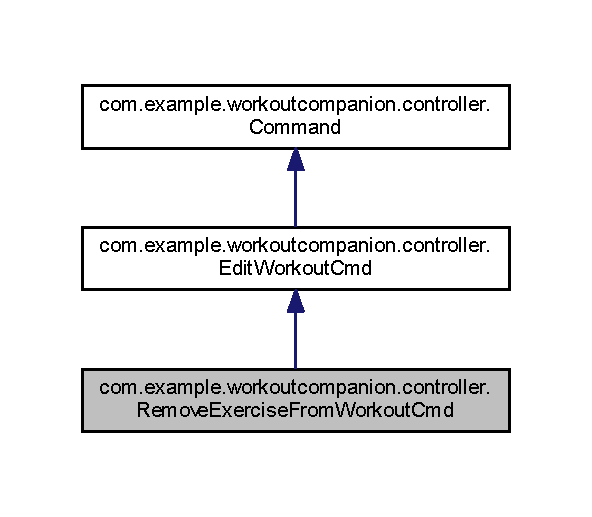
\includegraphics[width=284pt]{classcom_1_1example_1_1workoutcompanion_1_1controller_1_1_remove_exercise_from_workout_cmd__inherit__graph}
\end{center}
\end{figure}


Collaboration diagram for com.\-example.\-workoutcompanion.\-controller.\-Remove\-Exercise\-From\-Workout\-Cmd\-:\nopagebreak
\begin{figure}[H]
\begin{center}
\leavevmode
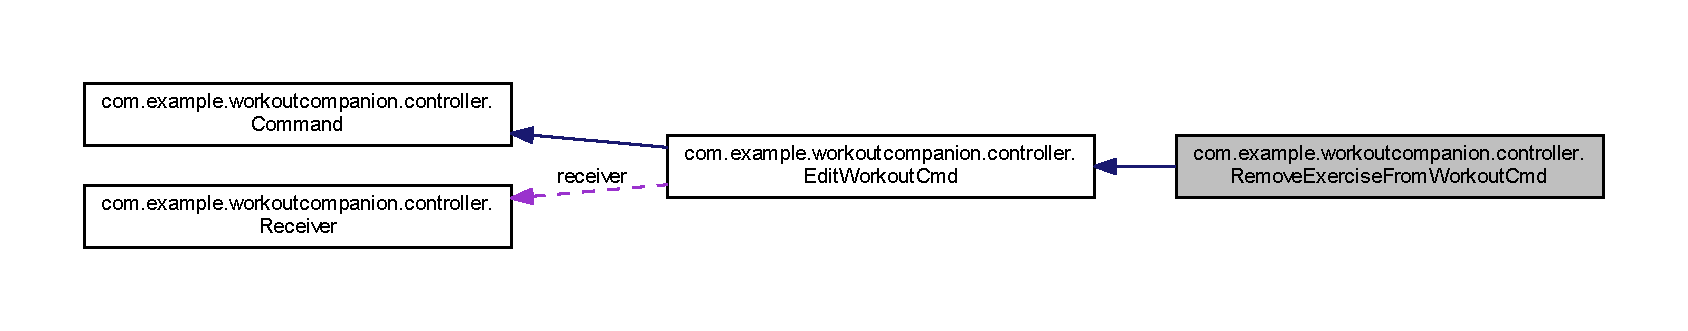
\includegraphics[width=350pt]{classcom_1_1example_1_1workoutcompanion_1_1controller_1_1_remove_exercise_from_workout_cmd__coll__graph}
\end{center}
\end{figure}
\subsection*{Public Member Functions}
\begin{DoxyCompactItemize}
\item 
\hyperlink{classcom_1_1example_1_1workoutcompanion_1_1controller_1_1_remove_exercise_from_workout_cmd_aabaca203f29f355d4e40b757f2b58032}{Remove\-Exercise\-From\-Workout\-Cmd} (\hyperlink{classcom_1_1example_1_1workoutcompanion_1_1controller_1_1_receiver}{Receiver} receiver)
\item 
void \hyperlink{classcom_1_1example_1_1workoutcompanion_1_1controller_1_1_remove_exercise_from_workout_cmd_aa1212feda70af3ae8eb41f2a47fc38e8}{execute} (String...\-names)
\end{DoxyCompactItemize}


\subsection{Constructor \& Destructor Documentation}
\hypertarget{classcom_1_1example_1_1workoutcompanion_1_1controller_1_1_remove_exercise_from_workout_cmd_aabaca203f29f355d4e40b757f2b58032}{\index{com\-::example\-::workoutcompanion\-::controller\-::\-Remove\-Exercise\-From\-Workout\-Cmd@{com\-::example\-::workoutcompanion\-::controller\-::\-Remove\-Exercise\-From\-Workout\-Cmd}!Remove\-Exercise\-From\-Workout\-Cmd@{Remove\-Exercise\-From\-Workout\-Cmd}}
\index{Remove\-Exercise\-From\-Workout\-Cmd@{Remove\-Exercise\-From\-Workout\-Cmd}!com::example::workoutcompanion::controller::RemoveExerciseFromWorkoutCmd@{com\-::example\-::workoutcompanion\-::controller\-::\-Remove\-Exercise\-From\-Workout\-Cmd}}
\subsubsection[{Remove\-Exercise\-From\-Workout\-Cmd}]{\setlength{\rightskip}{0pt plus 5cm}com.\-example.\-workoutcompanion.\-controller.\-Remove\-Exercise\-From\-Workout\-Cmd.\-Remove\-Exercise\-From\-Workout\-Cmd (
\begin{DoxyParamCaption}
\item[{{\bf Receiver}}]{receiver}
\end{DoxyParamCaption}
)}}\label{classcom_1_1example_1_1workoutcompanion_1_1controller_1_1_remove_exercise_from_workout_cmd_aabaca203f29f355d4e40b757f2b58032}


\subsection{Member Function Documentation}
\hypertarget{classcom_1_1example_1_1workoutcompanion_1_1controller_1_1_remove_exercise_from_workout_cmd_aa1212feda70af3ae8eb41f2a47fc38e8}{\index{com\-::example\-::workoutcompanion\-::controller\-::\-Remove\-Exercise\-From\-Workout\-Cmd@{com\-::example\-::workoutcompanion\-::controller\-::\-Remove\-Exercise\-From\-Workout\-Cmd}!execute@{execute}}
\index{execute@{execute}!com::example::workoutcompanion::controller::RemoveExerciseFromWorkoutCmd@{com\-::example\-::workoutcompanion\-::controller\-::\-Remove\-Exercise\-From\-Workout\-Cmd}}
\subsubsection[{execute}]{\setlength{\rightskip}{0pt plus 5cm}void com.\-example.\-workoutcompanion.\-controller.\-Remove\-Exercise\-From\-Workout\-Cmd.\-execute (
\begin{DoxyParamCaption}
\item[{String...}]{names}
\end{DoxyParamCaption}
)}}\label{classcom_1_1example_1_1workoutcompanion_1_1controller_1_1_remove_exercise_from_workout_cmd_aa1212feda70af3ae8eb41f2a47fc38e8}


Implements \hyperlink{interfacecom_1_1example_1_1workoutcompanion_1_1controller_1_1_command_ad947864c82a300557eed99dd8367c020}{com.\-example.\-workoutcompanion.\-controller.\-Command}.



The documentation for this class was generated from the following file\-:\begin{DoxyCompactItemize}
\item 
Desktop/git\-\_\-proj/workout/src/com/example/workoutcompanion/controller/\hyperlink{_remove_exercise_from_workout_cmd_8java}{Remove\-Exercise\-From\-Workout\-Cmd.\-java}\end{DoxyCompactItemize}

\hypertarget{classcom_1_1example_1_1workoutcompanion_1_1_workout_activity_1_1_sections_pager_adapter}{\section{com.\-example.\-workoutcompanion.\-Workout\-Activity.\-Sections\-Pager\-Adapter Class Reference}
\label{classcom_1_1example_1_1workoutcompanion_1_1_workout_activity_1_1_sections_pager_adapter}\index{com.\-example.\-workoutcompanion.\-Workout\-Activity.\-Sections\-Pager\-Adapter@{com.\-example.\-workoutcompanion.\-Workout\-Activity.\-Sections\-Pager\-Adapter}}
}


Inheritance diagram for com.\-example.\-workoutcompanion.\-Workout\-Activity.\-Sections\-Pager\-Adapter\-:
\nopagebreak
\begin{figure}[H]
\begin{center}
\leavevmode
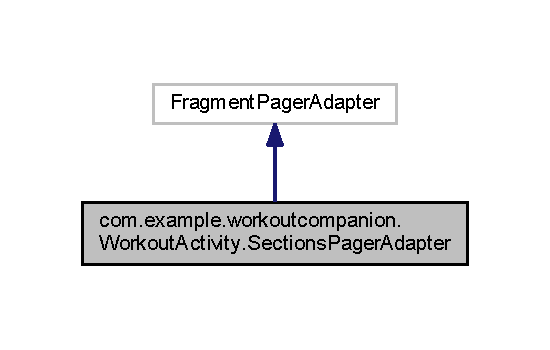
\includegraphics[width=264pt]{classcom_1_1example_1_1workoutcompanion_1_1_workout_activity_1_1_sections_pager_adapter__inherit__graph}
\end{center}
\end{figure}


Collaboration diagram for com.\-example.\-workoutcompanion.\-Workout\-Activity.\-Sections\-Pager\-Adapter\-:
\nopagebreak
\begin{figure}[H]
\begin{center}
\leavevmode
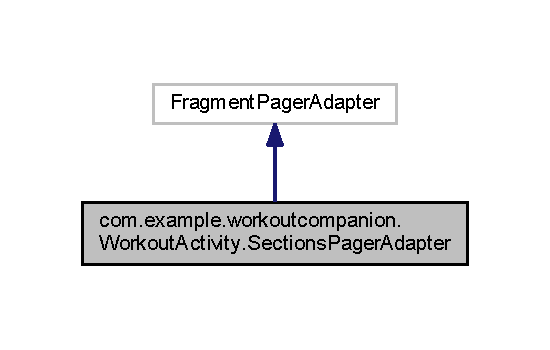
\includegraphics[width=264pt]{classcom_1_1example_1_1workoutcompanion_1_1_workout_activity_1_1_sections_pager_adapter__coll__graph}
\end{center}
\end{figure}
\subsection*{Public Member Functions}
\begin{DoxyCompactItemize}
\item 
\hyperlink{classcom_1_1example_1_1workoutcompanion_1_1_workout_activity_1_1_sections_pager_adapter_aa5a74460c8a6496087b1563164c3cdbd}{Sections\-Pager\-Adapter} (Fragment\-Manager fm)
\item 
Fragment \hyperlink{classcom_1_1example_1_1workoutcompanion_1_1_workout_activity_1_1_sections_pager_adapter_a27aea5f4275d4e6a1ee359225ba0580b}{get\-Item} (int position)
\item 
int \hyperlink{classcom_1_1example_1_1workoutcompanion_1_1_workout_activity_1_1_sections_pager_adapter_adb9e4d6bccfae1526f448fb191686e7d}{get\-Count} ()
\item 
Char\-Sequence \hyperlink{classcom_1_1example_1_1workoutcompanion_1_1_workout_activity_1_1_sections_pager_adapter_a74752e4b40f9e7b6eaa4e99da794c226}{get\-Page\-Title} (int position)
\end{DoxyCompactItemize}


\subsection{Detailed Description}
A \hyperlink{}{Fragment\-Pager\-Adapter} that returns a fragment corresponding to one of the sections/tabs/pages. 

\subsection{Constructor \& Destructor Documentation}
\hypertarget{classcom_1_1example_1_1workoutcompanion_1_1_workout_activity_1_1_sections_pager_adapter_aa5a74460c8a6496087b1563164c3cdbd}{\index{com\-::example\-::workoutcompanion\-::\-Workout\-Activity\-::\-Sections\-Pager\-Adapter@{com\-::example\-::workoutcompanion\-::\-Workout\-Activity\-::\-Sections\-Pager\-Adapter}!Sections\-Pager\-Adapter@{Sections\-Pager\-Adapter}}
\index{Sections\-Pager\-Adapter@{Sections\-Pager\-Adapter}!com::example::workoutcompanion::WorkoutActivity::SectionsPagerAdapter@{com\-::example\-::workoutcompanion\-::\-Workout\-Activity\-::\-Sections\-Pager\-Adapter}}
\subsubsection[{Sections\-Pager\-Adapter}]{\setlength{\rightskip}{0pt plus 5cm}com.\-example.\-workoutcompanion.\-Workout\-Activity.\-Sections\-Pager\-Adapter.\-Sections\-Pager\-Adapter (
\begin{DoxyParamCaption}
\item[{Fragment\-Manager}]{fm}
\end{DoxyParamCaption}
)}}\label{classcom_1_1example_1_1workoutcompanion_1_1_workout_activity_1_1_sections_pager_adapter_aa5a74460c8a6496087b1563164c3cdbd}


\subsection{Member Function Documentation}
\hypertarget{classcom_1_1example_1_1workoutcompanion_1_1_workout_activity_1_1_sections_pager_adapter_adb9e4d6bccfae1526f448fb191686e7d}{\index{com\-::example\-::workoutcompanion\-::\-Workout\-Activity\-::\-Sections\-Pager\-Adapter@{com\-::example\-::workoutcompanion\-::\-Workout\-Activity\-::\-Sections\-Pager\-Adapter}!get\-Count@{get\-Count}}
\index{get\-Count@{get\-Count}!com::example::workoutcompanion::WorkoutActivity::SectionsPagerAdapter@{com\-::example\-::workoutcompanion\-::\-Workout\-Activity\-::\-Sections\-Pager\-Adapter}}
\subsubsection[{get\-Count}]{\setlength{\rightskip}{0pt plus 5cm}int com.\-example.\-workoutcompanion.\-Workout\-Activity.\-Sections\-Pager\-Adapter.\-get\-Count (
\begin{DoxyParamCaption}
{}
\end{DoxyParamCaption}
)}}\label{classcom_1_1example_1_1workoutcompanion_1_1_workout_activity_1_1_sections_pager_adapter_adb9e4d6bccfae1526f448fb191686e7d}
\hypertarget{classcom_1_1example_1_1workoutcompanion_1_1_workout_activity_1_1_sections_pager_adapter_a27aea5f4275d4e6a1ee359225ba0580b}{\index{com\-::example\-::workoutcompanion\-::\-Workout\-Activity\-::\-Sections\-Pager\-Adapter@{com\-::example\-::workoutcompanion\-::\-Workout\-Activity\-::\-Sections\-Pager\-Adapter}!get\-Item@{get\-Item}}
\index{get\-Item@{get\-Item}!com::example::workoutcompanion::WorkoutActivity::SectionsPagerAdapter@{com\-::example\-::workoutcompanion\-::\-Workout\-Activity\-::\-Sections\-Pager\-Adapter}}
\subsubsection[{get\-Item}]{\setlength{\rightskip}{0pt plus 5cm}Fragment com.\-example.\-workoutcompanion.\-Workout\-Activity.\-Sections\-Pager\-Adapter.\-get\-Item (
\begin{DoxyParamCaption}
\item[{int}]{position}
\end{DoxyParamCaption}
)}}\label{classcom_1_1example_1_1workoutcompanion_1_1_workout_activity_1_1_sections_pager_adapter_a27aea5f4275d4e6a1ee359225ba0580b}
\hypertarget{classcom_1_1example_1_1workoutcompanion_1_1_workout_activity_1_1_sections_pager_adapter_a74752e4b40f9e7b6eaa4e99da794c226}{\index{com\-::example\-::workoutcompanion\-::\-Workout\-Activity\-::\-Sections\-Pager\-Adapter@{com\-::example\-::workoutcompanion\-::\-Workout\-Activity\-::\-Sections\-Pager\-Adapter}!get\-Page\-Title@{get\-Page\-Title}}
\index{get\-Page\-Title@{get\-Page\-Title}!com::example::workoutcompanion::WorkoutActivity::SectionsPagerAdapter@{com\-::example\-::workoutcompanion\-::\-Workout\-Activity\-::\-Sections\-Pager\-Adapter}}
\subsubsection[{get\-Page\-Title}]{\setlength{\rightskip}{0pt plus 5cm}Char\-Sequence com.\-example.\-workoutcompanion.\-Workout\-Activity.\-Sections\-Pager\-Adapter.\-get\-Page\-Title (
\begin{DoxyParamCaption}
\item[{int}]{position}
\end{DoxyParamCaption}
)}}\label{classcom_1_1example_1_1workoutcompanion_1_1_workout_activity_1_1_sections_pager_adapter_a74752e4b40f9e7b6eaa4e99da794c226}


The documentation for this class was generated from the following file\-:\begin{DoxyCompactItemize}
\item 
Desktop/git\-\_\-proj/workout/src/com/example/workoutcompanion/\hyperlink{_workout_activity_8java}{Workout\-Activity.\-java}\end{DoxyCompactItemize}

\hypertarget{classcom_1_1example_1_1workoutcompanion_1_1dom_1_1_table_record}{\section{com.\-example.\-workoutcompanion.\-dom.\-Table\-Record Class Reference}
\label{classcom_1_1example_1_1workoutcompanion_1_1dom_1_1_table_record}\index{com.\-example.\-workoutcompanion.\-dom.\-Table\-Record@{com.\-example.\-workoutcompanion.\-dom.\-Table\-Record}}
}


Inheritance diagram for com.\-example.\-workoutcompanion.\-dom.\-Table\-Record\-:\nopagebreak
\begin{figure}[H]
\begin{center}
\leavevmode
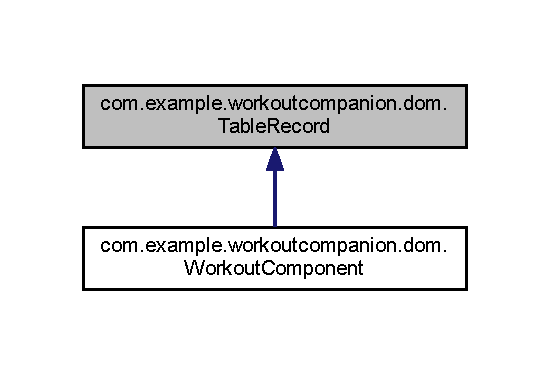
\includegraphics[width=264pt]{classcom_1_1example_1_1workoutcompanion_1_1dom_1_1_table_record__inherit__graph}
\end{center}
\end{figure}
\subsection*{Public Member Functions}
\begin{DoxyCompactItemize}
\item 
Long \hyperlink{classcom_1_1example_1_1workoutcompanion_1_1dom_1_1_table_record_aaad8f1c67d8e69fbc651322d5e40a2fc}{get\-I\-D} ()
\item 
void \hyperlink{classcom_1_1example_1_1workoutcompanion_1_1dom_1_1_table_record_a391da9c1bd03df54429f6b64602df2ce}{set\-I\-D} (Long a\-\_\-n\-I\-D)
\end{DoxyCompactItemize}
\subsection*{Protected Member Functions}
\begin{DoxyCompactItemize}
\item 
\hyperlink{classcom_1_1example_1_1workoutcompanion_1_1dom_1_1_table_record_af45541b51d998b04d359ffae63569773}{Table\-Record} ()
\end{DoxyCompactItemize}
\subsection*{Protected Attributes}
\begin{DoxyCompactItemize}
\item 
Long \hyperlink{classcom_1_1example_1_1workoutcompanion_1_1dom_1_1_table_record_a6810acfa101344b4ec1d901a69158086}{m\-\_\-n\-I\-D}
\end{DoxyCompactItemize}


\subsection{Constructor \& Destructor Documentation}
\hypertarget{classcom_1_1example_1_1workoutcompanion_1_1dom_1_1_table_record_af45541b51d998b04d359ffae63569773}{\index{com\-::example\-::workoutcompanion\-::dom\-::\-Table\-Record@{com\-::example\-::workoutcompanion\-::dom\-::\-Table\-Record}!Table\-Record@{Table\-Record}}
\index{Table\-Record@{Table\-Record}!com::example::workoutcompanion::dom::TableRecord@{com\-::example\-::workoutcompanion\-::dom\-::\-Table\-Record}}
\subsubsection[{Table\-Record}]{\setlength{\rightskip}{0pt plus 5cm}com.\-example.\-workoutcompanion.\-dom.\-Table\-Record.\-Table\-Record (
\begin{DoxyParamCaption}
{}
\end{DoxyParamCaption}
)\hspace{0.3cm}{\ttfamily [protected]}}}\label{classcom_1_1example_1_1workoutcompanion_1_1dom_1_1_table_record_af45541b51d998b04d359ffae63569773}


\subsection{Member Function Documentation}
\hypertarget{classcom_1_1example_1_1workoutcompanion_1_1dom_1_1_table_record_aaad8f1c67d8e69fbc651322d5e40a2fc}{\index{com\-::example\-::workoutcompanion\-::dom\-::\-Table\-Record@{com\-::example\-::workoutcompanion\-::dom\-::\-Table\-Record}!get\-I\-D@{get\-I\-D}}
\index{get\-I\-D@{get\-I\-D}!com::example::workoutcompanion::dom::TableRecord@{com\-::example\-::workoutcompanion\-::dom\-::\-Table\-Record}}
\subsubsection[{get\-I\-D}]{\setlength{\rightskip}{0pt plus 5cm}Long com.\-example.\-workoutcompanion.\-dom.\-Table\-Record.\-get\-I\-D (
\begin{DoxyParamCaption}
{}
\end{DoxyParamCaption}
)}}\label{classcom_1_1example_1_1workoutcompanion_1_1dom_1_1_table_record_aaad8f1c67d8e69fbc651322d5e40a2fc}
\hypertarget{classcom_1_1example_1_1workoutcompanion_1_1dom_1_1_table_record_a391da9c1bd03df54429f6b64602df2ce}{\index{com\-::example\-::workoutcompanion\-::dom\-::\-Table\-Record@{com\-::example\-::workoutcompanion\-::dom\-::\-Table\-Record}!set\-I\-D@{set\-I\-D}}
\index{set\-I\-D@{set\-I\-D}!com::example::workoutcompanion::dom::TableRecord@{com\-::example\-::workoutcompanion\-::dom\-::\-Table\-Record}}
\subsubsection[{set\-I\-D}]{\setlength{\rightskip}{0pt plus 5cm}void com.\-example.\-workoutcompanion.\-dom.\-Table\-Record.\-set\-I\-D (
\begin{DoxyParamCaption}
\item[{Long}]{a\-\_\-n\-I\-D}
\end{DoxyParamCaption}
)}}\label{classcom_1_1example_1_1workoutcompanion_1_1dom_1_1_table_record_a391da9c1bd03df54429f6b64602df2ce}


\subsection{Member Data Documentation}
\hypertarget{classcom_1_1example_1_1workoutcompanion_1_1dom_1_1_table_record_a6810acfa101344b4ec1d901a69158086}{\index{com\-::example\-::workoutcompanion\-::dom\-::\-Table\-Record@{com\-::example\-::workoutcompanion\-::dom\-::\-Table\-Record}!m\-\_\-n\-I\-D@{m\-\_\-n\-I\-D}}
\index{m\-\_\-n\-I\-D@{m\-\_\-n\-I\-D}!com::example::workoutcompanion::dom::TableRecord@{com\-::example\-::workoutcompanion\-::dom\-::\-Table\-Record}}
\subsubsection[{m\-\_\-n\-I\-D}]{\setlength{\rightskip}{0pt plus 5cm}Long com.\-example.\-workoutcompanion.\-dom.\-Table\-Record.\-m\-\_\-n\-I\-D\hspace{0.3cm}{\ttfamily [protected]}}}\label{classcom_1_1example_1_1workoutcompanion_1_1dom_1_1_table_record_a6810acfa101344b4ec1d901a69158086}


The documentation for this class was generated from the following file\-:\begin{DoxyCompactItemize}
\item 
Desktop/git\-\_\-proj/workout/src/com/example/workoutcompanion/dom/\hyperlink{_table_record_8java}{Table\-Record.\-java}\end{DoxyCompactItemize}

\hypertarget{classcom_1_1example_1_1workoutcompanion_1_1dom_1_1_workout}{\section{com.\-example.\-workoutcompanion.\-dom.\-Workout Class Reference}
\label{classcom_1_1example_1_1workoutcompanion_1_1dom_1_1_workout}\index{com.\-example.\-workoutcompanion.\-dom.\-Workout@{com.\-example.\-workoutcompanion.\-dom.\-Workout}}
}
\subsection*{Public Member Functions}
\begin{DoxyCompactItemize}
\item 
\hyperlink{classcom_1_1example_1_1workoutcompanion_1_1dom_1_1_workout_a659d9313e861a95d04075615f383e564}{Workout} (String a\-\_\-s\-Name)
\item 
String \hyperlink{classcom_1_1example_1_1workoutcompanion_1_1dom_1_1_workout_adda3e121b7c0ecf1fa80c272dc5218aa}{get\-Name} ()
\item 
void \hyperlink{classcom_1_1example_1_1workoutcompanion_1_1dom_1_1_workout_a11e053688dec0a5a527c885610338b1b}{set\-Name} (String name)
\item 
Foreign\-Collection$<$ \hyperlink{classcom_1_1example_1_1workoutcompanion_1_1dom_1_1_exercise}{Exercise} $>$ \hyperlink{classcom_1_1example_1_1workoutcompanion_1_1dom_1_1_workout_ac9c0c14bad6cbd7a6d18c753bddd6c50}{get\-Exercises} ()
\end{DoxyCompactItemize}
\subsection*{Static Public Attributes}
\begin{DoxyCompactItemize}
\item 
static final String \hyperlink{classcom_1_1example_1_1workoutcompanion_1_1dom_1_1_workout_a18f5c457f9aa5822f652f8a920f2ac9a}{W\-O\-R\-K\-O\-U\-T\-\_\-\-N\-A\-M\-E\-\_\-\-C\-O\-L\-U\-M\-N\-\_\-\-F\-I\-E\-L\-D} = \char`\"{}name\char`\"{}
\end{DoxyCompactItemize}


\subsection{Constructor \& Destructor Documentation}
\hypertarget{classcom_1_1example_1_1workoutcompanion_1_1dom_1_1_workout_a659d9313e861a95d04075615f383e564}{\index{com\-::example\-::workoutcompanion\-::dom\-::\-Workout@{com\-::example\-::workoutcompanion\-::dom\-::\-Workout}!Workout@{Workout}}
\index{Workout@{Workout}!com::example::workoutcompanion::dom::Workout@{com\-::example\-::workoutcompanion\-::dom\-::\-Workout}}
\subsubsection[{Workout}]{\setlength{\rightskip}{0pt plus 5cm}com.\-example.\-workoutcompanion.\-dom.\-Workout.\-Workout (
\begin{DoxyParamCaption}
\item[{String}]{a\-\_\-s\-Name}
\end{DoxyParamCaption}
)}}\label{classcom_1_1example_1_1workoutcompanion_1_1dom_1_1_workout_a659d9313e861a95d04075615f383e564}


\subsection{Member Function Documentation}
\hypertarget{classcom_1_1example_1_1workoutcompanion_1_1dom_1_1_workout_ac9c0c14bad6cbd7a6d18c753bddd6c50}{\index{com\-::example\-::workoutcompanion\-::dom\-::\-Workout@{com\-::example\-::workoutcompanion\-::dom\-::\-Workout}!get\-Exercises@{get\-Exercises}}
\index{get\-Exercises@{get\-Exercises}!com::example::workoutcompanion::dom::Workout@{com\-::example\-::workoutcompanion\-::dom\-::\-Workout}}
\subsubsection[{get\-Exercises}]{\setlength{\rightskip}{0pt plus 5cm}Foreign\-Collection$<${\bf Exercise}$>$ com.\-example.\-workoutcompanion.\-dom.\-Workout.\-get\-Exercises (
\begin{DoxyParamCaption}
{}
\end{DoxyParamCaption}
)}}\label{classcom_1_1example_1_1workoutcompanion_1_1dom_1_1_workout_ac9c0c14bad6cbd7a6d18c753bddd6c50}
\hypertarget{classcom_1_1example_1_1workoutcompanion_1_1dom_1_1_workout_adda3e121b7c0ecf1fa80c272dc5218aa}{\index{com\-::example\-::workoutcompanion\-::dom\-::\-Workout@{com\-::example\-::workoutcompanion\-::dom\-::\-Workout}!get\-Name@{get\-Name}}
\index{get\-Name@{get\-Name}!com::example::workoutcompanion::dom::Workout@{com\-::example\-::workoutcompanion\-::dom\-::\-Workout}}
\subsubsection[{get\-Name}]{\setlength{\rightskip}{0pt plus 5cm}String com.\-example.\-workoutcompanion.\-dom.\-Workout.\-get\-Name (
\begin{DoxyParamCaption}
{}
\end{DoxyParamCaption}
)}}\label{classcom_1_1example_1_1workoutcompanion_1_1dom_1_1_workout_adda3e121b7c0ecf1fa80c272dc5218aa}
\hypertarget{classcom_1_1example_1_1workoutcompanion_1_1dom_1_1_workout_a11e053688dec0a5a527c885610338b1b}{\index{com\-::example\-::workoutcompanion\-::dom\-::\-Workout@{com\-::example\-::workoutcompanion\-::dom\-::\-Workout}!set\-Name@{set\-Name}}
\index{set\-Name@{set\-Name}!com::example::workoutcompanion::dom::Workout@{com\-::example\-::workoutcompanion\-::dom\-::\-Workout}}
\subsubsection[{set\-Name}]{\setlength{\rightskip}{0pt plus 5cm}void com.\-example.\-workoutcompanion.\-dom.\-Workout.\-set\-Name (
\begin{DoxyParamCaption}
\item[{String}]{name}
\end{DoxyParamCaption}
)}}\label{classcom_1_1example_1_1workoutcompanion_1_1dom_1_1_workout_a11e053688dec0a5a527c885610338b1b}


\subsection{Member Data Documentation}
\hypertarget{classcom_1_1example_1_1workoutcompanion_1_1dom_1_1_workout_a18f5c457f9aa5822f652f8a920f2ac9a}{\index{com\-::example\-::workoutcompanion\-::dom\-::\-Workout@{com\-::example\-::workoutcompanion\-::dom\-::\-Workout}!W\-O\-R\-K\-O\-U\-T\-\_\-\-N\-A\-M\-E\-\_\-\-C\-O\-L\-U\-M\-N\-\_\-\-F\-I\-E\-L\-D@{W\-O\-R\-K\-O\-U\-T\-\_\-\-N\-A\-M\-E\-\_\-\-C\-O\-L\-U\-M\-N\-\_\-\-F\-I\-E\-L\-D}}
\index{W\-O\-R\-K\-O\-U\-T\-\_\-\-N\-A\-M\-E\-\_\-\-C\-O\-L\-U\-M\-N\-\_\-\-F\-I\-E\-L\-D@{W\-O\-R\-K\-O\-U\-T\-\_\-\-N\-A\-M\-E\-\_\-\-C\-O\-L\-U\-M\-N\-\_\-\-F\-I\-E\-L\-D}!com::example::workoutcompanion::dom::Workout@{com\-::example\-::workoutcompanion\-::dom\-::\-Workout}}
\subsubsection[{W\-O\-R\-K\-O\-U\-T\-\_\-\-N\-A\-M\-E\-\_\-\-C\-O\-L\-U\-M\-N\-\_\-\-F\-I\-E\-L\-D}]{\setlength{\rightskip}{0pt plus 5cm}final String com.\-example.\-workoutcompanion.\-dom.\-Workout.\-W\-O\-R\-K\-O\-U\-T\-\_\-\-N\-A\-M\-E\-\_\-\-C\-O\-L\-U\-M\-N\-\_\-\-F\-I\-E\-L\-D = \char`\"{}name\char`\"{}\hspace{0.3cm}{\ttfamily [static]}}}\label{classcom_1_1example_1_1workoutcompanion_1_1dom_1_1_workout_a18f5c457f9aa5822f652f8a920f2ac9a}


The documentation for this class was generated from the following file\-:\begin{DoxyCompactItemize}
\item 
Desktop/git\-\_\-proj/workout/src/com/example/workoutcompanion/dom/\hyperlink{_workout_8java}{Workout.\-java}\end{DoxyCompactItemize}

\hypertarget{classcom_1_1example_1_1workoutcompanion_1_1_workout_activity}{\section{com.\-example.\-workoutcompanion.\-Workout\-Activity Class Reference}
\label{classcom_1_1example_1_1workoutcompanion_1_1_workout_activity}\index{com.\-example.\-workoutcompanion.\-Workout\-Activity@{com.\-example.\-workoutcompanion.\-Workout\-Activity}}
}


Inheritance diagram for com.\-example.\-workoutcompanion.\-Workout\-Activity\-:\nopagebreak
\begin{figure}[H]
\begin{center}
\leavevmode
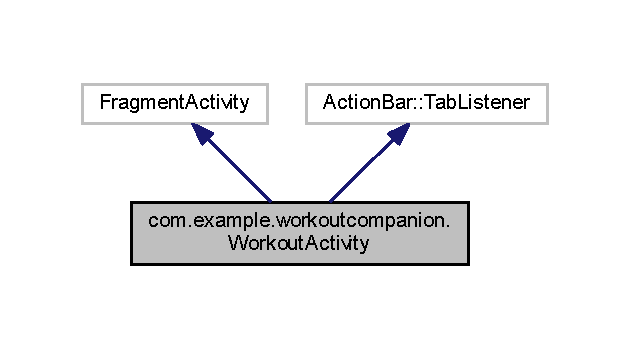
\includegraphics[width=303pt]{classcom_1_1example_1_1workoutcompanion_1_1_workout_activity__inherit__graph}
\end{center}
\end{figure}


Collaboration diagram for com.\-example.\-workoutcompanion.\-Workout\-Activity\-:
\nopagebreak
\begin{figure}[H]
\begin{center}
\leavevmode
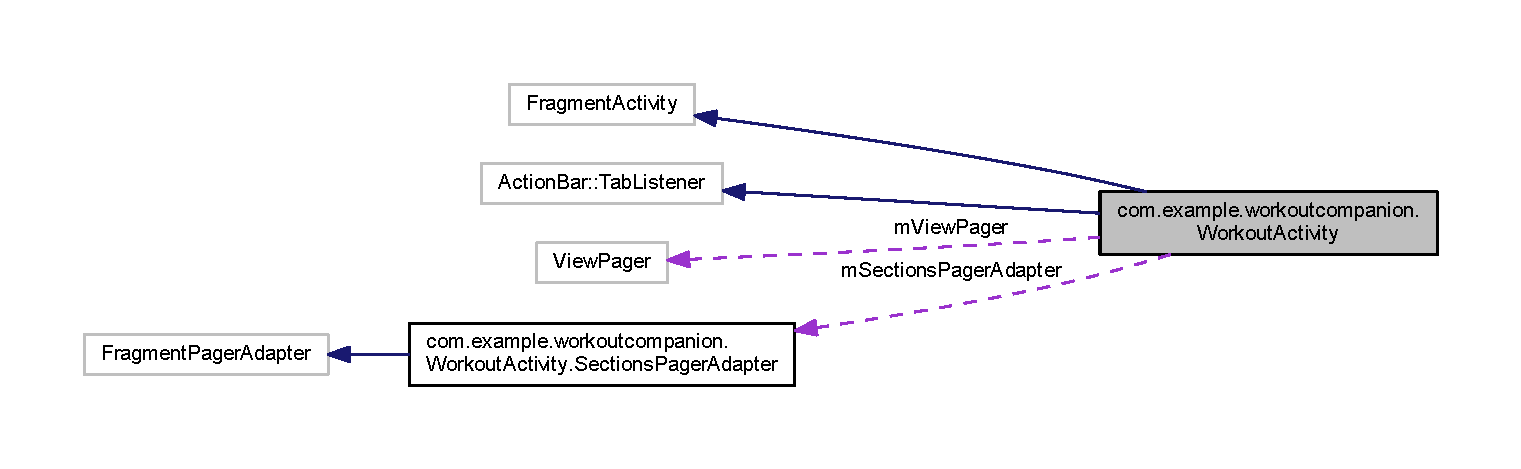
\includegraphics[width=350pt]{classcom_1_1example_1_1workoutcompanion_1_1_workout_activity__coll__graph}
\end{center}
\end{figure}
\subsection*{Classes}
\begin{DoxyCompactItemize}
\item 
class {\bfseries Dummy\-Section\-Fragment}
\end{DoxyCompactItemize}
\subsection*{Public Member Functions}
\begin{DoxyCompactItemize}
\item 
boolean \hyperlink{classcom_1_1example_1_1workoutcompanion_1_1_workout_activity_ae06438356b251373878b8355e48dbeeb}{on\-Create\-Options\-Menu} (Menu menu)
\item 
void \hyperlink{classcom_1_1example_1_1workoutcompanion_1_1_workout_activity_a058429dd9b85af3a68938d753caaaed0}{on\-Tab\-Selected} (Action\-Bar.\-Tab tab, Fragment\-Transaction fragment\-Transaction)
\item 
void \hyperlink{classcom_1_1example_1_1workoutcompanion_1_1_workout_activity_a59bf7cbca8c0dc7d29df3633facce3e7}{on\-Tab\-Unselected} (Action\-Bar.\-Tab tab, Fragment\-Transaction fragment\-Transaction)
\item 
void \hyperlink{classcom_1_1example_1_1workoutcompanion_1_1_workout_activity_a030d02894f9f27ddbfc318e8ffbbedef}{on\-Tab\-Reselected} (Action\-Bar.\-Tab tab, Fragment\-Transaction fragment\-Transaction)
\end{DoxyCompactItemize}
\subsection*{Public Attributes}
\begin{DoxyCompactItemize}
\item 
\hyperlink{classcom_1_1example_1_1workoutcompanion_1_1dom_1_1_profile}{Profile} \hyperlink{classcom_1_1example_1_1workoutcompanion_1_1_workout_activity_a869892c117ac8470219446dfba839688}{profile}
\end{DoxyCompactItemize}
\subsection*{Protected Member Functions}
\begin{DoxyCompactItemize}
\item 
void \hyperlink{classcom_1_1example_1_1workoutcompanion_1_1_workout_activity_ae63e0efa8659a02d91e8db8332a77c24}{on\-Create} (Bundle saved\-Instance\-State)
\end{DoxyCompactItemize}


\subsection{Member Function Documentation}
\hypertarget{classcom_1_1example_1_1workoutcompanion_1_1_workout_activity_ae63e0efa8659a02d91e8db8332a77c24}{\index{com\-::example\-::workoutcompanion\-::\-Workout\-Activity@{com\-::example\-::workoutcompanion\-::\-Workout\-Activity}!on\-Create@{on\-Create}}
\index{on\-Create@{on\-Create}!com::example::workoutcompanion::WorkoutActivity@{com\-::example\-::workoutcompanion\-::\-Workout\-Activity}}
\subsubsection[{on\-Create}]{\setlength{\rightskip}{0pt plus 5cm}void com.\-example.\-workoutcompanion.\-Workout\-Activity.\-on\-Create (
\begin{DoxyParamCaption}
\item[{Bundle}]{saved\-Instance\-State}
\end{DoxyParamCaption}
)\hspace{0.3cm}{\ttfamily [protected]}}}\label{classcom_1_1example_1_1workoutcompanion_1_1_workout_activity_ae63e0efa8659a02d91e8db8332a77c24}
\hypertarget{classcom_1_1example_1_1workoutcompanion_1_1_workout_activity_ae06438356b251373878b8355e48dbeeb}{\index{com\-::example\-::workoutcompanion\-::\-Workout\-Activity@{com\-::example\-::workoutcompanion\-::\-Workout\-Activity}!on\-Create\-Options\-Menu@{on\-Create\-Options\-Menu}}
\index{on\-Create\-Options\-Menu@{on\-Create\-Options\-Menu}!com::example::workoutcompanion::WorkoutActivity@{com\-::example\-::workoutcompanion\-::\-Workout\-Activity}}
\subsubsection[{on\-Create\-Options\-Menu}]{\setlength{\rightskip}{0pt plus 5cm}boolean com.\-example.\-workoutcompanion.\-Workout\-Activity.\-on\-Create\-Options\-Menu (
\begin{DoxyParamCaption}
\item[{Menu}]{menu}
\end{DoxyParamCaption}
)}}\label{classcom_1_1example_1_1workoutcompanion_1_1_workout_activity_ae06438356b251373878b8355e48dbeeb}
\hypertarget{classcom_1_1example_1_1workoutcompanion_1_1_workout_activity_a030d02894f9f27ddbfc318e8ffbbedef}{\index{com\-::example\-::workoutcompanion\-::\-Workout\-Activity@{com\-::example\-::workoutcompanion\-::\-Workout\-Activity}!on\-Tab\-Reselected@{on\-Tab\-Reselected}}
\index{on\-Tab\-Reselected@{on\-Tab\-Reselected}!com::example::workoutcompanion::WorkoutActivity@{com\-::example\-::workoutcompanion\-::\-Workout\-Activity}}
\subsubsection[{on\-Tab\-Reselected}]{\setlength{\rightskip}{0pt plus 5cm}void com.\-example.\-workoutcompanion.\-Workout\-Activity.\-on\-Tab\-Reselected (
\begin{DoxyParamCaption}
\item[{Action\-Bar.\-Tab}]{tab, }
\item[{Fragment\-Transaction}]{fragment\-Transaction}
\end{DoxyParamCaption}
)}}\label{classcom_1_1example_1_1workoutcompanion_1_1_workout_activity_a030d02894f9f27ddbfc318e8ffbbedef}
\hypertarget{classcom_1_1example_1_1workoutcompanion_1_1_workout_activity_a058429dd9b85af3a68938d753caaaed0}{\index{com\-::example\-::workoutcompanion\-::\-Workout\-Activity@{com\-::example\-::workoutcompanion\-::\-Workout\-Activity}!on\-Tab\-Selected@{on\-Tab\-Selected}}
\index{on\-Tab\-Selected@{on\-Tab\-Selected}!com::example::workoutcompanion::WorkoutActivity@{com\-::example\-::workoutcompanion\-::\-Workout\-Activity}}
\subsubsection[{on\-Tab\-Selected}]{\setlength{\rightskip}{0pt plus 5cm}void com.\-example.\-workoutcompanion.\-Workout\-Activity.\-on\-Tab\-Selected (
\begin{DoxyParamCaption}
\item[{Action\-Bar.\-Tab}]{tab, }
\item[{Fragment\-Transaction}]{fragment\-Transaction}
\end{DoxyParamCaption}
)}}\label{classcom_1_1example_1_1workoutcompanion_1_1_workout_activity_a058429dd9b85af3a68938d753caaaed0}
\hypertarget{classcom_1_1example_1_1workoutcompanion_1_1_workout_activity_a59bf7cbca8c0dc7d29df3633facce3e7}{\index{com\-::example\-::workoutcompanion\-::\-Workout\-Activity@{com\-::example\-::workoutcompanion\-::\-Workout\-Activity}!on\-Tab\-Unselected@{on\-Tab\-Unselected}}
\index{on\-Tab\-Unselected@{on\-Tab\-Unselected}!com::example::workoutcompanion::WorkoutActivity@{com\-::example\-::workoutcompanion\-::\-Workout\-Activity}}
\subsubsection[{on\-Tab\-Unselected}]{\setlength{\rightskip}{0pt plus 5cm}void com.\-example.\-workoutcompanion.\-Workout\-Activity.\-on\-Tab\-Unselected (
\begin{DoxyParamCaption}
\item[{Action\-Bar.\-Tab}]{tab, }
\item[{Fragment\-Transaction}]{fragment\-Transaction}
\end{DoxyParamCaption}
)}}\label{classcom_1_1example_1_1workoutcompanion_1_1_workout_activity_a59bf7cbca8c0dc7d29df3633facce3e7}


\subsection{Member Data Documentation}
\hypertarget{classcom_1_1example_1_1workoutcompanion_1_1_workout_activity_a869892c117ac8470219446dfba839688}{\index{com\-::example\-::workoutcompanion\-::\-Workout\-Activity@{com\-::example\-::workoutcompanion\-::\-Workout\-Activity}!profile@{profile}}
\index{profile@{profile}!com::example::workoutcompanion::WorkoutActivity@{com\-::example\-::workoutcompanion\-::\-Workout\-Activity}}
\subsubsection[{profile}]{\setlength{\rightskip}{0pt plus 5cm}{\bf Profile} com.\-example.\-workoutcompanion.\-Workout\-Activity.\-profile}}\label{classcom_1_1example_1_1workoutcompanion_1_1_workout_activity_a869892c117ac8470219446dfba839688}


The documentation for this class was generated from the following file\-:\begin{DoxyCompactItemize}
\item 
Desktop/git\-\_\-proj/workout/src/com/example/workoutcompanion/\hyperlink{_workout_activity_8java}{Workout\-Activity.\-java}\end{DoxyCompactItemize}

\hypertarget{classcom_1_1example_1_1workoutcompanion_1_1dom_1_1_workout_component}{\section{com.\-example.\-workoutcompanion.\-dom.\-Workout\-Component Class Reference}
\label{classcom_1_1example_1_1workoutcompanion_1_1dom_1_1_workout_component}\index{com.\-example.\-workoutcompanion.\-dom.\-Workout\-Component@{com.\-example.\-workoutcompanion.\-dom.\-Workout\-Component}}
}


Inheritance diagram for com.\-example.\-workoutcompanion.\-dom.\-Workout\-Component\-:
\nopagebreak
\begin{figure}[H]
\begin{center}
\leavevmode
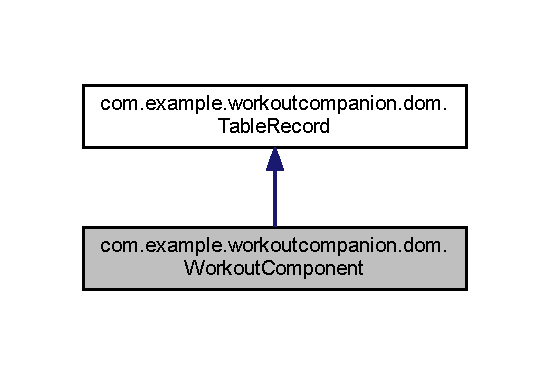
\includegraphics[width=264pt]{classcom_1_1example_1_1workoutcompanion_1_1dom_1_1_workout_component__inherit__graph}
\end{center}
\end{figure}


Collaboration diagram for com.\-example.\-workoutcompanion.\-dom.\-Workout\-Component\-:
\nopagebreak
\begin{figure}[H]
\begin{center}
\leavevmode
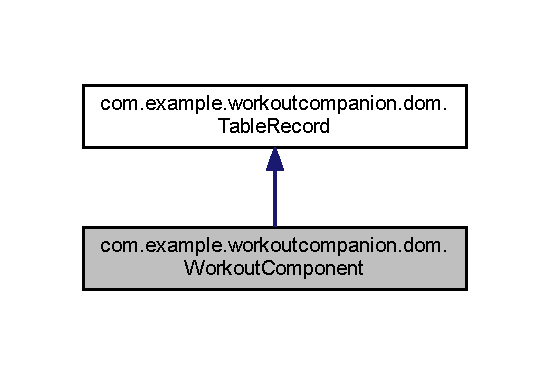
\includegraphics[width=264pt]{classcom_1_1example_1_1workoutcompanion_1_1dom_1_1_workout_component__coll__graph}
\end{center}
\end{figure}
\subsection*{Public Member Functions}
\begin{DoxyCompactItemize}
\item 
String \hyperlink{classcom_1_1example_1_1workoutcompanion_1_1dom_1_1_workout_component_ac5ed7ef5dca690ce545aaeb06b814161}{get\-Name} ()
\item 
void \hyperlink{classcom_1_1example_1_1workoutcompanion_1_1dom_1_1_workout_component_a9516bf277c5120c27ab36d4488946720}{set\-Name} (String \hyperlink{classcom_1_1example_1_1workoutcompanion_1_1dom_1_1_workout_component_aea36d36e652e5d7501135663a7a1148f}{m\-\_\-s\-Name})
\end{DoxyCompactItemize}
\subsection*{Protected Member Functions}
\begin{DoxyCompactItemize}
\item 
\hyperlink{classcom_1_1example_1_1workoutcompanion_1_1dom_1_1_workout_component_a95622d028ee393712cf4782ab0ae5956}{Workout\-Component} (String a\-\_\-s\-Name)
\end{DoxyCompactItemize}
\subsection*{Protected Attributes}
\begin{DoxyCompactItemize}
\item 
String \hyperlink{classcom_1_1example_1_1workoutcompanion_1_1dom_1_1_workout_component_aea36d36e652e5d7501135663a7a1148f}{m\-\_\-s\-Name}
\end{DoxyCompactItemize}


\subsection{Constructor \& Destructor Documentation}
\hypertarget{classcom_1_1example_1_1workoutcompanion_1_1dom_1_1_workout_component_a95622d028ee393712cf4782ab0ae5956}{\index{com\-::example\-::workoutcompanion\-::dom\-::\-Workout\-Component@{com\-::example\-::workoutcompanion\-::dom\-::\-Workout\-Component}!Workout\-Component@{Workout\-Component}}
\index{Workout\-Component@{Workout\-Component}!com::example::workoutcompanion::dom::WorkoutComponent@{com\-::example\-::workoutcompanion\-::dom\-::\-Workout\-Component}}
\subsubsection[{Workout\-Component}]{\setlength{\rightskip}{0pt plus 5cm}com.\-example.\-workoutcompanion.\-dom.\-Workout\-Component.\-Workout\-Component (
\begin{DoxyParamCaption}
\item[{String}]{a\-\_\-s\-Name}
\end{DoxyParamCaption}
)\hspace{0.3cm}{\ttfamily [protected]}}}\label{classcom_1_1example_1_1workoutcompanion_1_1dom_1_1_workout_component_a95622d028ee393712cf4782ab0ae5956}


\subsection{Member Function Documentation}
\hypertarget{classcom_1_1example_1_1workoutcompanion_1_1dom_1_1_workout_component_ac5ed7ef5dca690ce545aaeb06b814161}{\index{com\-::example\-::workoutcompanion\-::dom\-::\-Workout\-Component@{com\-::example\-::workoutcompanion\-::dom\-::\-Workout\-Component}!get\-Name@{get\-Name}}
\index{get\-Name@{get\-Name}!com::example::workoutcompanion::dom::WorkoutComponent@{com\-::example\-::workoutcompanion\-::dom\-::\-Workout\-Component}}
\subsubsection[{get\-Name}]{\setlength{\rightskip}{0pt plus 5cm}String com.\-example.\-workoutcompanion.\-dom.\-Workout\-Component.\-get\-Name (
\begin{DoxyParamCaption}
{}
\end{DoxyParamCaption}
)}}\label{classcom_1_1example_1_1workoutcompanion_1_1dom_1_1_workout_component_ac5ed7ef5dca690ce545aaeb06b814161}
\hypertarget{classcom_1_1example_1_1workoutcompanion_1_1dom_1_1_workout_component_a9516bf277c5120c27ab36d4488946720}{\index{com\-::example\-::workoutcompanion\-::dom\-::\-Workout\-Component@{com\-::example\-::workoutcompanion\-::dom\-::\-Workout\-Component}!set\-Name@{set\-Name}}
\index{set\-Name@{set\-Name}!com::example::workoutcompanion::dom::WorkoutComponent@{com\-::example\-::workoutcompanion\-::dom\-::\-Workout\-Component}}
\subsubsection[{set\-Name}]{\setlength{\rightskip}{0pt plus 5cm}void com.\-example.\-workoutcompanion.\-dom.\-Workout\-Component.\-set\-Name (
\begin{DoxyParamCaption}
\item[{String}]{m\-\_\-s\-Name}
\end{DoxyParamCaption}
)}}\label{classcom_1_1example_1_1workoutcompanion_1_1dom_1_1_workout_component_a9516bf277c5120c27ab36d4488946720}


\subsection{Member Data Documentation}
\hypertarget{classcom_1_1example_1_1workoutcompanion_1_1dom_1_1_workout_component_aea36d36e652e5d7501135663a7a1148f}{\index{com\-::example\-::workoutcompanion\-::dom\-::\-Workout\-Component@{com\-::example\-::workoutcompanion\-::dom\-::\-Workout\-Component}!m\-\_\-s\-Name@{m\-\_\-s\-Name}}
\index{m\-\_\-s\-Name@{m\-\_\-s\-Name}!com::example::workoutcompanion::dom::WorkoutComponent@{com\-::example\-::workoutcompanion\-::dom\-::\-Workout\-Component}}
\subsubsection[{m\-\_\-s\-Name}]{\setlength{\rightskip}{0pt plus 5cm}String com.\-example.\-workoutcompanion.\-dom.\-Workout\-Component.\-m\-\_\-s\-Name\hspace{0.3cm}{\ttfamily [protected]}}}\label{classcom_1_1example_1_1workoutcompanion_1_1dom_1_1_workout_component_aea36d36e652e5d7501135663a7a1148f}


The documentation for this class was generated from the following file\-:\begin{DoxyCompactItemize}
\item 
Desktop/git\-\_\-proj/workout/src/com/example/workoutcompanion/dom/\hyperlink{_workout_component_8java}{Workout\-Component.\-java}\end{DoxyCompactItemize}

\chapter{File Documentation}
\hypertarget{_build_config_8java}{\section{Desktop/git\-\_\-proj/workout/gen/com/example/workoutcompanion/\-Build\-Config.java File Reference}
\label{_build_config_8java}\index{Desktop/git\-\_\-proj/workout/gen/com/example/workoutcompanion/\-Build\-Config.\-java@{Desktop/git\-\_\-proj/workout/gen/com/example/workoutcompanion/\-Build\-Config.\-java}}
}
\subsection*{Classes}
\begin{DoxyCompactItemize}
\item 
class \hyperlink{classcom_1_1example_1_1workoutcompanion_1_1_build_config}{com.\-example.\-workoutcompanion.\-Build\-Config}
\end{DoxyCompactItemize}
\subsection*{Packages}
\begin{DoxyCompactItemize}
\item 
package \hyperlink{namespacecom_1_1example_1_1workoutcompanion}{com.\-example.\-workoutcompanion}
\end{DoxyCompactItemize}

\hypertarget{_r_8java}{\section{Desktop/git\-\_\-proj/workout/gen/com/example/workoutcompanion/\-R.java File Reference}
\label{_r_8java}\index{Desktop/git\-\_\-proj/workout/gen/com/example/workoutcompanion/\-R.\-java@{Desktop/git\-\_\-proj/workout/gen/com/example/workoutcompanion/\-R.\-java}}
}
\subsection*{Classes}
\begin{DoxyCompactItemize}
\item 
class \hyperlink{classcom_1_1example_1_1workoutcompanion_1_1_r}{com.\-example.\-workoutcompanion.\-R}
\item 
class {\bfseries com.\-example.\-workoutcompanion.\-R.\-attr}
\item 
class {\bfseries com.\-example.\-workoutcompanion.\-R.\-dimen}
\item 
class {\bfseries com.\-example.\-workoutcompanion.\-R.\-drawable}
\item 
class {\bfseries com.\-example.\-workoutcompanion.\-R.\-id}
\item 
class {\bfseries com.\-example.\-workoutcompanion.\-R.\-layout}
\item 
class {\bfseries com.\-example.\-workoutcompanion.\-R.\-menu}
\item 
class {\bfseries com.\-example.\-workoutcompanion.\-R.\-string}
\item 
class {\bfseries com.\-example.\-workoutcompanion.\-R.\-style}
\end{DoxyCompactItemize}
\subsection*{Packages}
\begin{DoxyCompactItemize}
\item 
package \hyperlink{namespacecom_1_1example_1_1workoutcompanion}{com.\-example.\-workoutcompanion}
\end{DoxyCompactItemize}

\hypertarget{_add_exercise_to_workout_cmd_8java}{\section{Desktop/git\-\_\-proj/workout/src/com/example/workoutcompanion/controller/\-Add\-Exercise\-To\-Workout\-Cmd.java File Reference}
\label{_add_exercise_to_workout_cmd_8java}\index{Desktop/git\-\_\-proj/workout/src/com/example/workoutcompanion/controller/\-Add\-Exercise\-To\-Workout\-Cmd.\-java@{Desktop/git\-\_\-proj/workout/src/com/example/workoutcompanion/controller/\-Add\-Exercise\-To\-Workout\-Cmd.\-java}}
}
\subsection*{Classes}
\begin{DoxyCompactItemize}
\item 
class \hyperlink{classcom_1_1example_1_1workoutcompanion_1_1controller_1_1_add_exercise_to_workout_cmd}{com.\-example.\-workoutcompanion.\-controller.\-Add\-Exercise\-To\-Workout\-Cmd}
\end{DoxyCompactItemize}
\subsection*{Packages}
\begin{DoxyCompactItemize}
\item 
package \hyperlink{namespacecom_1_1example_1_1workoutcompanion_1_1controller}{com.\-example.\-workoutcompanion.\-controller}
\end{DoxyCompactItemize}

\hypertarget{_command_8java}{\section{Desktop/git\-\_\-proj/workout/src/com/example/workoutcompanion/controller/\-Command.java File Reference}
\label{_command_8java}\index{Desktop/git\-\_\-proj/workout/src/com/example/workoutcompanion/controller/\-Command.\-java@{Desktop/git\-\_\-proj/workout/src/com/example/workoutcompanion/controller/\-Command.\-java}}
}
\subsection*{Classes}
\begin{DoxyCompactItemize}
\item 
interface \hyperlink{interfacecom_1_1example_1_1workoutcompanion_1_1controller_1_1_command}{com.\-example.\-workoutcompanion.\-controller.\-Command}
\end{DoxyCompactItemize}
\subsection*{Packages}
\begin{DoxyCompactItemize}
\item 
package \hyperlink{namespacecom_1_1example_1_1workoutcompanion_1_1controller}{com.\-example.\-workoutcompanion.\-controller}
\end{DoxyCompactItemize}

\hypertarget{_controller_8java}{\section{Desktop/git\-\_\-proj/workout/src/com/example/workoutcompanion/controller/\-Controller.java File Reference}
\label{_controller_8java}\index{Desktop/git\-\_\-proj/workout/src/com/example/workoutcompanion/controller/\-Controller.\-java@{Desktop/git\-\_\-proj/workout/src/com/example/workoutcompanion/controller/\-Controller.\-java}}
}
\subsection*{Classes}
\begin{DoxyCompactItemize}
\item 
class \hyperlink{classcom_1_1example_1_1workoutcompanion_1_1controller_1_1_controller}{com.\-example.\-workoutcompanion.\-controller.\-Controller}
\end{DoxyCompactItemize}
\subsection*{Packages}
\begin{DoxyCompactItemize}
\item 
package \hyperlink{namespacecom_1_1example_1_1workoutcompanion_1_1controller}{com.\-example.\-workoutcompanion.\-controller}
\end{DoxyCompactItemize}

\hypertarget{_create_exercise_cmd_8java}{\section{Desktop/git\-\_\-proj/workout/src/com/example/workoutcompanion/controller/\-Create\-Exercise\-Cmd.java File Reference}
\label{_create_exercise_cmd_8java}\index{Desktop/git\-\_\-proj/workout/src/com/example/workoutcompanion/controller/\-Create\-Exercise\-Cmd.\-java@{Desktop/git\-\_\-proj/workout/src/com/example/workoutcompanion/controller/\-Create\-Exercise\-Cmd.\-java}}
}
\subsection*{Classes}
\begin{DoxyCompactItemize}
\item 
class \hyperlink{classcom_1_1example_1_1workoutcompanion_1_1controller_1_1_create_exercise_cmd}{com.\-example.\-workoutcompanion.\-controller.\-Create\-Exercise\-Cmd}
\end{DoxyCompactItemize}
\subsection*{Packages}
\begin{DoxyCompactItemize}
\item 
package \hyperlink{namespacecom_1_1example_1_1workoutcompanion_1_1controller}{com.\-example.\-workoutcompanion.\-controller}
\end{DoxyCompactItemize}

\hypertarget{_create_workout_cmd_8java}{\section{Desktop/git\-\_\-proj/workout/src/com/example/workoutcompanion/controller/\-Create\-Workout\-Cmd.java File Reference}
\label{_create_workout_cmd_8java}\index{Desktop/git\-\_\-proj/workout/src/com/example/workoutcompanion/controller/\-Create\-Workout\-Cmd.\-java@{Desktop/git\-\_\-proj/workout/src/com/example/workoutcompanion/controller/\-Create\-Workout\-Cmd.\-java}}
}
\subsection*{Classes}
\begin{DoxyCompactItemize}
\item 
class \hyperlink{classcom_1_1example_1_1workoutcompanion_1_1controller_1_1_create_workout_cmd}{com.\-example.\-workoutcompanion.\-controller.\-Create\-Workout\-Cmd}
\end{DoxyCompactItemize}
\subsection*{Packages}
\begin{DoxyCompactItemize}
\item 
package \hyperlink{namespacecom_1_1example_1_1workoutcompanion_1_1controller}{com.\-example.\-workoutcompanion.\-controller}
\end{DoxyCompactItemize}

\hypertarget{_edit_exercise_cmd_8java}{\section{Desktop/git\-\_\-proj/workout/src/com/example/workoutcompanion/controller/\-Edit\-Exercise\-Cmd.java File Reference}
\label{_edit_exercise_cmd_8java}\index{Desktop/git\-\_\-proj/workout/src/com/example/workoutcompanion/controller/\-Edit\-Exercise\-Cmd.\-java@{Desktop/git\-\_\-proj/workout/src/com/example/workoutcompanion/controller/\-Edit\-Exercise\-Cmd.\-java}}
}
\subsection*{Classes}
\begin{DoxyCompactItemize}
\item 
class \hyperlink{classcom_1_1example_1_1workoutcompanion_1_1controller_1_1_edit_exercise_cmd}{com.\-example.\-workoutcompanion.\-controller.\-Edit\-Exercise\-Cmd}
\end{DoxyCompactItemize}
\subsection*{Packages}
\begin{DoxyCompactItemize}
\item 
package \hyperlink{namespacecom_1_1example_1_1workoutcompanion_1_1controller}{com.\-example.\-workoutcompanion.\-controller}
\end{DoxyCompactItemize}

\hypertarget{_edit_profile_cmd_8java}{\section{Desktop/git\-\_\-proj/workout/src/com/example/workoutcompanion/controller/\-Edit\-Profile\-Cmd.java File Reference}
\label{_edit_profile_cmd_8java}\index{Desktop/git\-\_\-proj/workout/src/com/example/workoutcompanion/controller/\-Edit\-Profile\-Cmd.\-java@{Desktop/git\-\_\-proj/workout/src/com/example/workoutcompanion/controller/\-Edit\-Profile\-Cmd.\-java}}
}
\subsection*{Classes}
\begin{DoxyCompactItemize}
\item 
class \hyperlink{classcom_1_1example_1_1workoutcompanion_1_1controller_1_1_edit_profile_cmd}{com.\-example.\-workoutcompanion.\-controller.\-Edit\-Profile\-Cmd}
\end{DoxyCompactItemize}
\subsection*{Packages}
\begin{DoxyCompactItemize}
\item 
package \hyperlink{namespacecom_1_1example_1_1workoutcompanion_1_1controller}{com.\-example.\-workoutcompanion.\-controller}
\end{DoxyCompactItemize}

\hypertarget{_edit_workout_cmd_8java}{\section{Desktop/git\-\_\-proj/workout/src/com/example/workoutcompanion/controller/\-Edit\-Workout\-Cmd.java File Reference}
\label{_edit_workout_cmd_8java}\index{Desktop/git\-\_\-proj/workout/src/com/example/workoutcompanion/controller/\-Edit\-Workout\-Cmd.\-java@{Desktop/git\-\_\-proj/workout/src/com/example/workoutcompanion/controller/\-Edit\-Workout\-Cmd.\-java}}
}
\subsection*{Classes}
\begin{DoxyCompactItemize}
\item 
class \hyperlink{classcom_1_1example_1_1workoutcompanion_1_1controller_1_1_edit_workout_cmd}{com.\-example.\-workoutcompanion.\-controller.\-Edit\-Workout\-Cmd}
\end{DoxyCompactItemize}
\subsection*{Packages}
\begin{DoxyCompactItemize}
\item 
package \hyperlink{namespacecom_1_1example_1_1workoutcompanion_1_1controller}{com.\-example.\-workoutcompanion.\-controller}
\end{DoxyCompactItemize}

\hypertarget{_receiver_8java}{\section{Desktop/git\-\_\-proj/workout/src/com/example/workoutcompanion/controller/\-Receiver.java File Reference}
\label{_receiver_8java}\index{Desktop/git\-\_\-proj/workout/src/com/example/workoutcompanion/controller/\-Receiver.\-java@{Desktop/git\-\_\-proj/workout/src/com/example/workoutcompanion/controller/\-Receiver.\-java}}
}
\subsection*{Classes}
\begin{DoxyCompactItemize}
\item 
class \hyperlink{classcom_1_1example_1_1workoutcompanion_1_1controller_1_1_receiver}{com.\-example.\-workoutcompanion.\-controller.\-Receiver}
\end{DoxyCompactItemize}
\subsection*{Packages}
\begin{DoxyCompactItemize}
\item 
package \hyperlink{namespacecom_1_1example_1_1workoutcompanion_1_1controller}{com.\-example.\-workoutcompanion.\-controller}
\end{DoxyCompactItemize}

\hypertarget{_remove_exercise_from_workout_cmd_8java}{\section{Desktop/git\-\_\-proj/workout/src/com/example/workoutcompanion/controller/\-Remove\-Exercise\-From\-Workout\-Cmd.java File Reference}
\label{_remove_exercise_from_workout_cmd_8java}\index{Desktop/git\-\_\-proj/workout/src/com/example/workoutcompanion/controller/\-Remove\-Exercise\-From\-Workout\-Cmd.\-java@{Desktop/git\-\_\-proj/workout/src/com/example/workoutcompanion/controller/\-Remove\-Exercise\-From\-Workout\-Cmd.\-java}}
}
\subsection*{Classes}
\begin{DoxyCompactItemize}
\item 
class \hyperlink{classcom_1_1example_1_1workoutcompanion_1_1controller_1_1_remove_exercise_from_workout_cmd}{com.\-example.\-workoutcompanion.\-controller.\-Remove\-Exercise\-From\-Workout\-Cmd}
\end{DoxyCompactItemize}
\subsection*{Packages}
\begin{DoxyCompactItemize}
\item 
package \hyperlink{namespacecom_1_1example_1_1workoutcompanion_1_1controller}{com.\-example.\-workoutcompanion.\-controller}
\end{DoxyCompactItemize}

\hypertarget{_database_handler_8java}{\section{Desktop/git\-\_\-proj/workout/src/com/example/workoutcompanion/db/\-Database\-Handler.java File Reference}
\label{_database_handler_8java}\index{Desktop/git\-\_\-proj/workout/src/com/example/workoutcompanion/db/\-Database\-Handler.\-java@{Desktop/git\-\_\-proj/workout/src/com/example/workoutcompanion/db/\-Database\-Handler.\-java}}
}
\subsection*{Classes}
\begin{DoxyCompactItemize}
\item 
class \hyperlink{classcom_1_1example_1_1workoutcompanion_1_1db_1_1_database_handler}{com.\-example.\-workoutcompanion.\-db.\-Database\-Handler}
\end{DoxyCompactItemize}
\subsection*{Packages}
\begin{DoxyCompactItemize}
\item 
package \hyperlink{namespacecom_1_1example_1_1workoutcompanion_1_1db}{com.\-example.\-workoutcompanion.\-db}
\end{DoxyCompactItemize}

\hypertarget{_exercise_8java}{\section{Desktop/git\-\_\-proj/workout/src/com/example/workoutcompanion/dom/\-Exercise.java File Reference}
\label{_exercise_8java}\index{Desktop/git\-\_\-proj/workout/src/com/example/workoutcompanion/dom/\-Exercise.\-java@{Desktop/git\-\_\-proj/workout/src/com/example/workoutcompanion/dom/\-Exercise.\-java}}
}
\subsection*{Classes}
\begin{DoxyCompactItemize}
\item 
class \hyperlink{classcom_1_1example_1_1workoutcompanion_1_1dom_1_1_exercise}{com.\-example.\-workoutcompanion.\-dom.\-Exercise}
\end{DoxyCompactItemize}
\subsection*{Packages}
\begin{DoxyCompactItemize}
\item 
package \hyperlink{namespacecom_1_1example_1_1workoutcompanion_1_1dom}{com.\-example.\-workoutcompanion.\-dom}
\end{DoxyCompactItemize}

\hypertarget{_profile_8java}{\section{Desktop/git\-\_\-proj/workout/src/com/example/workoutcompanion/dom/\-Profile.java File Reference}
\label{_profile_8java}\index{Desktop/git\-\_\-proj/workout/src/com/example/workoutcompanion/dom/\-Profile.\-java@{Desktop/git\-\_\-proj/workout/src/com/example/workoutcompanion/dom/\-Profile.\-java}}
}
\subsection*{Classes}
\begin{DoxyCompactItemize}
\item 
class \hyperlink{classcom_1_1example_1_1workoutcompanion_1_1dom_1_1_profile}{com.\-example.\-workoutcompanion.\-dom.\-Profile}
\end{DoxyCompactItemize}
\subsection*{Packages}
\begin{DoxyCompactItemize}
\item 
package \hyperlink{namespacecom_1_1example_1_1workoutcompanion_1_1dom}{com.\-example.\-workoutcompanion.\-dom}
\end{DoxyCompactItemize}

\hypertarget{_table_record_8java}{\section{Desktop/git\-\_\-proj/workout/src/com/example/workoutcompanion/dom/\-Table\-Record.java File Reference}
\label{_table_record_8java}\index{Desktop/git\-\_\-proj/workout/src/com/example/workoutcompanion/dom/\-Table\-Record.\-java@{Desktop/git\-\_\-proj/workout/src/com/example/workoutcompanion/dom/\-Table\-Record.\-java}}
}
\subsection*{Classes}
\begin{DoxyCompactItemize}
\item 
class \hyperlink{classcom_1_1example_1_1workoutcompanion_1_1dom_1_1_table_record}{com.\-example.\-workoutcompanion.\-dom.\-Table\-Record}
\end{DoxyCompactItemize}
\subsection*{Packages}
\begin{DoxyCompactItemize}
\item 
package \hyperlink{namespacecom_1_1example_1_1workoutcompanion_1_1dom}{com.\-example.\-workoutcompanion.\-dom}
\end{DoxyCompactItemize}

\hypertarget{_workout_8java}{\section{Desktop/git\-\_\-proj/workout/src/com/example/workoutcompanion/dom/\-Workout.java File Reference}
\label{_workout_8java}\index{Desktop/git\-\_\-proj/workout/src/com/example/workoutcompanion/dom/\-Workout.\-java@{Desktop/git\-\_\-proj/workout/src/com/example/workoutcompanion/dom/\-Workout.\-java}}
}
\subsection*{Classes}
\begin{DoxyCompactItemize}
\item 
class \hyperlink{classcom_1_1example_1_1workoutcompanion_1_1dom_1_1_workout}{com.\-example.\-workoutcompanion.\-dom.\-Workout}
\end{DoxyCompactItemize}
\subsection*{Packages}
\begin{DoxyCompactItemize}
\item 
package \hyperlink{namespacecom_1_1example_1_1workoutcompanion_1_1dom}{com.\-example.\-workoutcompanion.\-dom}
\end{DoxyCompactItemize}

\hypertarget{_workout_component_8java}{\section{Desktop/git\-\_\-proj/workout/src/com/example/workoutcompanion/dom/\-Workout\-Component.java File Reference}
\label{_workout_component_8java}\index{Desktop/git\-\_\-proj/workout/src/com/example/workoutcompanion/dom/\-Workout\-Component.\-java@{Desktop/git\-\_\-proj/workout/src/com/example/workoutcompanion/dom/\-Workout\-Component.\-java}}
}
\subsection*{Classes}
\begin{DoxyCompactItemize}
\item 
class \hyperlink{classcom_1_1example_1_1workoutcompanion_1_1dom_1_1_workout_component}{com.\-example.\-workoutcompanion.\-dom.\-Workout\-Component}
\end{DoxyCompactItemize}
\subsection*{Packages}
\begin{DoxyCompactItemize}
\item 
package \hyperlink{namespacecom_1_1example_1_1workoutcompanion_1_1dom}{com.\-example.\-workoutcompanion.\-dom}
\end{DoxyCompactItemize}

\hypertarget{_profile_fragment_8java}{\section{Desktop/git\-\_\-proj/workout/src/com/example/workoutcompanion/\-Profile\-Fragment.java File Reference}
\label{_profile_fragment_8java}\index{Desktop/git\-\_\-proj/workout/src/com/example/workoutcompanion/\-Profile\-Fragment.\-java@{Desktop/git\-\_\-proj/workout/src/com/example/workoutcompanion/\-Profile\-Fragment.\-java}}
}
\subsection*{Classes}
\begin{DoxyCompactItemize}
\item 
class \hyperlink{classcom_1_1example_1_1workoutcompanion_1_1_profile_fragment}{com.\-example.\-workoutcompanion.\-Profile\-Fragment}
\end{DoxyCompactItemize}
\subsection*{Packages}
\begin{DoxyCompactItemize}
\item 
package \hyperlink{namespacecom_1_1example_1_1workoutcompanion}{com.\-example.\-workoutcompanion}
\end{DoxyCompactItemize}

\hypertarget{_workout_activity_8java}{\section{Desktop/git\-\_\-proj/workout/src/com/example/workoutcompanion/\-Workout\-Activity.java File Reference}
\label{_workout_activity_8java}\index{Desktop/git\-\_\-proj/workout/src/com/example/workoutcompanion/\-Workout\-Activity.\-java@{Desktop/git\-\_\-proj/workout/src/com/example/workoutcompanion/\-Workout\-Activity.\-java}}
}
\subsection*{Classes}
\begin{DoxyCompactItemize}
\item 
class \hyperlink{classcom_1_1example_1_1workoutcompanion_1_1_workout_activity}{com.\-example.\-workoutcompanion.\-Workout\-Activity}
\item 
class \hyperlink{classcom_1_1example_1_1workoutcompanion_1_1_workout_activity_1_1_sections_pager_adapter}{com.\-example.\-workoutcompanion.\-Workout\-Activity.\-Sections\-Pager\-Adapter}
\item 
class {\bfseries com.\-example.\-workoutcompanion.\-Workout\-Activity.\-Dummy\-Section\-Fragment}
\end{DoxyCompactItemize}
\subsection*{Packages}
\begin{DoxyCompactItemize}
\item 
package \hyperlink{namespacecom_1_1example_1_1workoutcompanion}{com.\-example.\-workoutcompanion}
\end{DoxyCompactItemize}

%--- End generated contents ---

% Index
\newpage
\phantomsection
\addcontentsline{toc}{part}{Index}
\printindex

\end{document}
